\chapter{Appendix}

\section{Electron Fake Factors}

\subsection{Photon Conversion Reweighting}\label{sec:conversion-reweighting}
Backgrounds due to $Z+\gamma$, where the $Z$ boson decays leptonically and the photon converts asymmetrically in the detector and is reconstructed as a single electron, are estimated with \sherpa. The rate of photons being reconstructed as electrons is observed to be overestimated in Monte Carlo, especially for denominator electrons. The net effect of this mismodeling is a \emph{deficit} in the background prediction, due to its larger effect on the subtraction of prompt contamination than on the prompt background estimation itself. Scale factors are derived to account for the mismodeling of the conversion rate. 

The principle of the method is the same as that used to estimate the electron ``charge flip'' mismeasurement rate. Charge flips and conversions occur through similar processes: charge flips occur through ``trident'' processes in which an electron emits a photon, which then converts asymmetrically and is reconstructed as an electron of the wrong charge. The method uses a $Z$-enriched region to estimate the conversion rate in bins of $\pt$ and $|\eta|$; for more details, see~\cite{DeViveiros:1670929}. The scale factors are shown in table~\ref{table:conversion-sfs}; the scale factor is applied to each $Z+\gamma$ event based on the classification of the reconstructed lepton closest to the truth photon (within $\Delta R<0.2$). A $30\%$ systematic uncertainty is assigned on the scale factors, mostly due to variations in the scale factors obtained from different Monte Carlo generators. 

\begin{table}[tbp]
  \centering
  \begin{tabular}{l r r r}
					 &$|\eta|<2.2$     &$2.2<|\eta|<2.37$     &$2.37<|\eta|<2.47$\\
	\hline
	Numerators       &1.02             &0.95                  &0.95\\
	Denominators     &0.82             &0.66                  &0.40\\
  \end{tabular}
  \caption{Data-to-MC scale factors for photon conversions.}
  \label{table:conversion-sfs}
\end{table}

\subsubsection{Systematic From Heavy Flavor Fraction}\label{sec:appendix-el-ff-hflf-syst}
As described above in section~\ref{sec:electron-fake-factors}, the electron fake factors address fake electrons from two sources, semileptonic heavy flavor decays and misidentified light hadrons. Based on Monte Carlo studies, the truth fake factors for the two sources are numerically quite different, with heavy flavor fake factors generally several times larger than the light flavor counterpart. Since the combined fake factor is a weighted average of the truth heavy and light flavor fake factors, the fake factors may be measured inaccurately if there is a difference in the heavy flavor fraction between the control region and the signal regions. 

  The size of this effect is estimated using the \mcatnlo\  $t\overline{t}$ sample. Two quantities are extracted from the Monte Carlo: $(a)$ the truth fake factors for fake electrons arising from heavy or light flavor jets, $f_{H,L}$, and $(b)$ the $d_0$ significance distributions for heavy and light flavor fakes. The truth fake factors are taken to be universal parameters, in particular independent of the composition of sample, and are shown in figure~\ref{fig:el-ff-ttbar}. 

  \begin{figure}[h]
    \centering
    \subfloat[Light Flavor] {
      \resizebox{3in}{!}{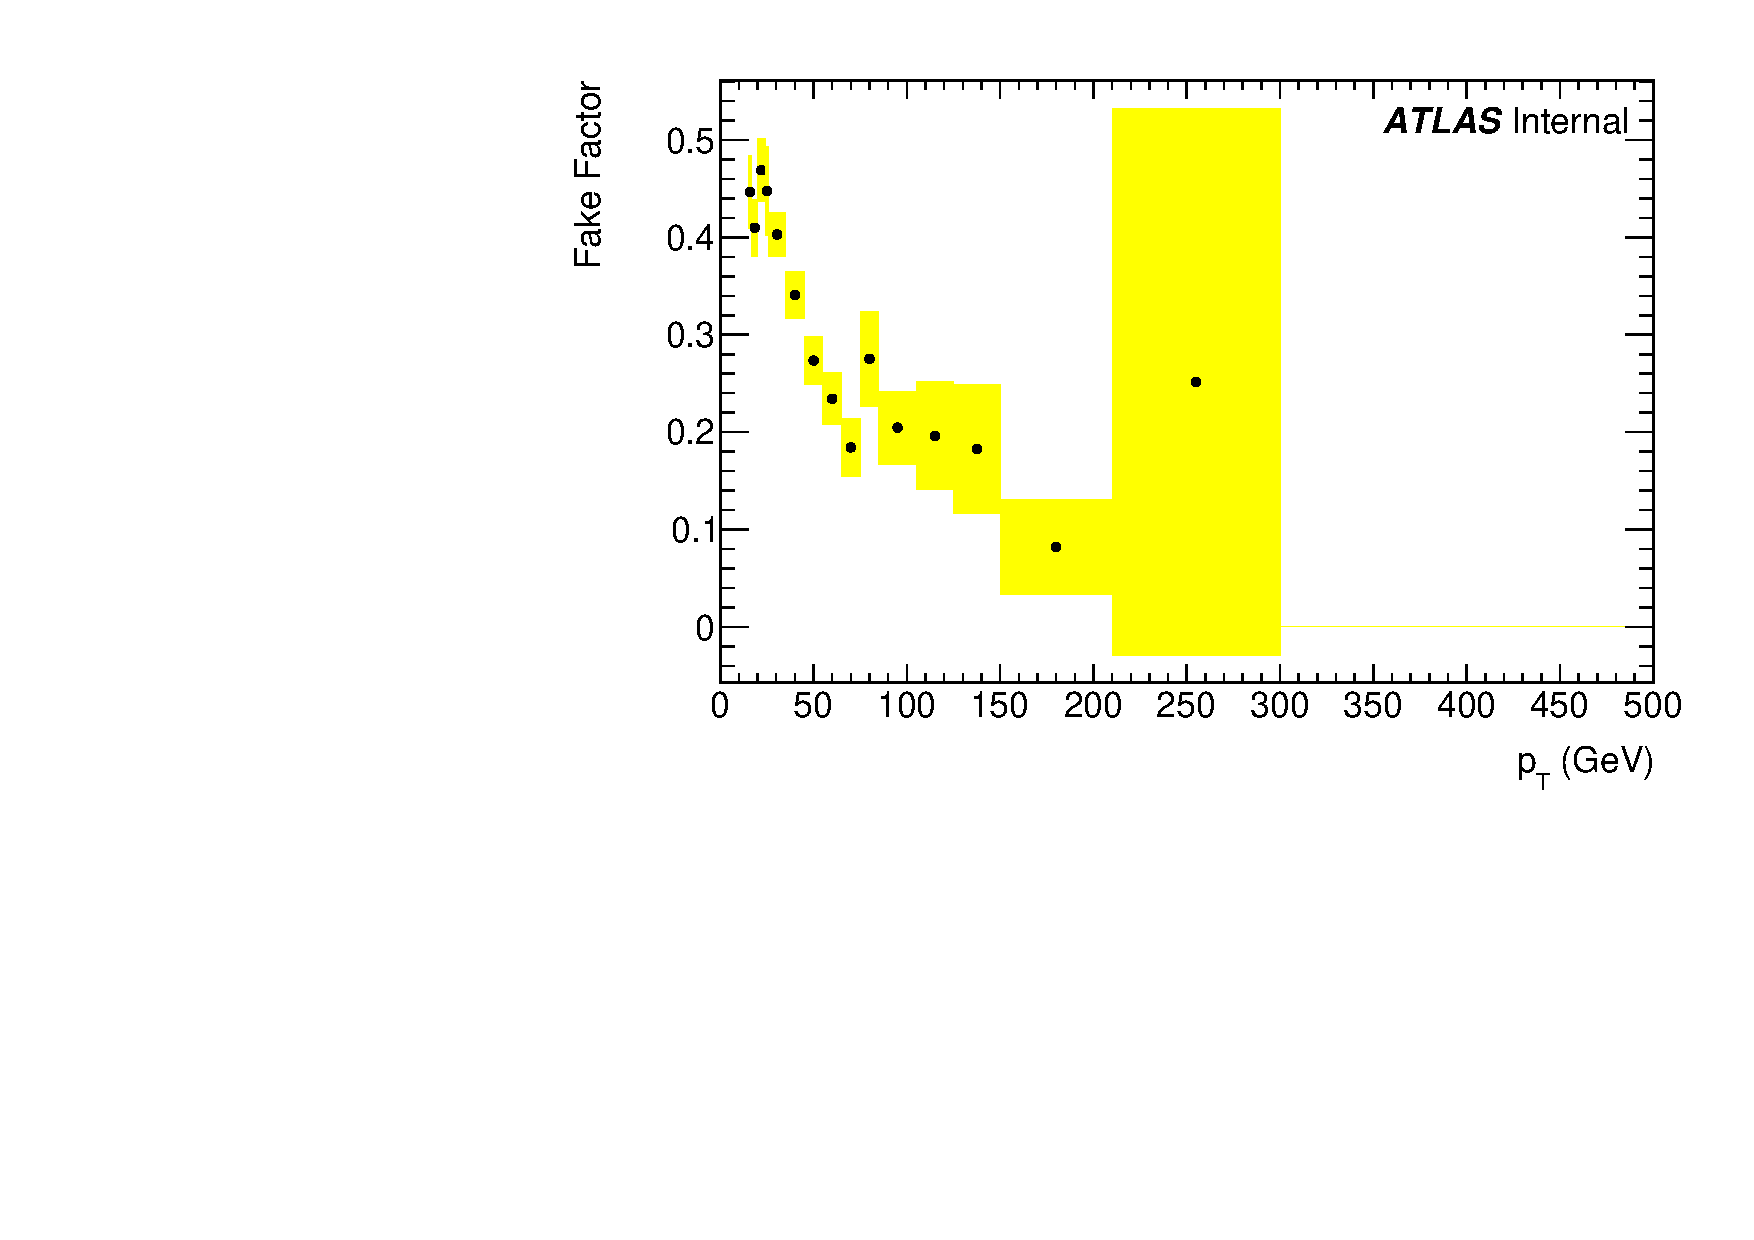
\includegraphics{figures/backgrounds/c_ff_lf_pt.pdf}}
    }
    \subfloat[Heavy Flavor] {
      \resizebox{3in}{!}{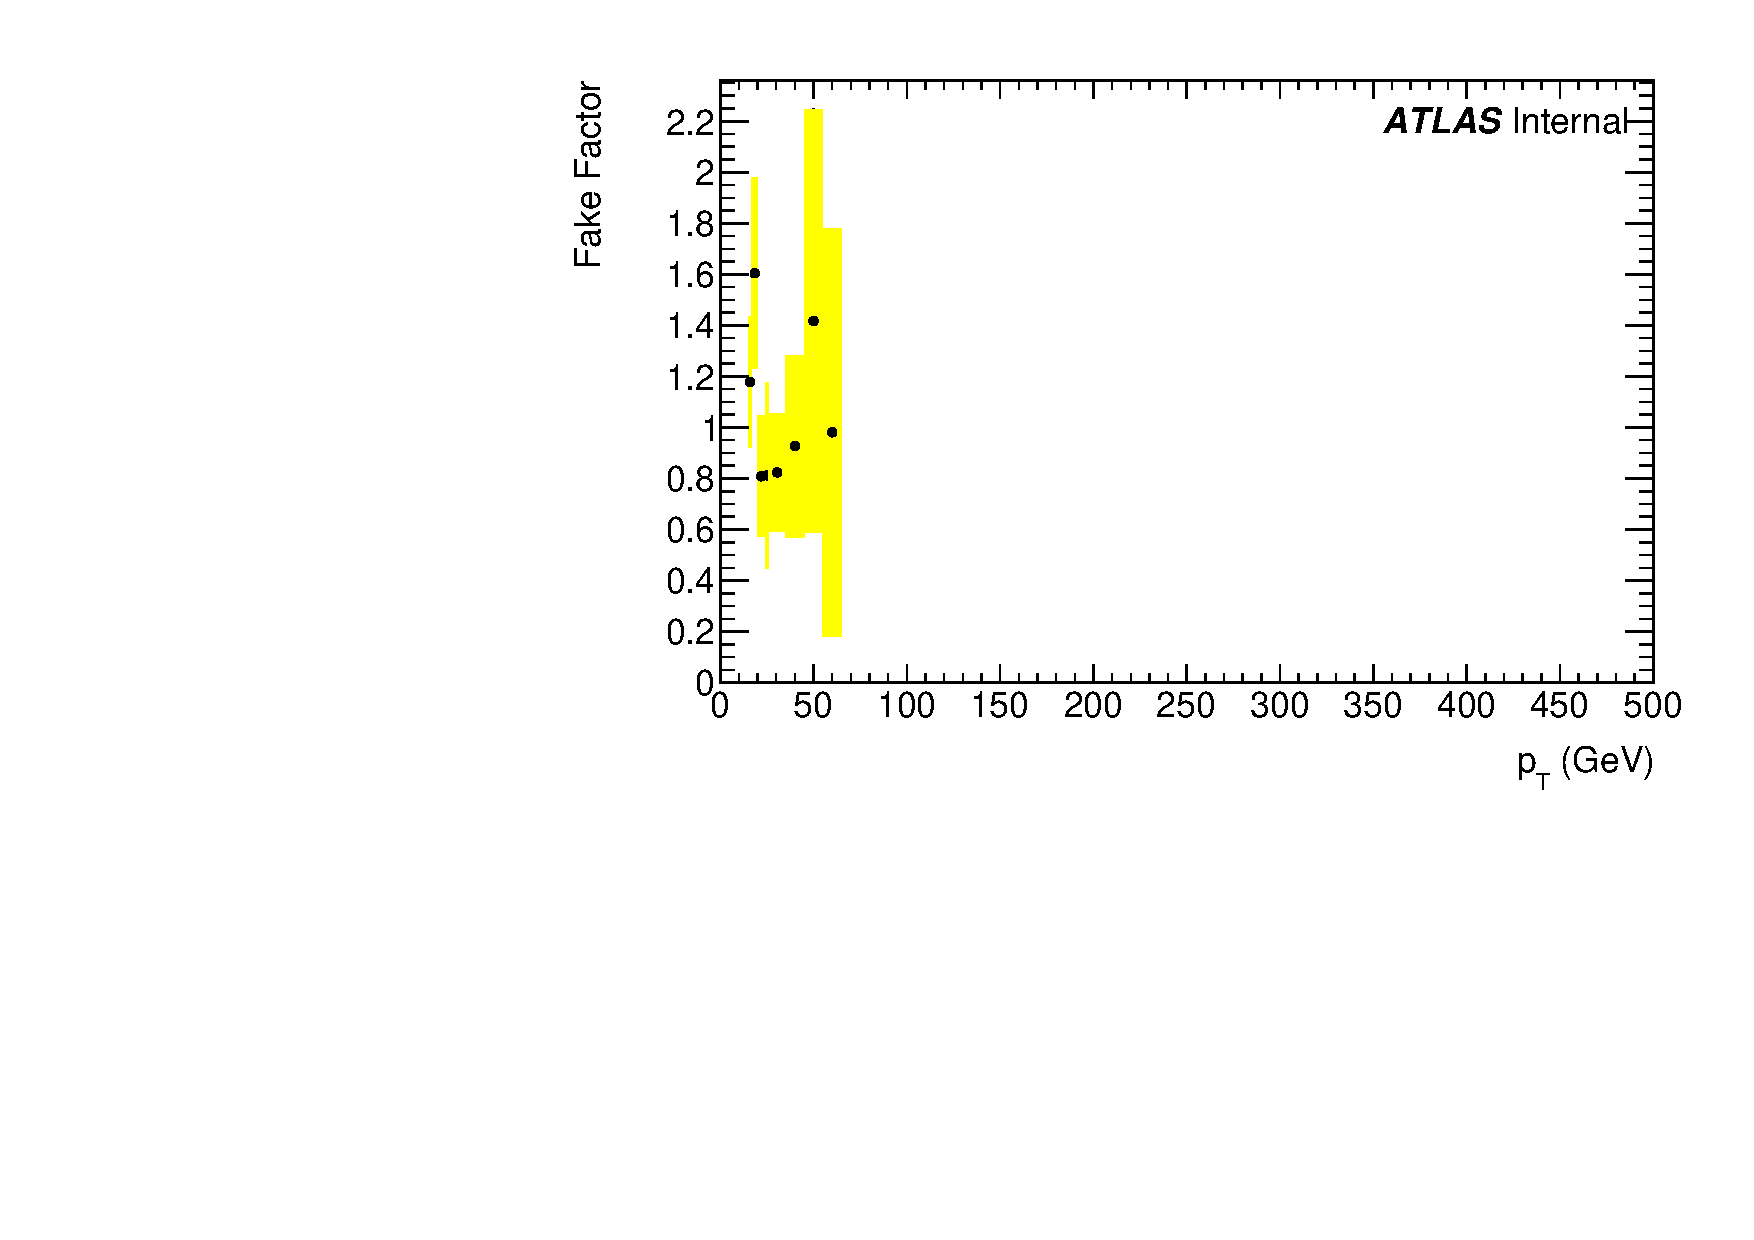
\includegraphics{figures/backgrounds/c_ff_hf_pt.pdf}}
    }
    \caption{MC fake factors for fakes from heavy and light flavor jets, from \mcatnlo\  $t\overline{t}$ Monte Carlo.}
    \label{fig:el-ff-ttbar}
  \end{figure}
  

  The fake factors in the control and signal regions can be expressed in terms of the truth heavy/light fake factors, $f_{H,L}$, and the fraction of denominators from heavy flavor, $\rho^{HF}$, by separating the numerators into heavy and light flavor truth origin:
  \begin{align}
      f_c &= \frac{N_N^{HF} + N_N^{LF}}{N_D}\\
          &= \frac{f_H \rho_c^{HF} N_D + f_L (1-\rho_c^{HF}) N_D}{N_D} = f_H \rho_c^{HF} + f_L (1-\rho_c^{HF})\\
      f_s &= \frac{f_H \rho_s^{HF} N_D + f_L (1-\rho_s^{HF}) N_D}{N_D} = f_H \rho_s^{HF} + f_L (1-\rho_s^{HF}).
  \end{align}

  The bias in fake factor is then given by the difference,

  \begin{align}\label{eq:hflf-bias}
    f_c - f_s &= (f_H - f_L) \times (\rho_c^{HF} - \rho_s^{HF})
  \end{align}

  The heavy flavor fraction in the denominator region are extracted using the truth $d_0$ significance distributions of heavy and light flavor fakes. In particular, in the MC sample, let $\rho_{HF}^{\textrm{high}}$ be the fraction of truth heavy flavor denominator objects that satisfy $\frac{d_0}{\sigma_{d_0}} > 3$, and similarly for light flavor. Then, in the data samples, the number of denominator objects with high $d_0$ significance is:
    \begin{align}
      N_{D, c}^{\textrm{high}} &= N_{D,c} \left( \rho_{c}^{HF} \rho_{HF}^{\textrm{high}} +  \rho_{c}^{LF} \rho_{LF}^{\textrm{high}} \right)\\ 
      \rho_{D,c}^{\textrm{high}}&= \left( \rho_{c}^{HF} \rho_{HF}^{\textrm{high}} +  (1-\rho_{c}^{HF}) \rho_{LF}^{\textrm{high}} \right)
    \end{align}
    Solving for $\rho_c^{HF}$,
    \begin{align}
      \rho_c^{HF} &= \frac{\rho_{D,c}^{\textrm{high}} - \rho_{LF}^{\textrm{high}}}{\rho_{HF}^{\textrm{high}} - \rho_{LF}^{\textrm{high}}}
    \end{align}
    The truth high-$d_0$ significance fractions for truth heavy and light flavor denominator objects are taken from the $t\overline{t}$ MC to be $\rho_{LF}^{\textrm{high}}=0.696$ and $\rho_{HF}^{\textrm{high}}=0.015$. 

  With these quantities, equation~\ref{eq:hflf-bias} gives the shift in fake factor value between the control and signal regions. The heavy flavor fractions extracted from the control and some signal regions are shown in table~\ref{t:el-ff-heavy-flavor-fractions}. Figure~\ref{fig:el-ff-syst-hflf} shows the percent variation in fake factor for a number of signal regions as a function of transverse momentum. The maximum deviation of $20\%$ is taken as a flat systematic uncertainty on the fake factors. 

  \begin{table}
    \centering
    \begin{tabular}{cc}
      Region & Heavy Flavor Fraction \\
      \hline
      Control        &  $ 0.031 \pm  0.006$ \\
      onZ / $e\mu$ / All      &  $-0.001 \pm  0.001$ \\
      onZ / $e\mu$ / Weak     &  $-0.003 \pm  0.001$ \\
      onZ / $e\mu$ / Strong   &  $ 0.021 \pm  0.007$ \\
      onZ / $e\mu$ / High MET  &  $-0.008 \pm  0.011$ \\
      onZ / $e\mu$ / Low MET   &  $-0.001 \pm  0.001$ \\
      offZ / $e\mu$ / All     &  $-0.004 \pm  0.003$ \\
      offZ / $e\mu$ / Weak    &  $-0.019 \pm  0.025$ \\
      offZ / $e\mu$ / Strong  &  $ 0.039 \pm  0.019$ \\
      offZ / $e\mu$ / High MET &  $ 0.003 \pm  0.003$ \\
      offZ / $e\mu$ / Low MET  &  $-0.006 \pm  0.003$ \\
      offZ / $e\mu$ / High $\mtw$ &  $ 0.026 \pm  0.020$ \\
    \end{tabular}
    \caption{Denominator object heavy flavor fractions in the control and signal regions, extracted using the fraction of events with $3<\frac{d_0}{\sigma_{d_0}}<10$.}
    \label{t:el-ff-heavy-flavor-fractions}
  \end{table}


  \begin{figure}
    \centering
    \resizebox{4in}{!}{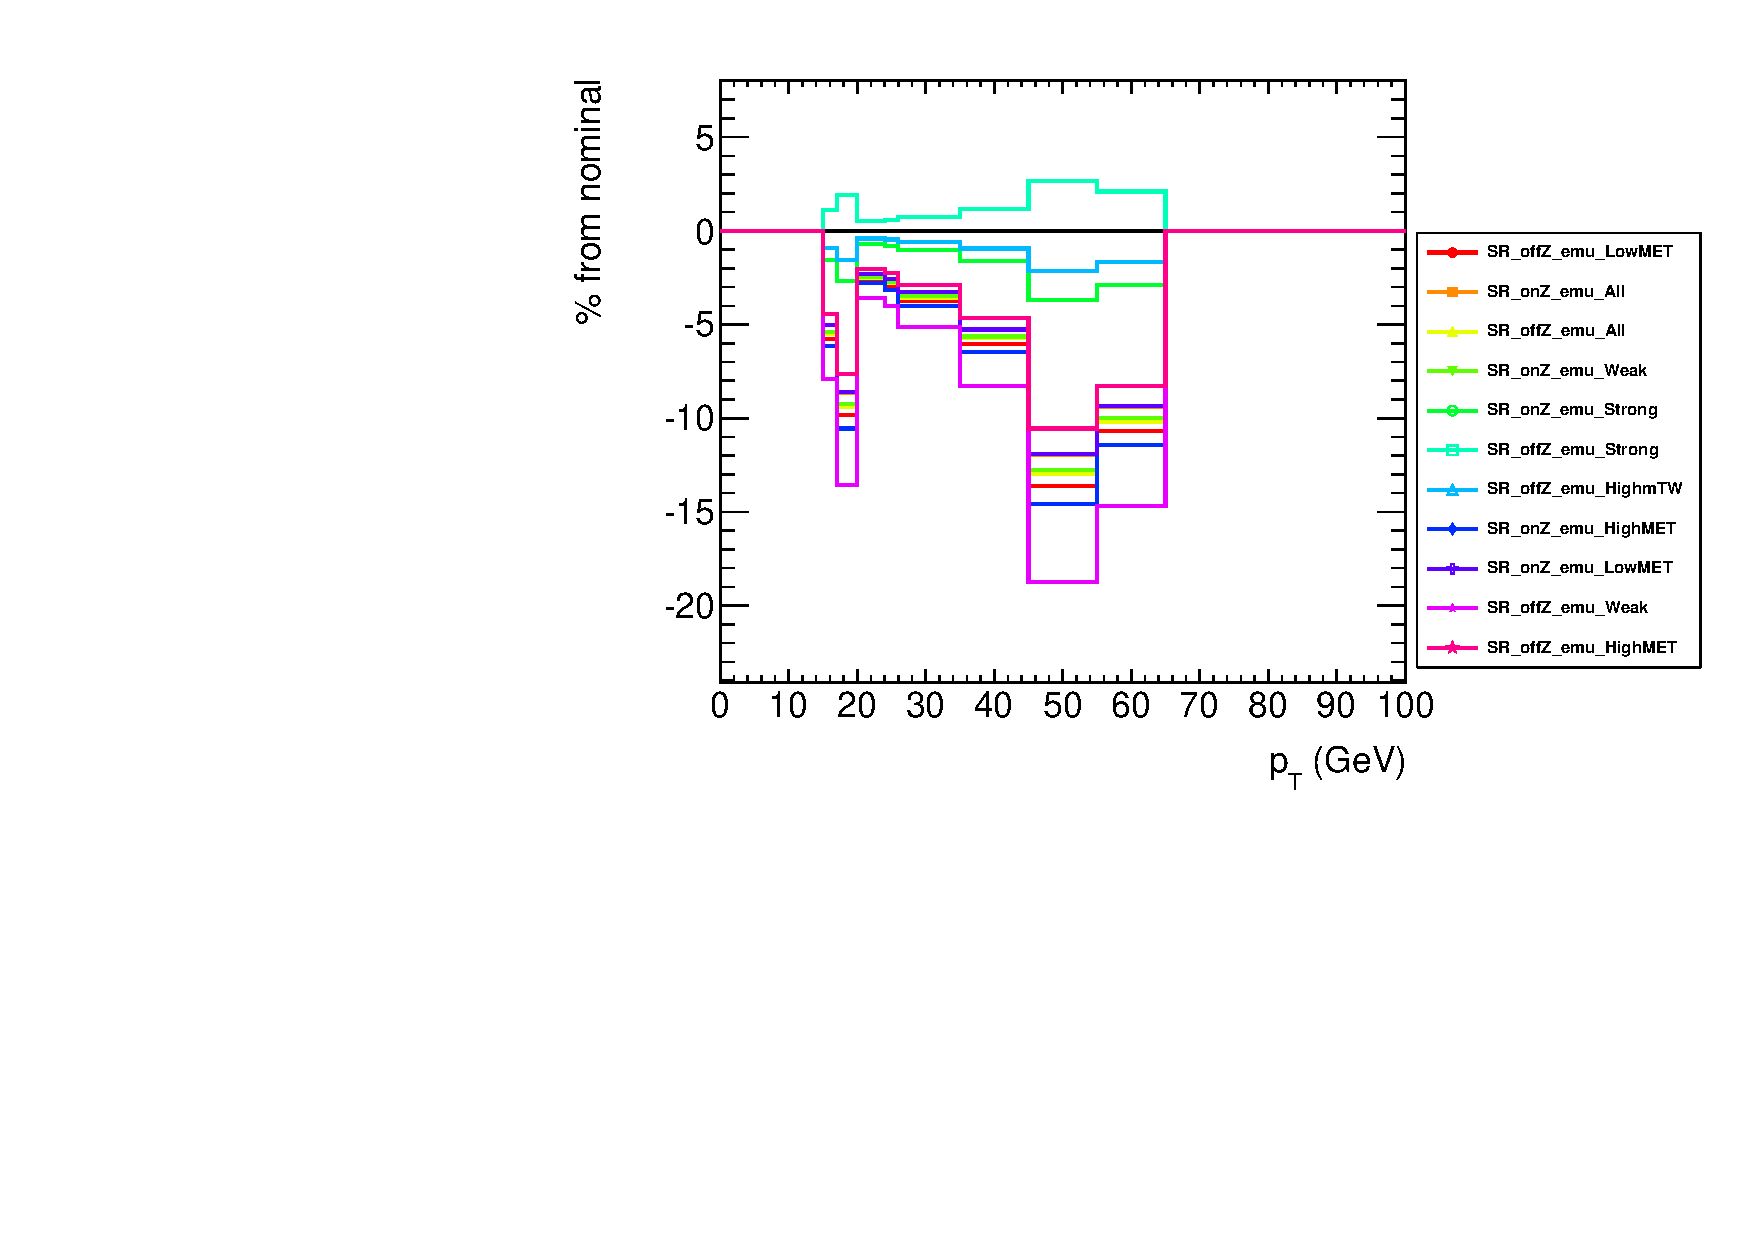
\includegraphics{figures/backgrounds/c_HFLF_systematic.pdf}}
    \caption{Percent deviation in fake factor between the control and signal regions due to variable heavy flavor fractions.}
    \label{fig:el-ff-syst-hflf}
  \end{figure}





\section{Trilepton Resonance Search}\label{sec:appendix-resonance}

\subsection{$\Delta R(Z,\ \ell_3)$ Cut Optimization}\label{sec:appendix-resonance-dr-optimization}

The value of the cut on the separation between the $Z$ candidate and the third lepton, $\Delta R(Z,\ \ell_3)$, is chosen based on a study of the expected sensitivity of the analysis at different values of the cut. The expected sensitivity is determined using a simple cut-and-count framework using narrow mass windows, rather than the fit-based framework. The half-width of the mass windows is taken from a linear fit to the full-width half-maxima of the signal peaks as determined from the signal fits (section~\ref{sec:appendix-resonance-signal-fits}). The expected 95\% CL exclusion on the signal cross section is then determined from the number of signal and background events inside the mass window predicted from Monte Carlo simulation, using the $\mathrm{CL}_s$ method (section~\ref{sec:appendix-cls}) implemented in the \texttt{mclimits} framework~\cite{Junk:2007wq}. 

The expected exclusions for cut values of $\Delta R < 2.0,\ 2.25,\ 2.5,\ 2.75,\ 3.0,\ 3.14,\ 3.5,$ and $4.0$ are shown in figure~\ref{fig:dR-optimization}. The same cut is applied to all signal categories, as no significant gain is observed by optimizing each cut individually. Smaller values of the cut ($\Delta R(Z,\ \ell_3)\lesssim 2.0$) perform similarly to more stringent cuts at low signal mass hypotheses, but perform worse at higher mass hypotheses. Cuts above $\Delta R(Z,\ \ell_3)\lesssim 3.0$ perform approximately equally. For simplicity, a flat cut value $\Delta R(Z,\ \ell_3)<3.0$ is chosen, independent of the mass hypothesis.


  \begin{figure}[h]
    \subfloat[Vector-Like Leptons] {
      \resizebox{0.45\textwidth}{!}{\includegraphics{figures/resonance/{c_limits_dRVariation_VLL_Combined_BRe1.0_BRmu0.0}.pdf}}
    }
    \subfloat[Type III Seesaw] {
      \resizebox{0.45\textwidth}{!}{\includegraphics{figures/resonance/{c_limits_dRVariation_Seesaw_Combined_BRe1.0_BRmu0.0}.pdf}}
    }
    \caption{Expected upper limits on the heavy lepton production cross section times branching ratio to final states with least one $Z(\ell\ell)+\ell$ decay for different cuts on the maximum value of $\Delta R(Z,\ \ell_3)$.}
    \label{fig:dR-optimization}
  \end{figure}


\subsection{Signal Fit Details}\label{sec:appendix-resonance-signal-fits}
Tables \ref{table:ZeFitParamsSS}-\ref{table:ZmuFitParamsVLL} show the results of fitting the Voigtian plus Landau function to each signal point for the type~III seesaw and vector-like leptons models. The fits are performed in the inclusive category in $Z+e$ and $Z+\mu$ flavor channels.  


\begin{table}[h]
 \centering
\scriptsize
\caption{Fit parameters for the type~III seesaw model in the $Z+e$ flavor channel and inclusive category. $m_V$, $\Gamma_V$, and $\sigma_V$ represent the mean, Lorentzian width, and Gaussian width of the Voigt function, and $m_L$ and $\sigma_L$ represent the mean and width of the Landau function. Note that the absence of the intrinsic width of the $Z$ boson in the simulation leads to smaller values than expected for the width of the Voigtian peak for masses below $\sim250 \GeV$.}
 \begin{tabular}{|c||c|c|c|c|c|c|}  
 \hline\hline
Mass [GeV] & $m_V$ [GeV] &  $\Gamma_V$ [GeV] &  $\sigma_V$ [GeV] & $m_L$  [GeV] & $\sigma_L$ [GeV] & Ratio\\
\hline \hline
$100 $&$ 8.7222   \pm0.015 $&$ 0.131 \pm0.04 $&$ 0.32\pm0.03 $&$ 36.1\pm0.7 $&$ 10.9\pm0.355118 $&$ 0.34$ \\ 
$120 $&$ 28.5035 \pm0.024 $&$ 0.594\pm0.12 $&$ 0.72\pm0.06 $&$ 34.1\pm0.8 $&$ 10.2\pm0.391391 $&$ 0.59$ \\
$160 $&$ 68.3224 \pm0.037 $&$ 1.34\pm0.15 $&$ 1.13\pm0.08 $&$ 45.9\pm0.7 $&$ 15.3\pm0.392333 $&$ 0.57 $\\
$200 $&$ 108.294 \pm0.052 $&$ 1.86\pm0.20 $&$ 1.59\pm0.10 $&$ 59.1\pm1.1 $&$ 21.3\pm0.568737 $&$ 0.58 $\\
$250 $&$ 158.039 \pm0.090 $&$ 3.08\pm0.37 $&$ 1.48\pm0.26 $&$ 75.6\pm2.1 $&$ 27.6\pm1.10452 $&$ 0.59$ \\ 
$300 $&$ 207.856 \pm0.129 $&$ 2.96\pm0.45 $&$ 2.75\pm0.23 $&$ 92.3\pm2.6 $&$ 35.7\pm1.39974 $&$ 0.55 $\\ 
$350 $&$ 257.775\pm0.169 $&$ 4.52\pm0.63 $&$ 3.21\pm0.33 $&$ 106.8\pm3.4 $&$ 41.6\pm1.85383 $&$ 0.57$ \\ 
$400 $&$ 308.066\pm0.198 $&$ 6.84\pm0.77 $&$ 2.77\pm0.48 $&$ 129.7\pm4.2 $&$ 51.3\pm2.34715 $&$ 0.55 $\\ 
$450 $&$ 357.463\pm0.277 $&$ 7.37\pm1.05 $&$ 3.91\pm0.61 $&$ 142.1\pm5.3 $&$ 58.3\pm3.06396 $&$ 0.54$ \\ 
$500 $&$ 407.731\pm0.262 $&$ 5.39\pm1.02 $&$ 5.26\pm0.53 $&$ 179.9\pm6.1 $&$ 71.5\pm3.65063   $&$ 0.52 $ \\
\hline\hline
\end{tabular} 
   \label{table:ZeFitParamsSS}
\end{table}


\begin{table}[h]
 \centering
\scriptsize
\caption{Fit parameters for the type~III seesaw model in the $Z+\mu$ flavor channel and inclusive category. $m_V$, $\Gamma_V$, and $\sigma_V$ represent the mean, Lorentzian width, and Gaussian width of the Voigt function, and $m_L$ and $\sigma_L$ represent the mean and width of the Landau function. Note that the absence of the intrinsic width of the $Z$ boson in the simulation leads to smaller values than expected for the width of the Voigtian peak for masses below $\sim250 \GeV$.}
 \begin{tabular}{|c||c|c|c|c|c|c|}  
 \hline\hline
Mass [GeV] & $m_V$ [GeV] &  $\Gamma_V$ [GeV] &  $\sigma_V$ [GeV] & $m_L$  [GeV] & $\sigma_L$ [GeV] & Ratio\\
\hline \hline
$100$&$8.78\pm0.01 $&$ 0.1\pm0.0$&$ 0.176\pm0.01 $&$ 35.6\pm0.5 $&$ 10.6\pm0.3 $&$0.45 $\\ 
$120$&$28.71\pm0.01 $&$ 0.28\pm0.057 $&$ 0.62\pm0.02 $&$ 31.2\pm0.5 $&$ 8.7\pm0.2 $&$0.60 $\\ 
$160$&$68.56\pm0.03 $&$ 1.86\pm0.14$&$ 1.18\pm0.08 $&$ 44.7\pm0.6 $&$ 15.3\pm0.3 $&$0.60 $\\ 
$200$&$108.3\pm0.05 $&$ 3.10\pm0.25 $&$ 1.99\pm0.13 $&$ 56.6\pm0.9 $&$ 19.4\pm0.5 $&$0.61$\\ 
$250$&$158.1\pm0.1 $&$ 4.36\pm0.61 $&$ 3.64\pm0.31 $&$ 73.6\pm1.9 $&$ 27.0\pm1.0 $&$0.61 $\\ 
$300$&$207.7\pm0.1 $&$ 8.17\pm0.84 $&$ 3.87\pm0.46 $&$ 86.2\pm2.4 $&$ 32.3\pm1.3 $&$0.61$ \\ 
$350$&$258.3\pm0.2 $&$ 10.04\pm1.44 $&$ 6.15\pm0.75 $&$ 103.1\pm3.2 $&$ 40.2\pm1.7 $&$0.59 $\\ 
$400$&$307.2\pm0.3 $&$ 13.09\pm1.69 $&$ 6.39\pm0.98 $&$ 120.9\pm4.2 $&$ 50.2\pm2.3 $&$0.58$ \\ 
$450$&$357.4\pm0.5 $&$ 18.08\pm3.05 $&$ 8.86\pm1.64 $&$ 137.7\pm5.9 $&$ 57.9\pm3.4 $&$0.56$ \\ 
$500$&$407.6\pm0.5 $&$ 14.20\pm3.10 $&$ 12.2\pm1.44 $&$ 166.7\pm6.1 $&$ 67.9\pm3.6 $&$0.53 $\\ 
\hline\hline
\end{tabular} 
   \label{table:ZmuFitParamsSS}
\end{table}


\begin{table}[h]
 \centering
\scriptsize
\caption{Fit parameters for the VLL model in the $Z+e$ flavor channel and inclusive category. $m_V$, $\Gamma_V$, and $\sigma_V$ represent the mean, Lorentzian width, and Gaussian width of the Voigt function, and $m_L$ and $\sigma_L$ represent the mean and width of the Landau function.}
\begin{tabular}{|c||c|c|c|c|c|c|} 
\hline\hline
Mass [GeV] & $m_V$ [GeV] &  $\Gamma_V$ [GeV] &  $\sigma_V$ [GeV] & $m_L$  [GeV] & $\sigma_L$ [GeV] & Ratio\\
\hline \hline
$100$&$10.77\pm0.18 $&$ 0.1\pm0.1 $&$ 2.5\pm0.2 $&$ 34.3\pm1.5 $&$ 12.12\pm0.47$&$0.37$\\ 
$110$&$18.54\pm0.04 $&$ 1.9\pm0.2 $&$ 1.0\pm0.1 $&$ 34.1\pm1.8 $&$ 10.08\pm0.51$&$0.69$\\ 
$120$&$28.25\pm0.04 $&$ 2.7\pm0.4 $&$ 0.7\pm0.2 $&$ 35.8\pm3.0 $&$ 10.95\pm1.02$&$0.75$ \\ 
$130$&$38.18\pm0.04 $&$ 2.2\pm0.2 $&$ 1.2\pm0.1$&$ 31.0\pm0.6 $&$ 9.40\pm0.32$&$0.71$ \\ 
$140$&$48.07\pm0.04 $&$ 2.2\pm0.2 $&$ 1.5\pm0.1 $&$ 33.4\pm0.6 $&$ 10.29\pm0.28$&$0.69$ \\ 
$160$&$68.00\pm0.04 $&$ 3.0\pm0.2 $&$ 1.4\pm0.1 $&$ 37.0\pm0.7 $&$ 11.52\pm0.32$&$0.70$ \\ 
$180$&$87.97\pm0.05 $&$ 3.2\pm0.2 $&$ 1.6\pm0.1 $&$ 43.8\pm0.7 $&$ 14.05\pm0.35$&$0.67$ \\ 
$200$&$107.89\pm0.05 $&$ 3.0\pm0.2 $&$ 2.0\pm0.1 $&$ 49.7\pm0.8 $&$ 16.38\pm0.39$&$0.65$ \\ 
$250$&$157.75\pm0.06 $&$ 3.2\pm0.2 $&$ 2.6\pm0.2 $&$ 66.2\pm0.9 $&$ 22.76\pm0.47$&$0.59$ \\ 
$300$&$207.57\pm0.07 $&$ 3.4\pm0.3 $&$ 3.3\pm0.2 $&$ 83.9\pm1.1 $&$ 29.64\pm0.58$&$0.57$ \\ 
$400$&$307.53\pm0.09 $&$ 4.2\pm0.3 $&$ 4.4\pm0.2 $&$ 118.9\pm1.7 $&$ 46.42\pm0.93$&$0.53$ \\ 
 \hline\hline
\end{tabular} 
   \label{table:ZeFitParamsVLL}
\end{table}


\begin{table}[h]
 \centering
\scriptsize
\caption{Fit parameters for the VLL model in the $Z+\mu$ flavor channel and inclusive category. $m_V$, $\Gamma_V$, and $\sigma_V$ represent the mean, Lorentzian width, and Gaussian width of the Voigt function, and $m_L$ and $\sigma_L$ represent the mean and width of the Landau function.}
\begin{tabular}{|c||c|c|c|c|c|c|} 
 \hline\hline
Mass [GeV] & $m_V$ [GeV] &  $\Gamma_V$ [GeV] &  $\sigma_V$ [GeV] & $m_L$  [GeV] & $\sigma_L$ [GeV] & Ratio\\
\hline \hline
$100$&$10.9\pm0.13 $&$ 0.1\pm0.05 $&$ 2.85\pm0.10 $&$ 35.63\pm1.21 $&$ 11.98\pm0.40$&$0.44$\\
$110$&$18.7\pm0.03$&$ 2.13\pm0.16 $&$ 0.73\pm0.11 $&$ 32.88\pm1.55 $&$ 9.47\pm0.46$&$0.74$\\
$120$&$28.5\pm0.03 $&$ 2.26\pm0.19 $&$ 0.78\pm0.11 $&$ 30.72\pm1.17 $&$ 9.44\pm0.59$&$0.75$\\
$130$&$38.4\pm0.03 $&$ 2.23\pm0.16 $&$ 1.07\pm0.09 $&$ 29.40\pm0.48 $&$ 8.83\pm0.26$&$0.73$\\
$140$&$48.5\pm0.03$&$ 2.38\pm0.16 $&$ 1.26\pm0.09 $&$ 30.57\pm0.50 $&$ 9.31\pm0.25$&$0.73$\\
$160$&$68.5\pm0.05 $&$ 2.71\pm0.19 $&$ 1.74\pm0.10 $&$ 33.97\pm0.55 $&$ 10.45\pm0.27$&$0.71$\\
$180$&$88.3\pm0.05 $&$ 2.73\pm0.21 $&$ 2.19\pm0.11 $&$ 40.06\pm0.62 $&$ 12.76\pm0.30$&$0.68$\\
$200$&$108.4\pm0.1 $&$ 3.34\pm0.26 $&$ 2.81\pm0.14 $&$ 45.44\pm0.65 $&$ 14.28\pm0.32$&$0.66$\\
$250$&$158.2\pm0.1 $&$ 4.45\pm0.34 $&$ 3.89\pm0.17 $&$ 61.10\pm0.85 $&$ 20.71\pm0.42$&$0.62$\\
$300$&$208.0\pm0.1 $&$ 6.21\pm0.48 $&$ 5.26\pm0.25 $&$ 76.50\pm1.01 $&$ 26.62\pm0.51$&$0.58$\\
$400$&$307.9\pm0.2 $&$ 9.12\pm0.84 $&$ 8.63\pm0.40 $&$ 114.84\pm1.60 $&$ 42.99\pm0.85$&$0.53$\\
\hline\hline
\end{tabular} 
   \label{table:ZmuFitParamsVLL}
\end{table}



\subsection{Additional Kinematic Distributions}\label{sec:appendix-resonance-SR-distributions}
This section shows the $m_{3\ell}$, $\Delta R(Z,\ \ell_3)$, $\mtw$, and $\Etmiss$ distributions in each of the signal regions (the primary distributions are shown in section~\ref{sec:resonance-results}).

\begin{figure}[h]
  \centering
  \subfloat[ $Z+e$, inclusive] {
    \resizebox{0.48\textwidth}{!}{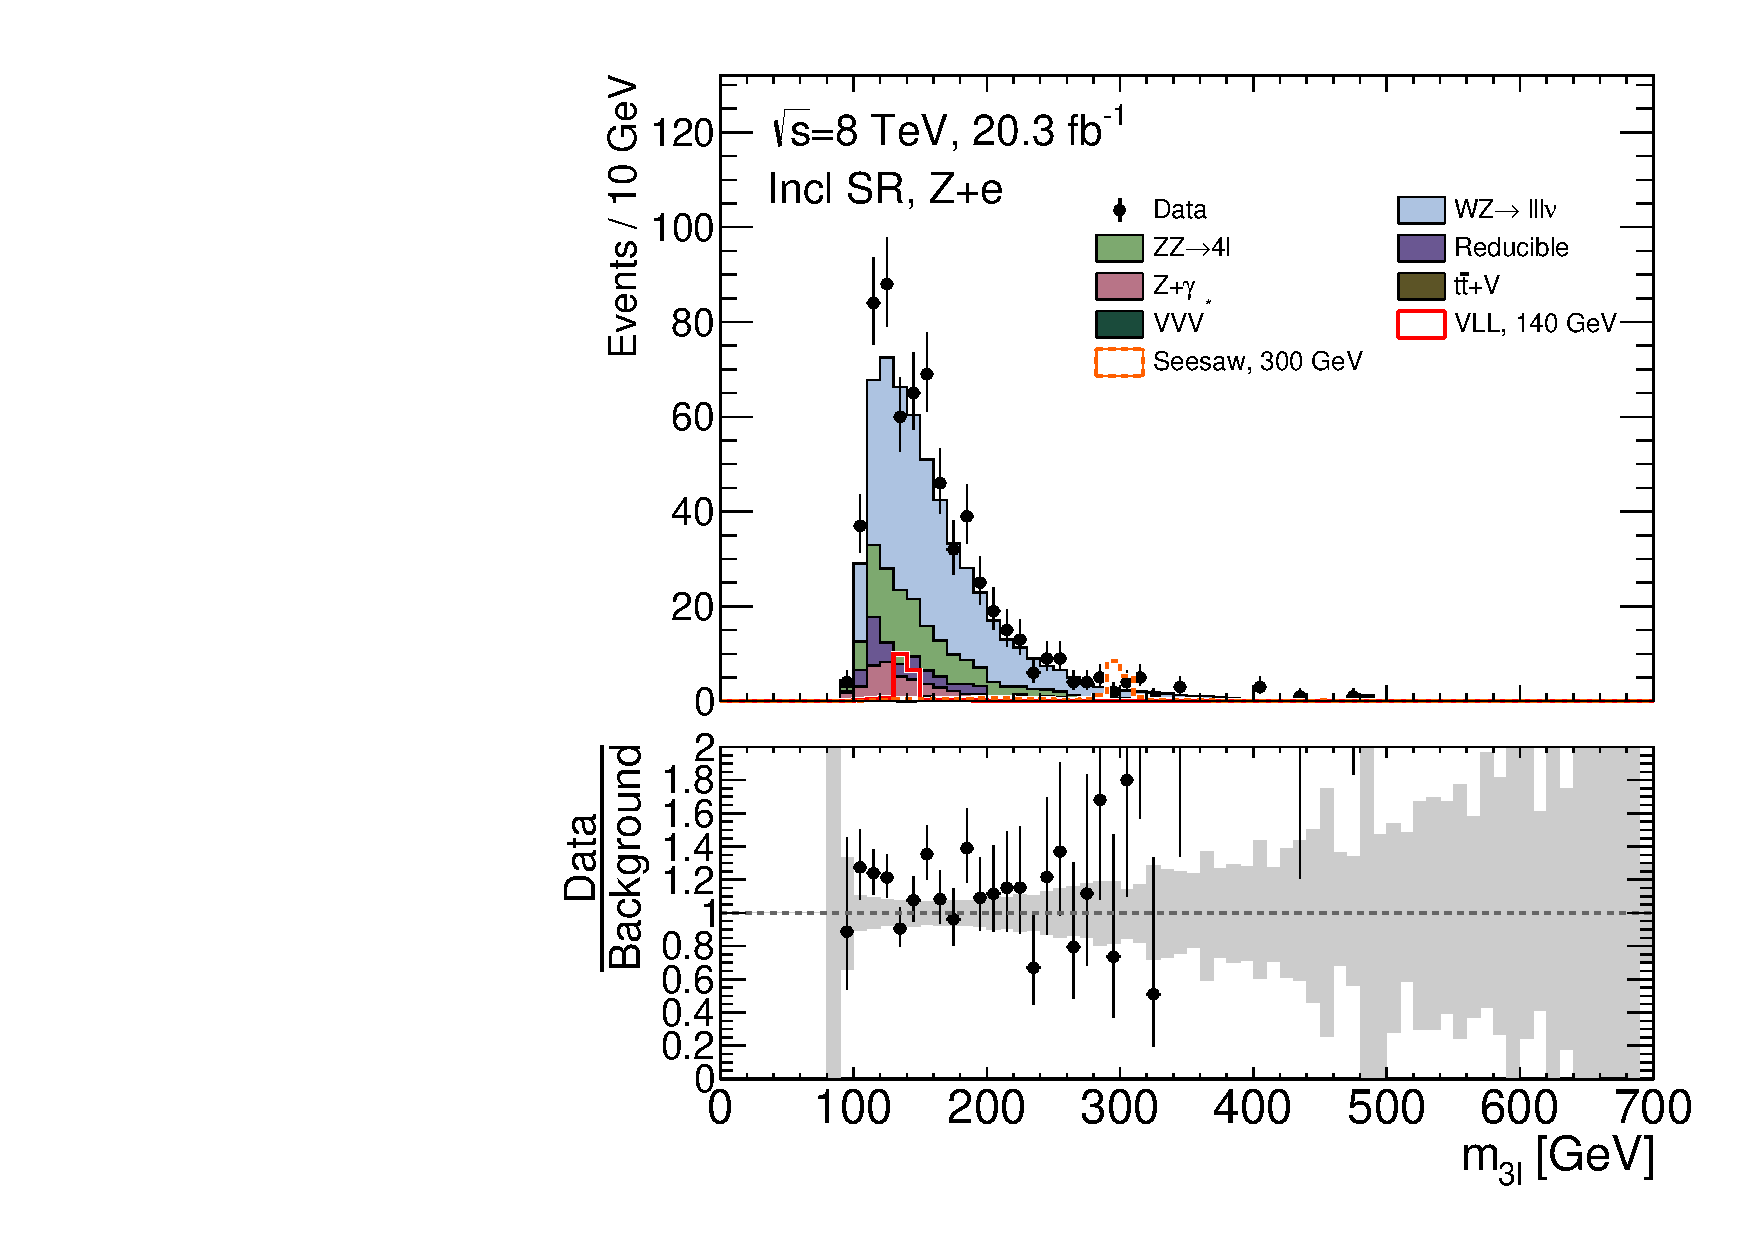
\includegraphics{figures/resonance/c_output_m3l_Ze_InclusiveNoM3L_300GeV}}
  }
  \subfloat[ $Z+\mu$, inclusive] {
    \resizebox{0.48\textwidth}{!}{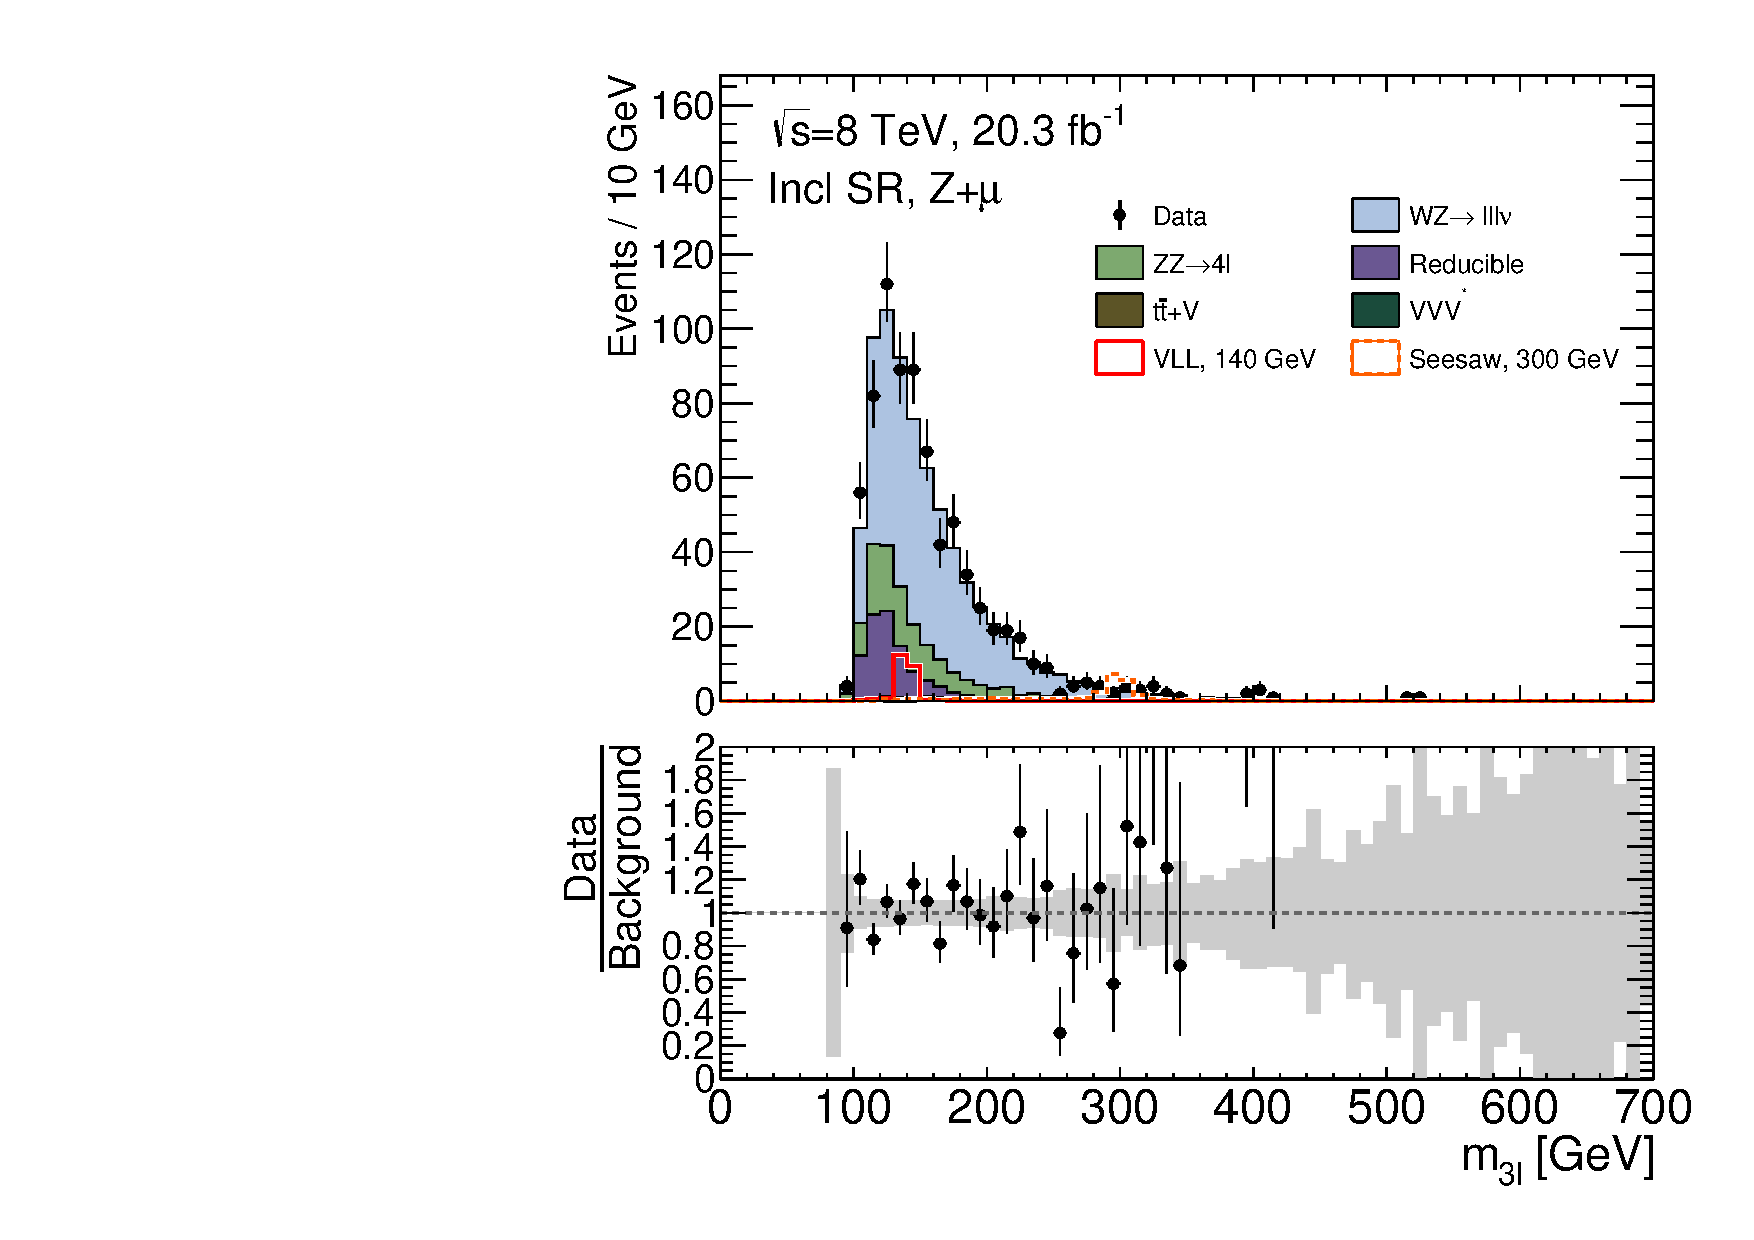
\includegraphics{figures/resonance/c_output_m3l_Zmu_InclusiveNoM3L_300GeV}}
  } \\
  \subfloat[ $Z+e$, $\fourl$ category] {
    \resizebox{0.48\textwidth}{!}{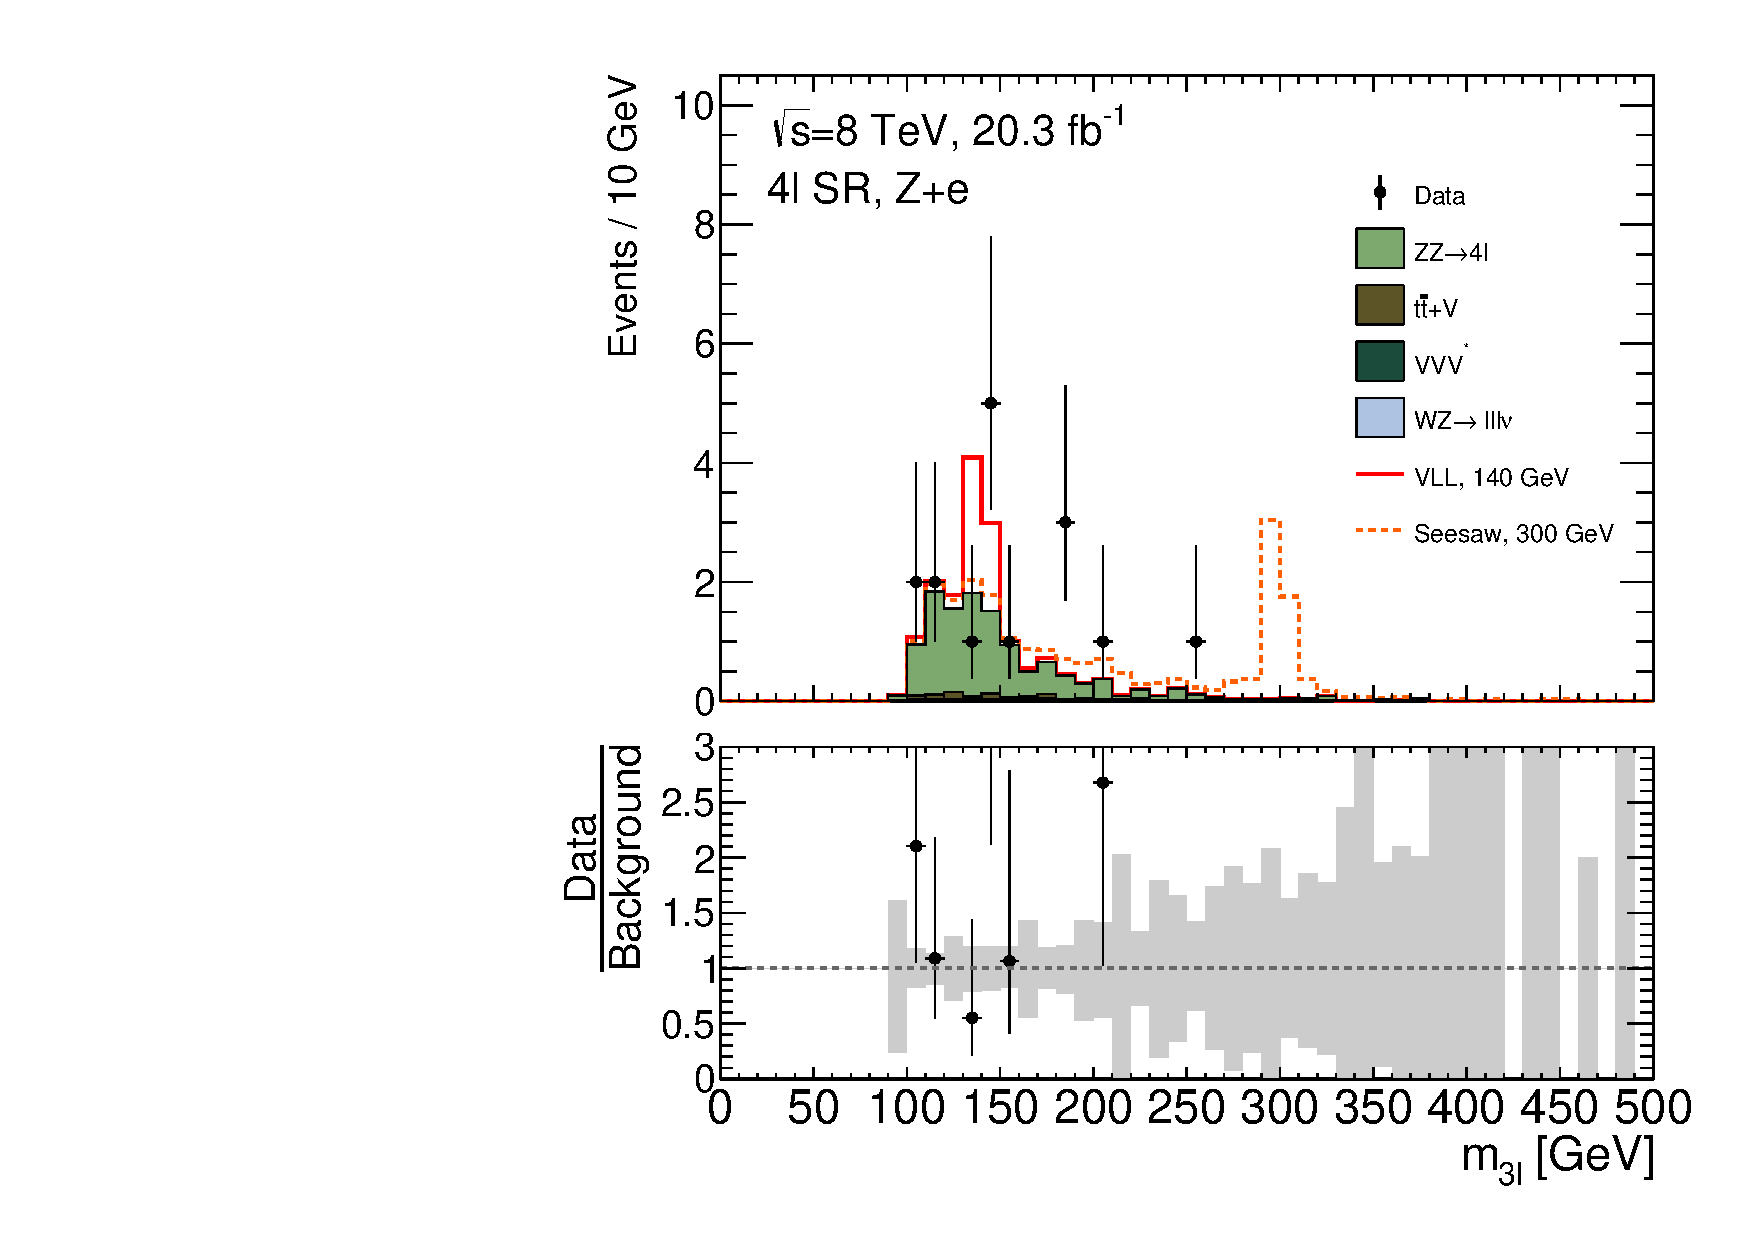
\includegraphics{figures/resonance/c_output_m3l_Ze_FourLNoM3L_300GeV}}
  }
  \subfloat[ $Z+\mu$, $\fourl$ category] {
    \resizebox{0.48\textwidth}{!}{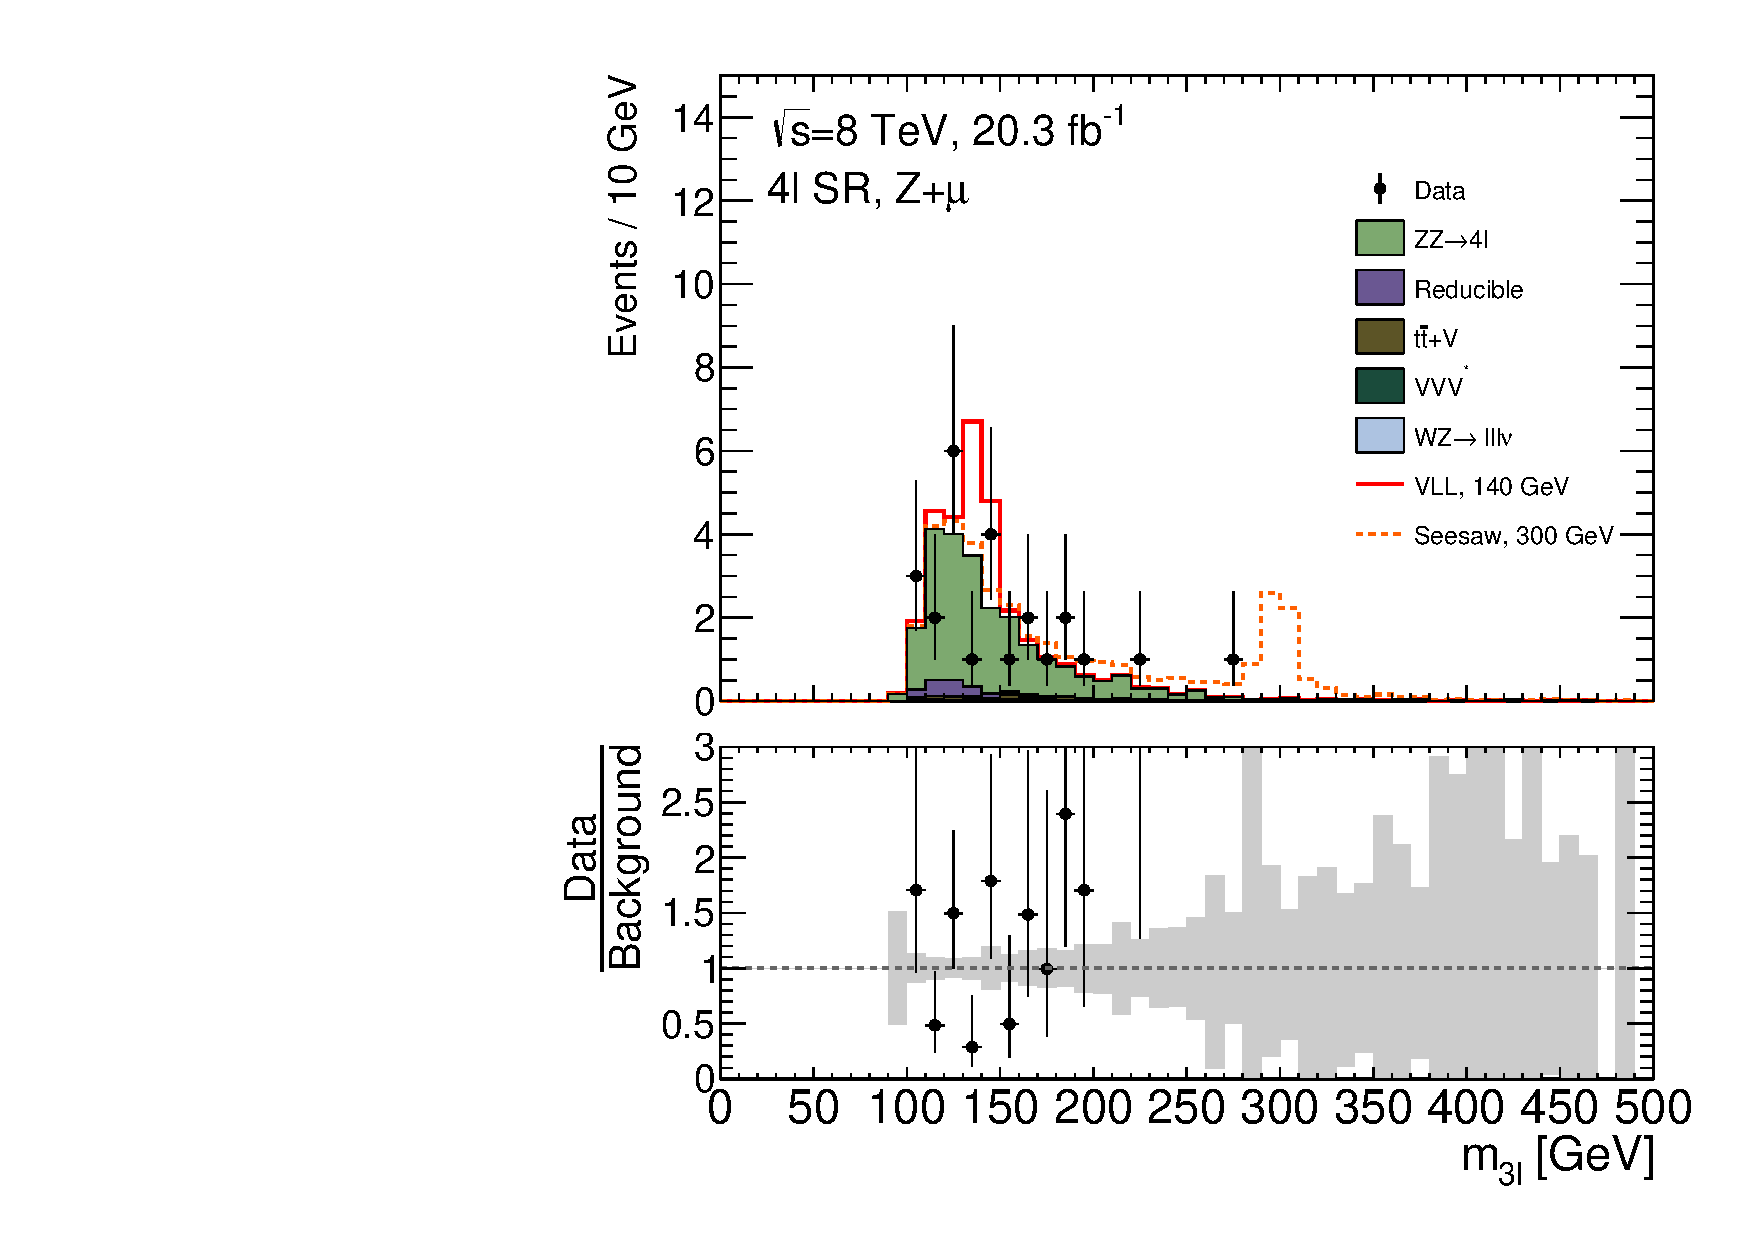
\includegraphics{figures/resonance/c_output_m3l_Zmu_FourLNoM3L_300GeV}}
  } \\
  \caption{$m_{3\ell}$ distributions for $Z+e$ and $Z+\mu$ candidates, for the inclusive and $\fourl$ signal regions (linear scale).}
  \label{fig:SR-m3l-1-linear}
\end{figure}

\begin{figure}[h]
  \centering
  \subfloat[ $Z+e$, dijet category] {
    \resizebox{0.48\textwidth}{!}{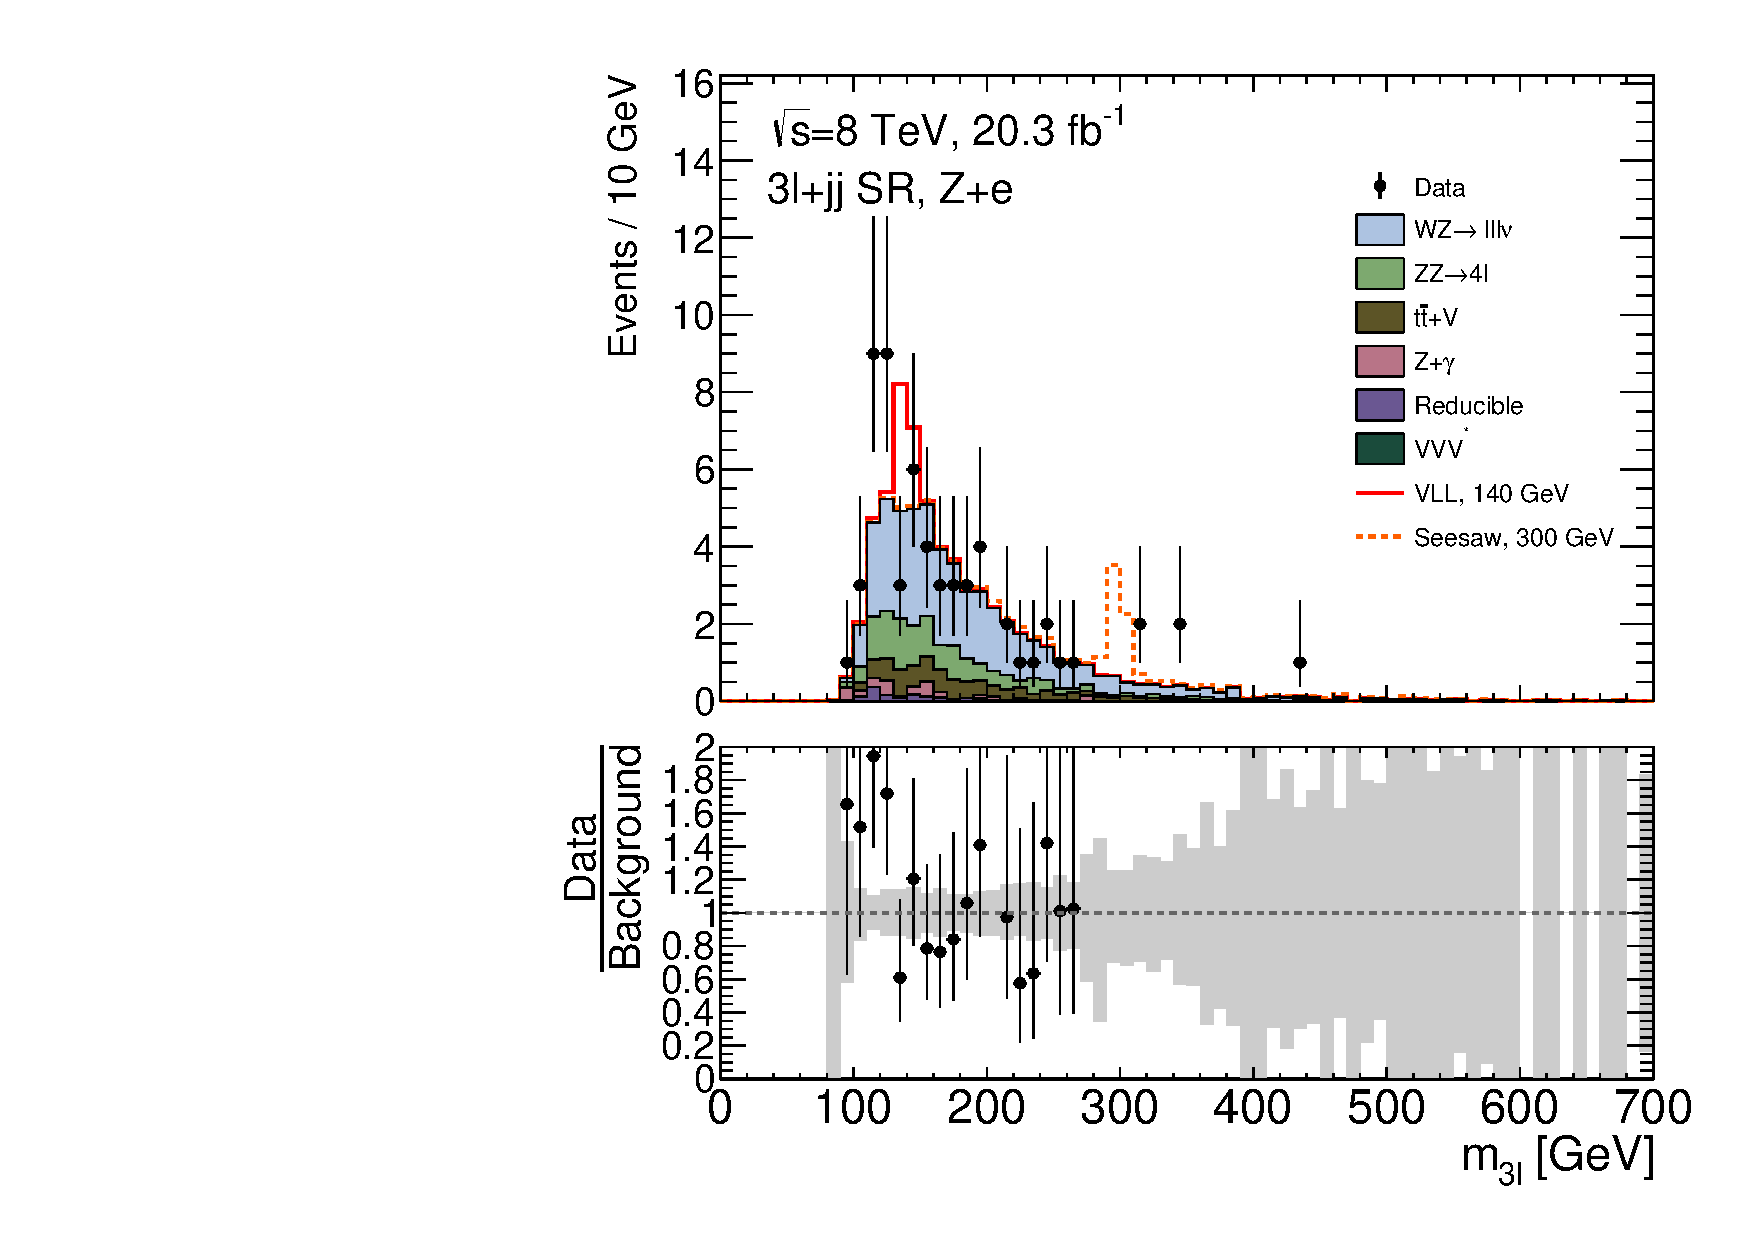
\includegraphics{figures/resonance/c_output_m3l_Ze_ThreeLDijetNoM3L_300GeV}}
  }
  \subfloat[ $Z+\mu$, dijet category] {
    \resizebox{0.48\textwidth}{!}{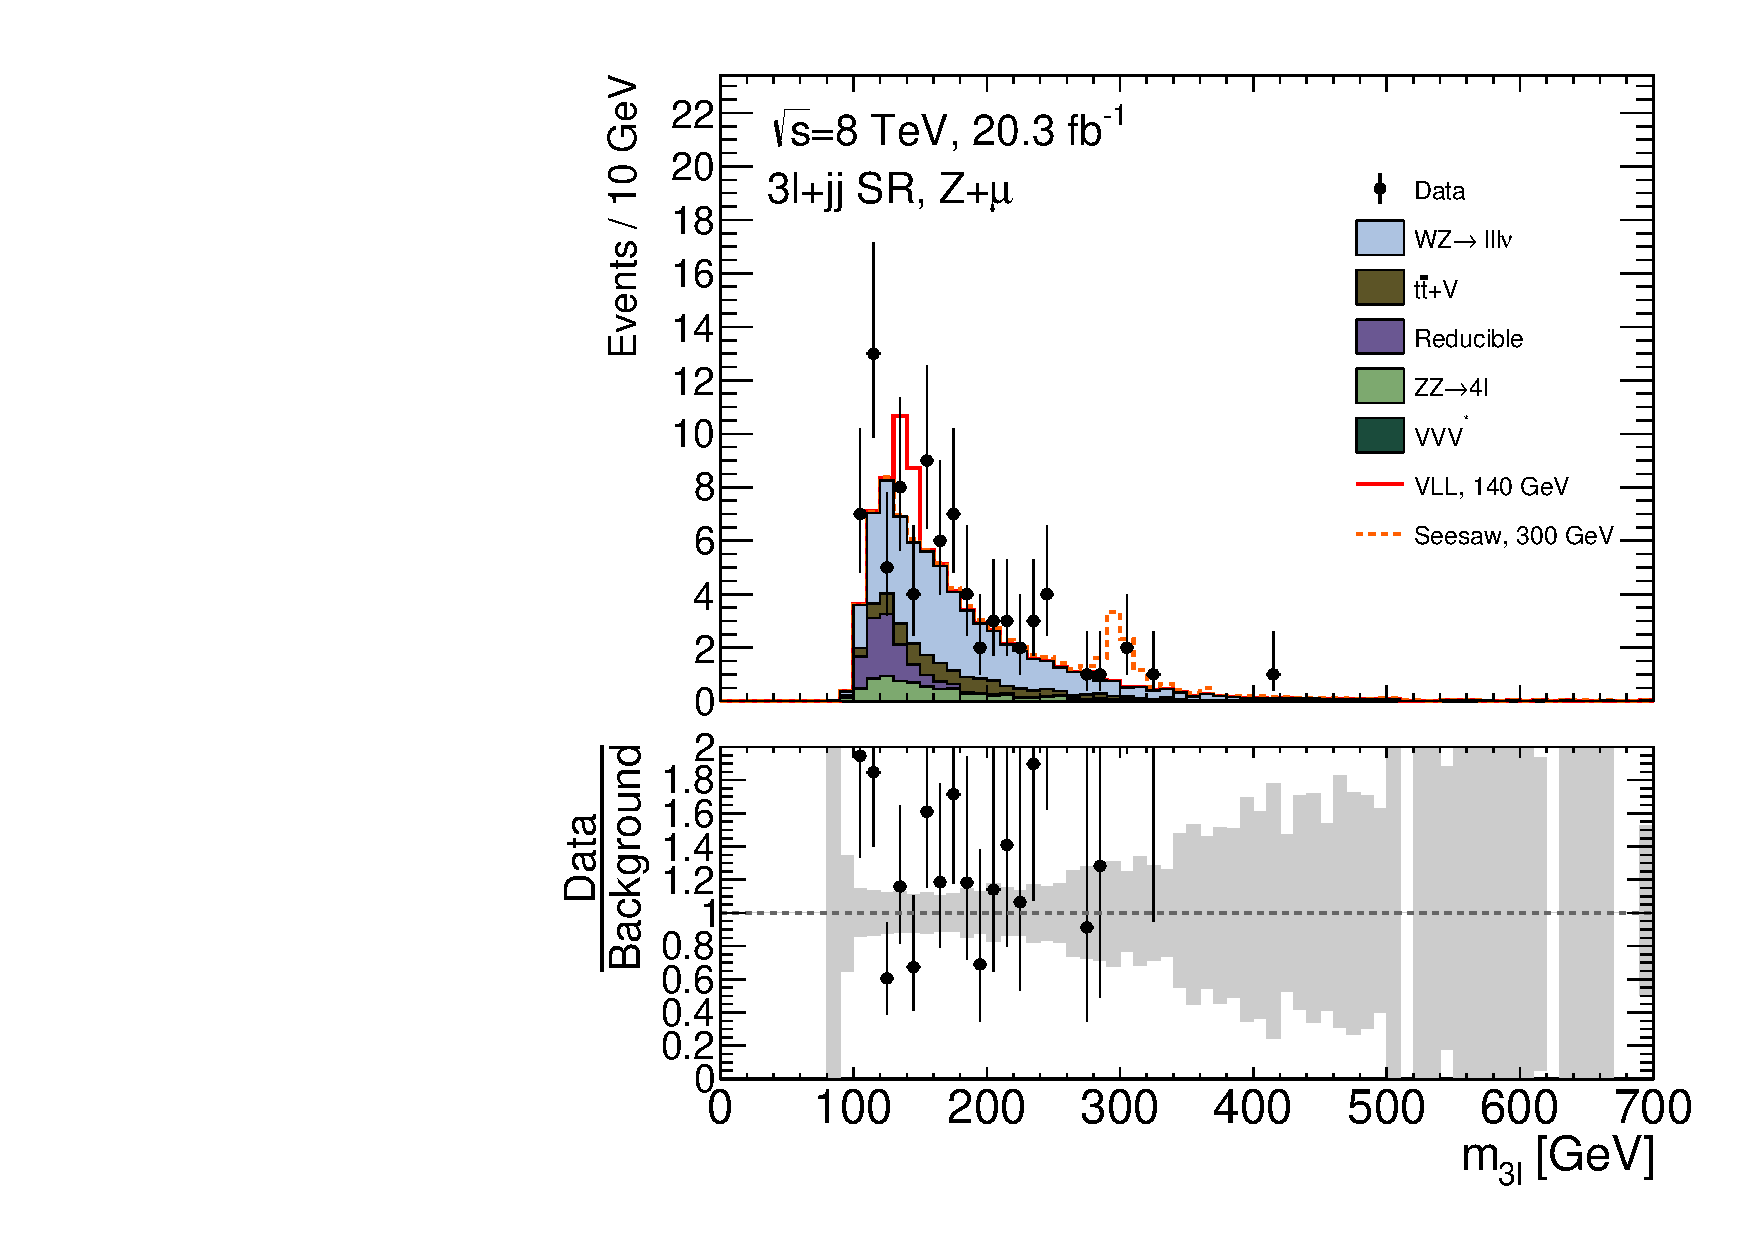
\includegraphics{figures/resonance/c_output_m3l_Zmu_ThreeLDijetNoM3L_300GeV}}
  } \\
  \subfloat[ $Z+e$, else category] {
    \resizebox{0.48\textwidth}{!}{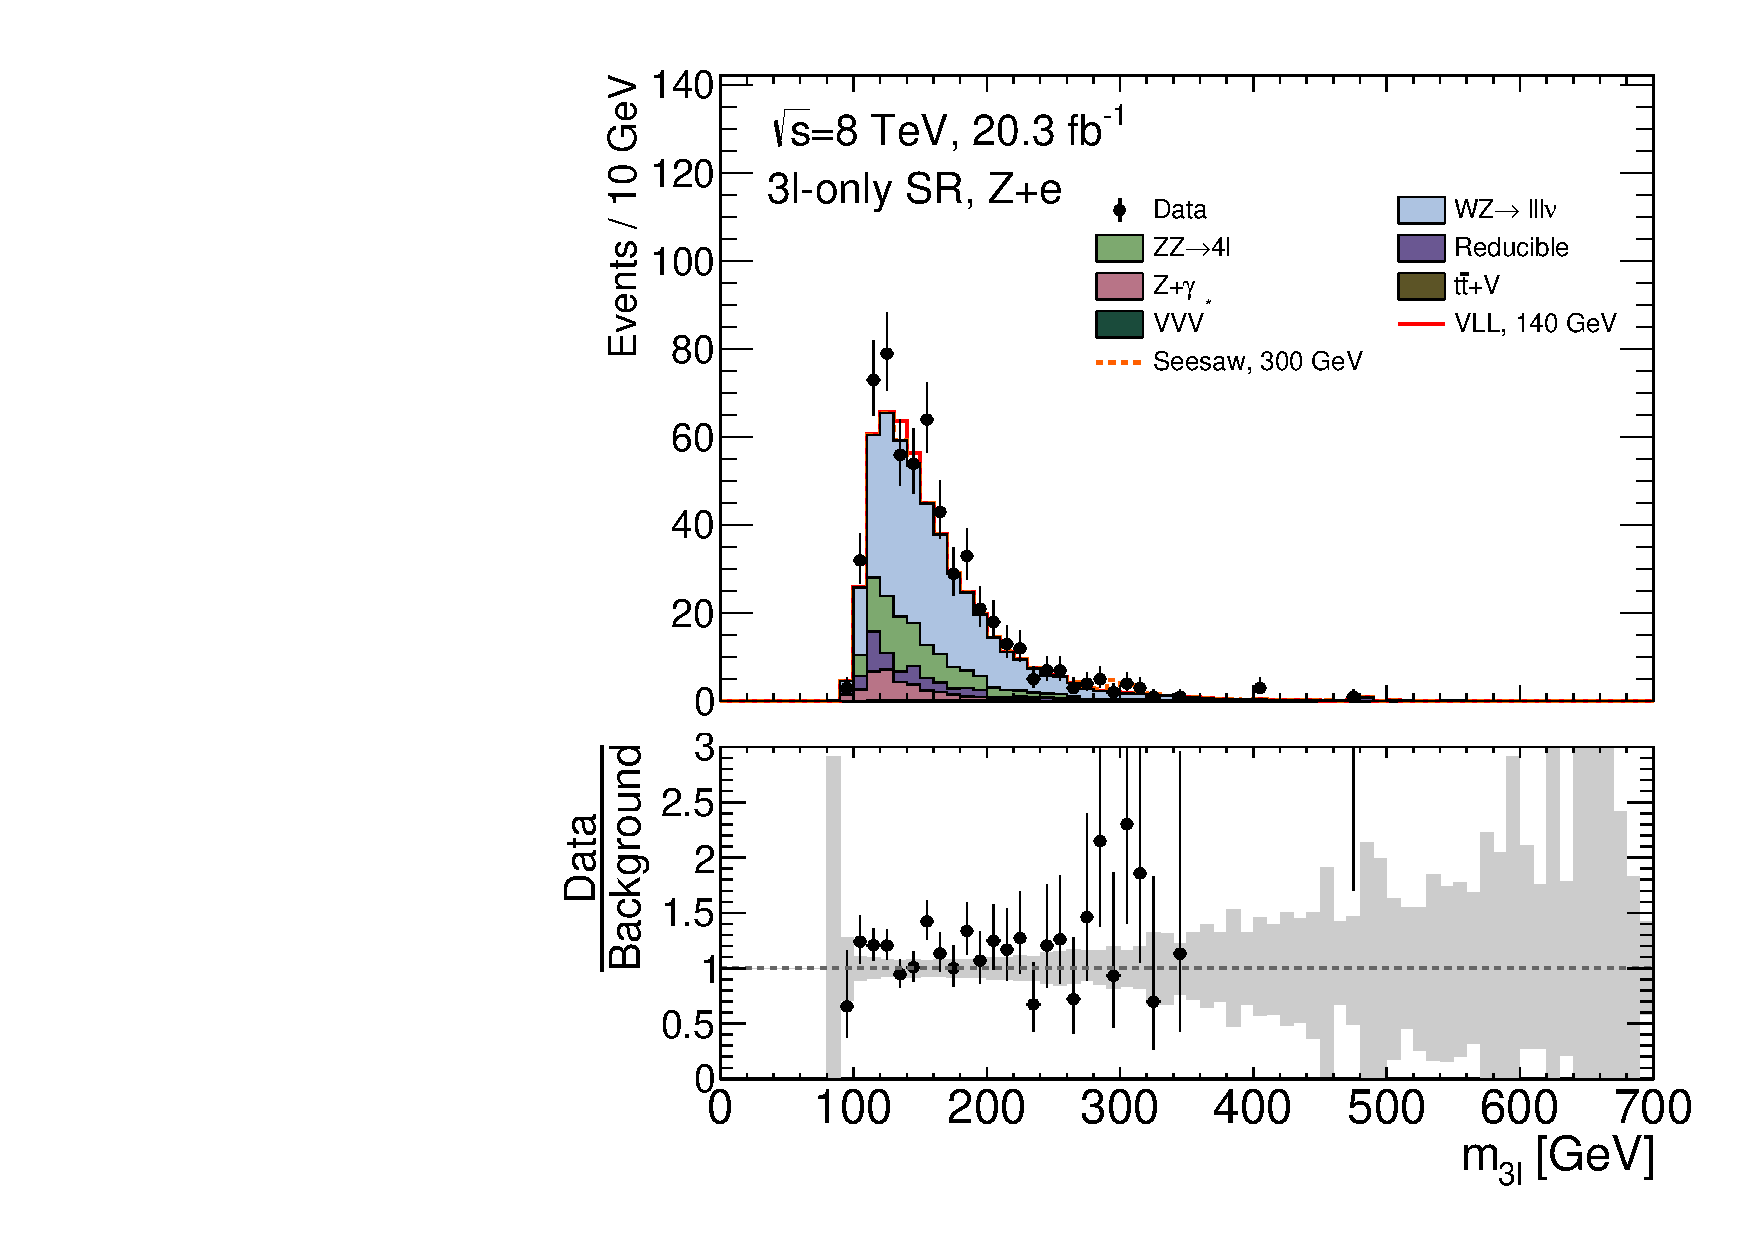
\includegraphics{figures/resonance/c_output_m3l_Ze_ElseNoM3L_300GeV}}
  }
  \subfloat[ $Z+\mu$, else category] {
    \resizebox{0.48\textwidth}{!}{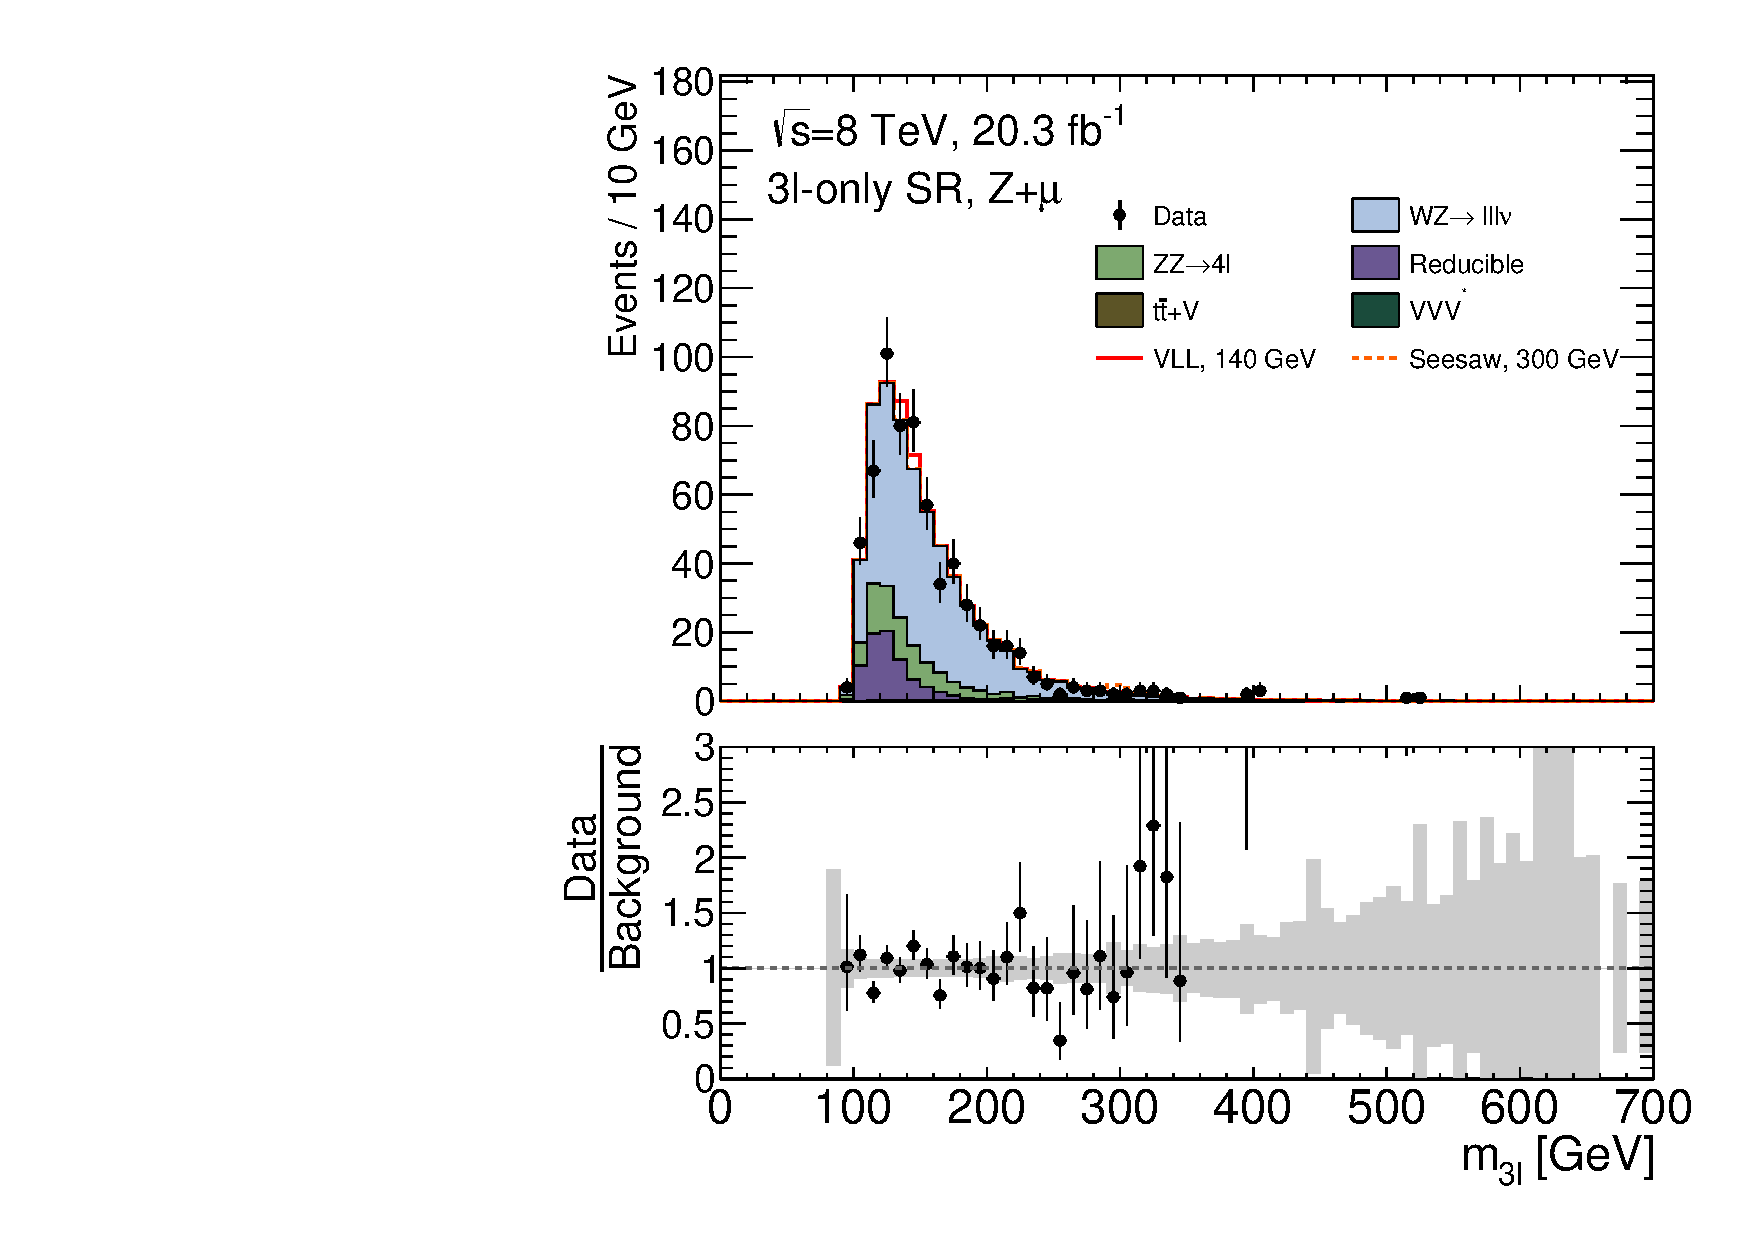
\includegraphics{figures/resonance/c_output_m3l_Zmu_ElseNoM3L_300GeV}}
  }
  \caption{$m_{3\ell}$ distributions for $Z+e$ and $Z+\mu$ candidates, for the $\threeljj$ and $\threelo$ signal regions (linear scale).}
  \label{fig:SR-m3l-2-linear}
\end{figure}


\begin{figure}[h]
  \centering
  \subfloat[ $Z+e$, inclusive] {
    \resizebox{0.48\textwidth}{!}{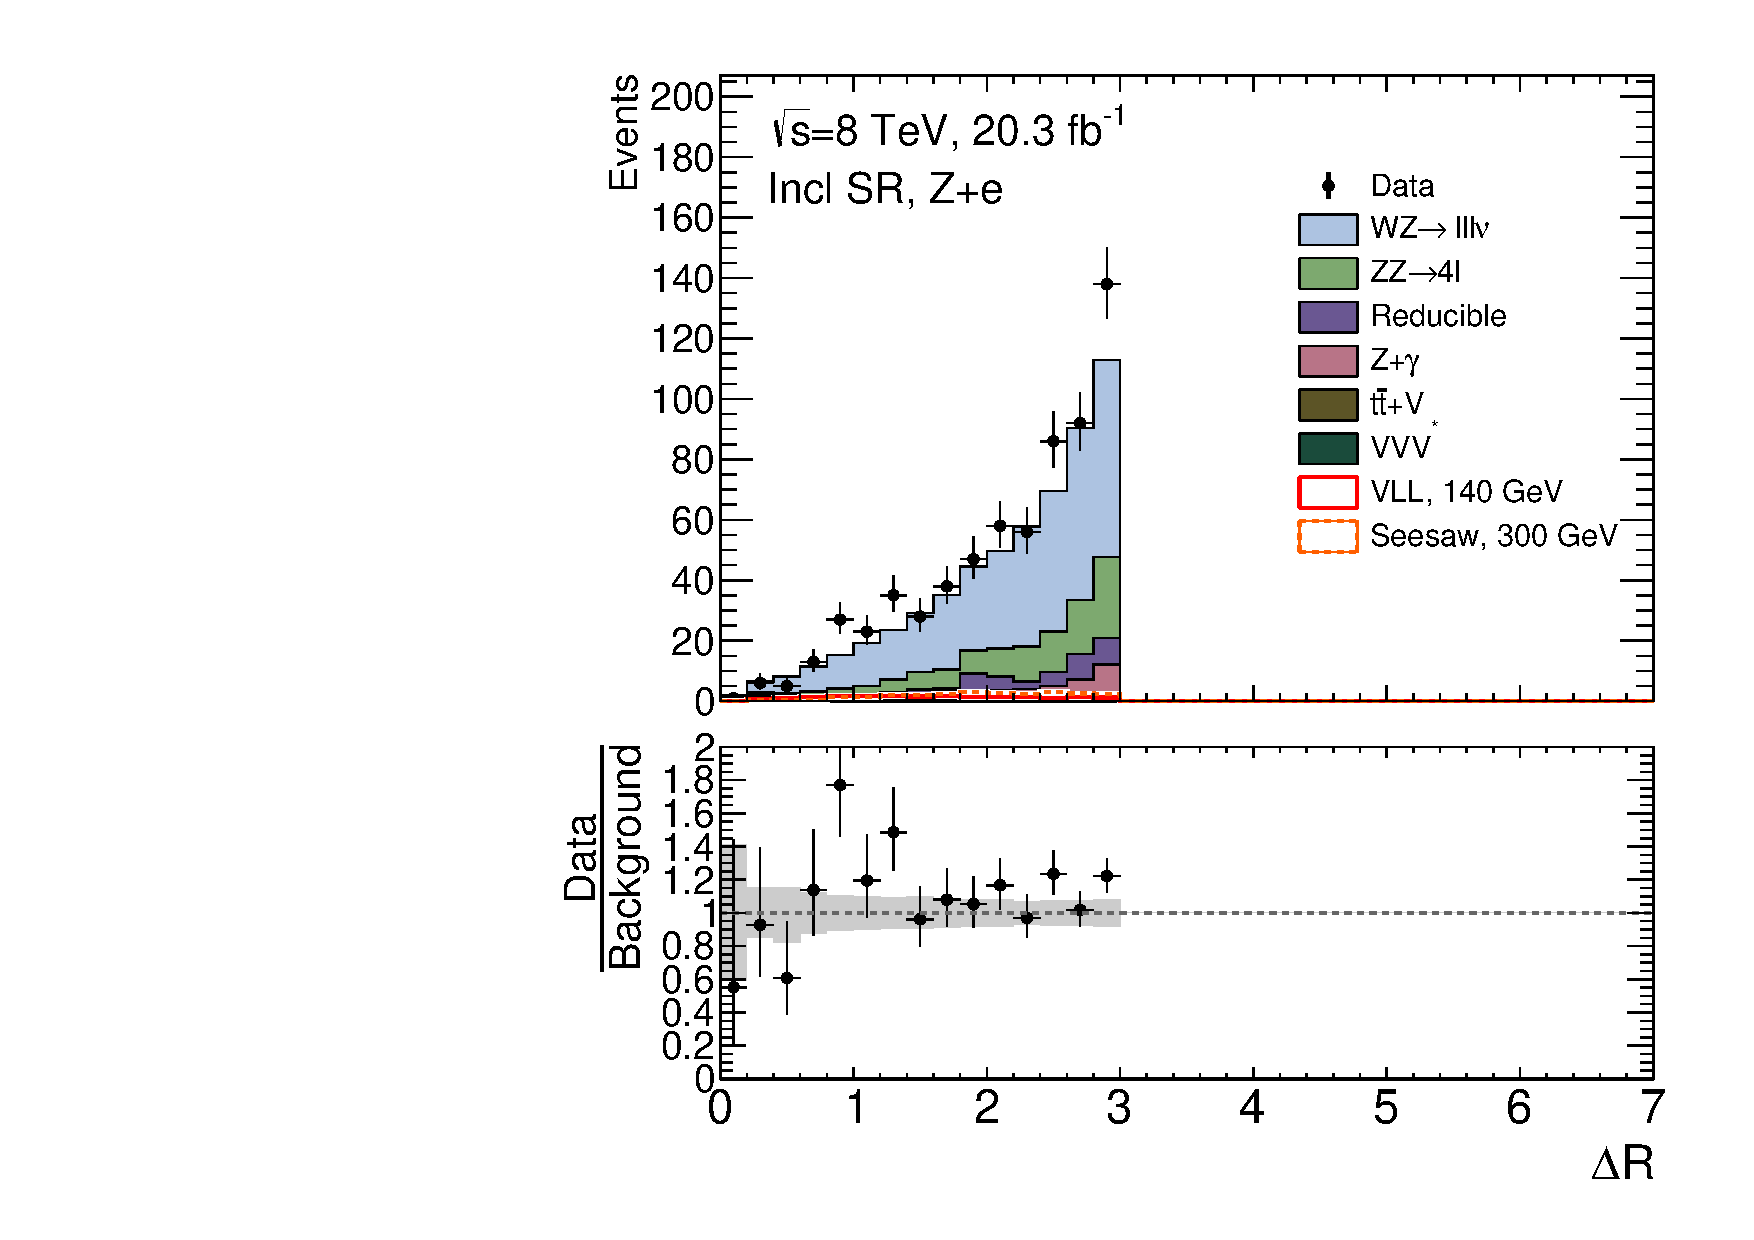
\includegraphics{figures/resonance/c_output_dR_Ze_InclusiveNoM3L_300GeV}}
  }
  \subfloat[ $Z+\mu$, inclusive] {
    \resizebox{0.48\textwidth}{!}{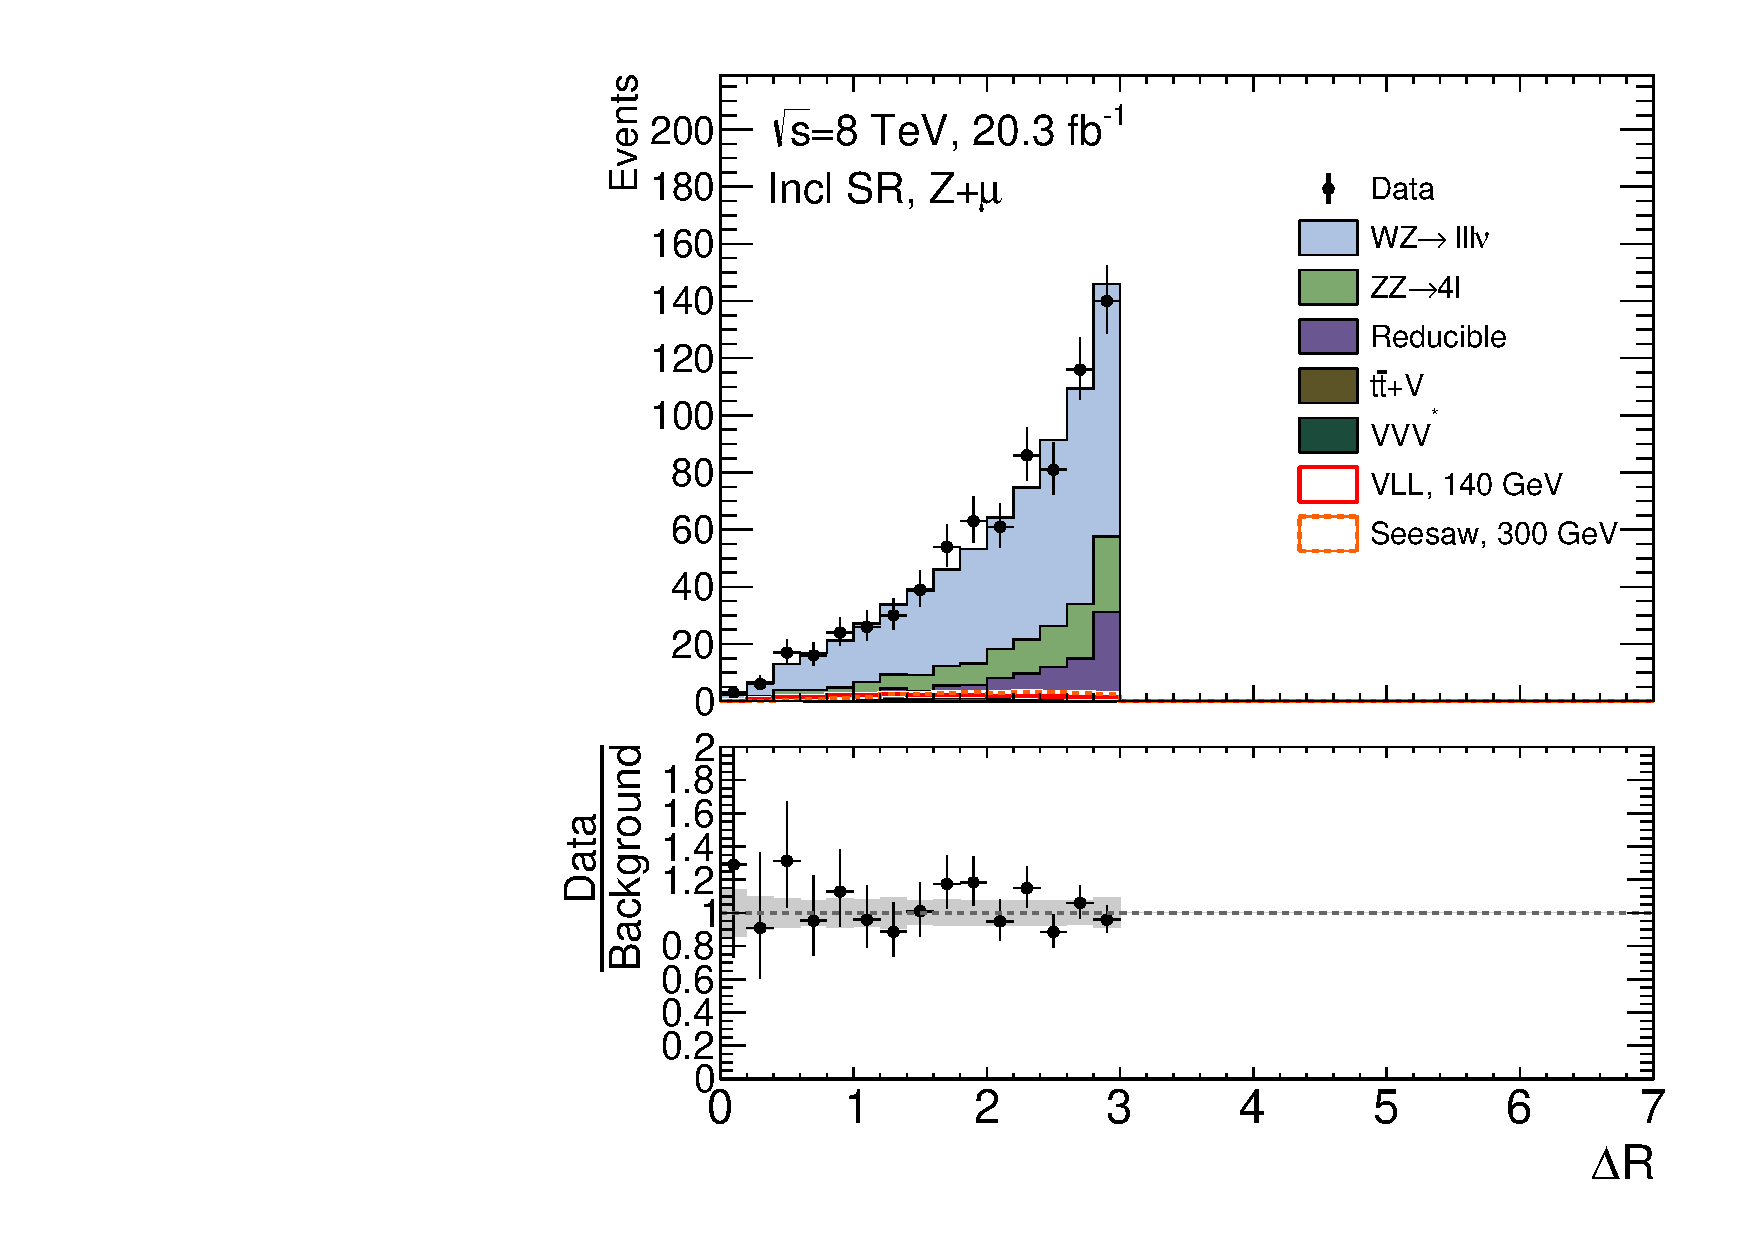
\includegraphics{figures/resonance/c_output_dR_Zmu_InclusiveNoM3L_300GeV}}
  } \\
  \subfloat[ $Z+e$, $4L$ category] {
    \resizebox{0.48\textwidth}{!}{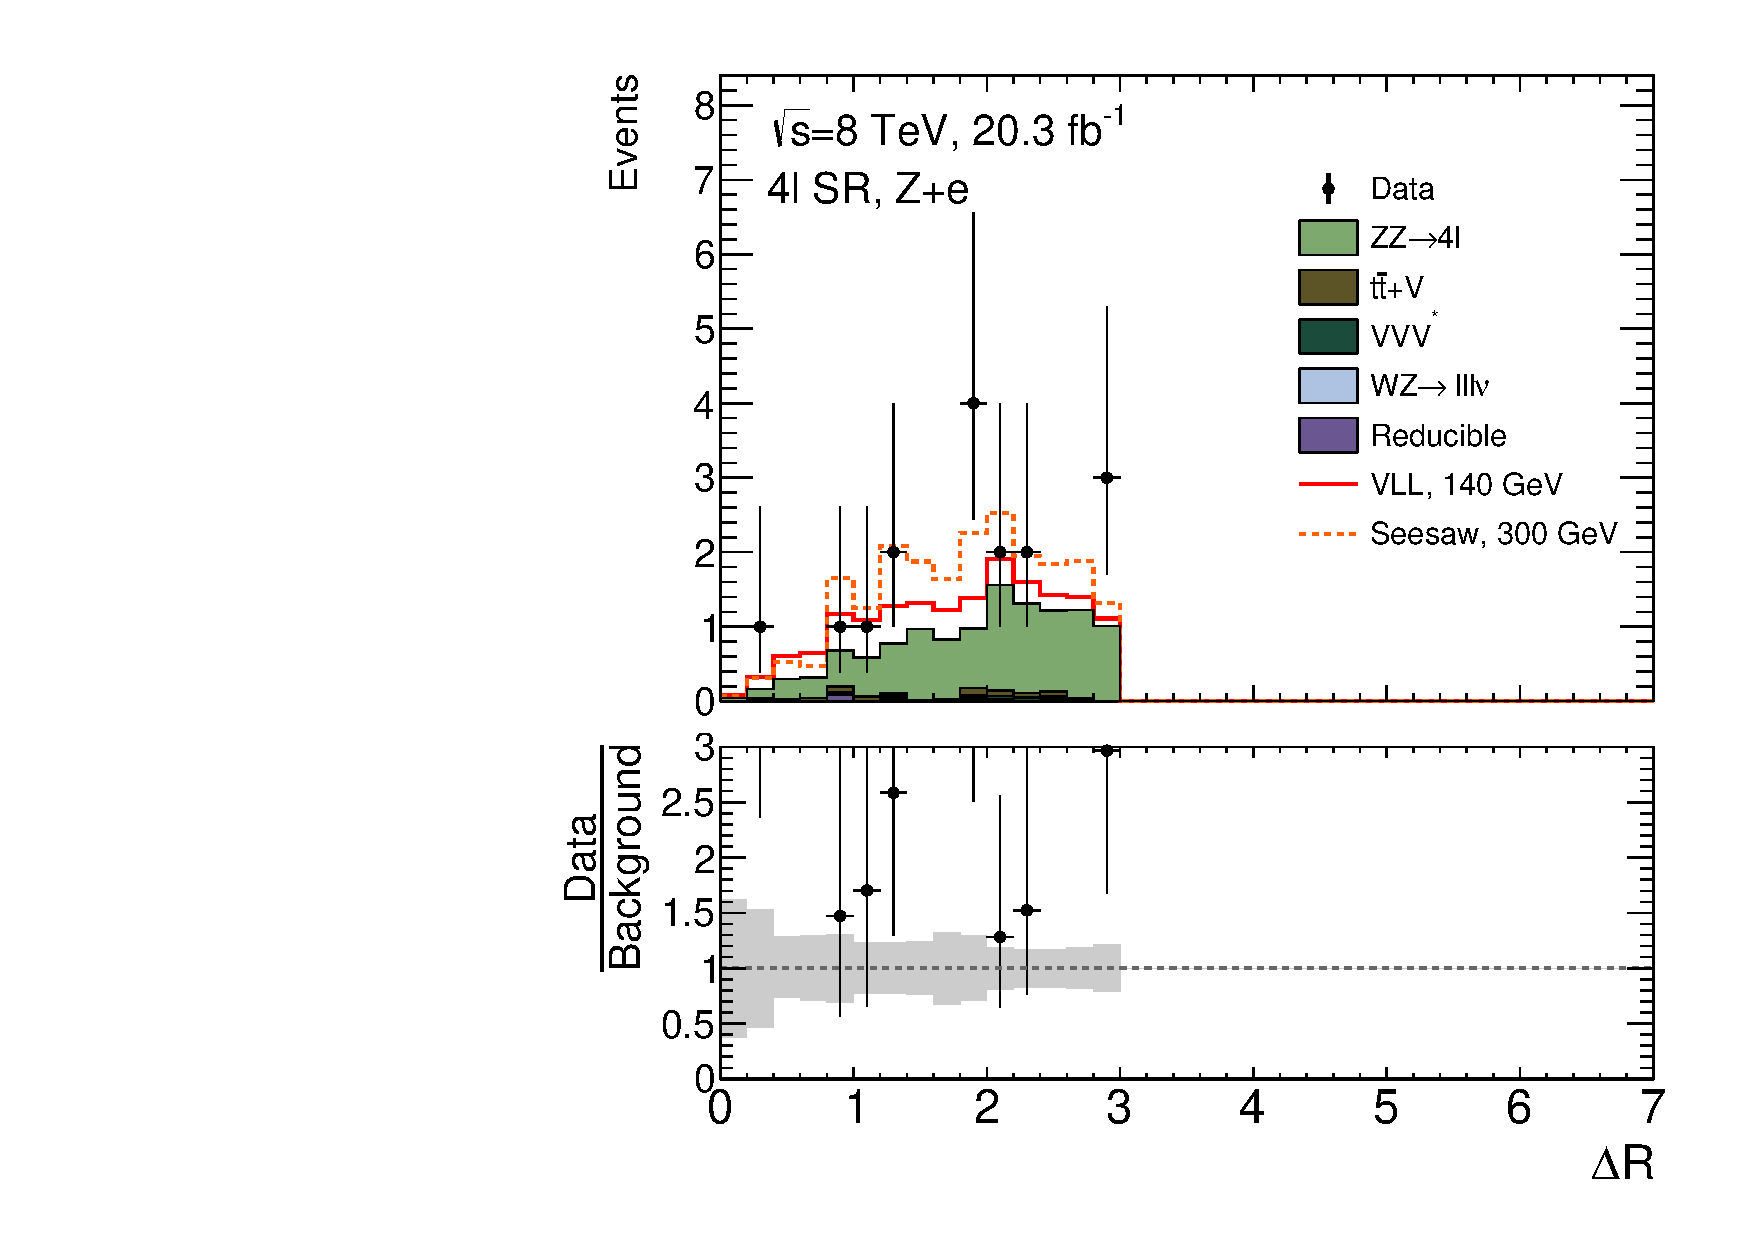
\includegraphics{figures/resonance/c_output_dR_Ze_FourLNoM3L_300GeV}}
  }
  \subfloat[ $Z+\mu$, $4L$ category] {
    \resizebox{0.48\textwidth}{!}{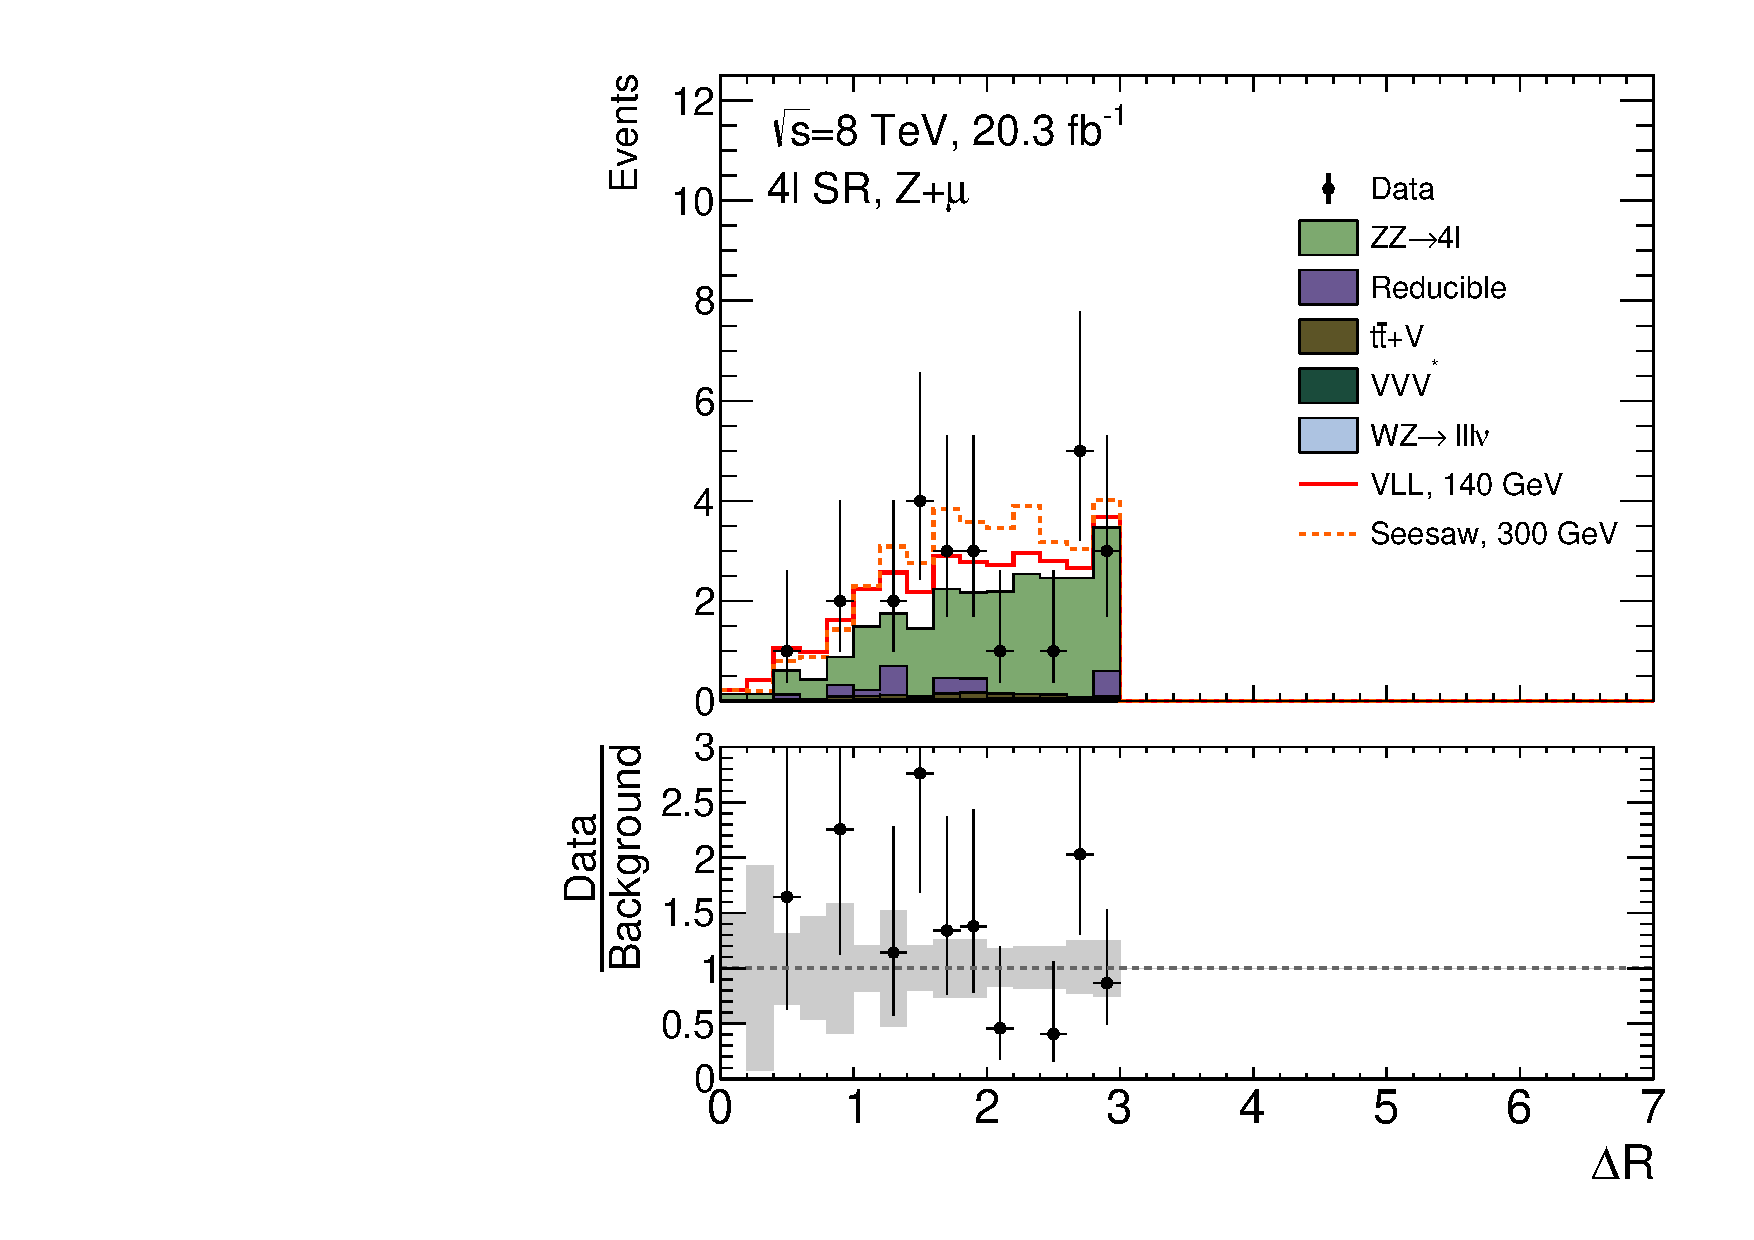
\includegraphics{figures/resonance/c_output_dR_Zmu_FourLNoM3L_300GeV}}
  } \\
  \caption{$\Delta R(Z,\ell_3)$ distributions for $Z+e$ and $Z+\mu$ candidates, for the inclusive and $\fourl$ signal regions (linear scale).}
  \label{fig:SR-dR-1-linear}
\end{figure}

\begin{figure}
  \centering
  \subfloat[ $Z+e$, dijet category] {
    \resizebox{0.48\textwidth}{!}{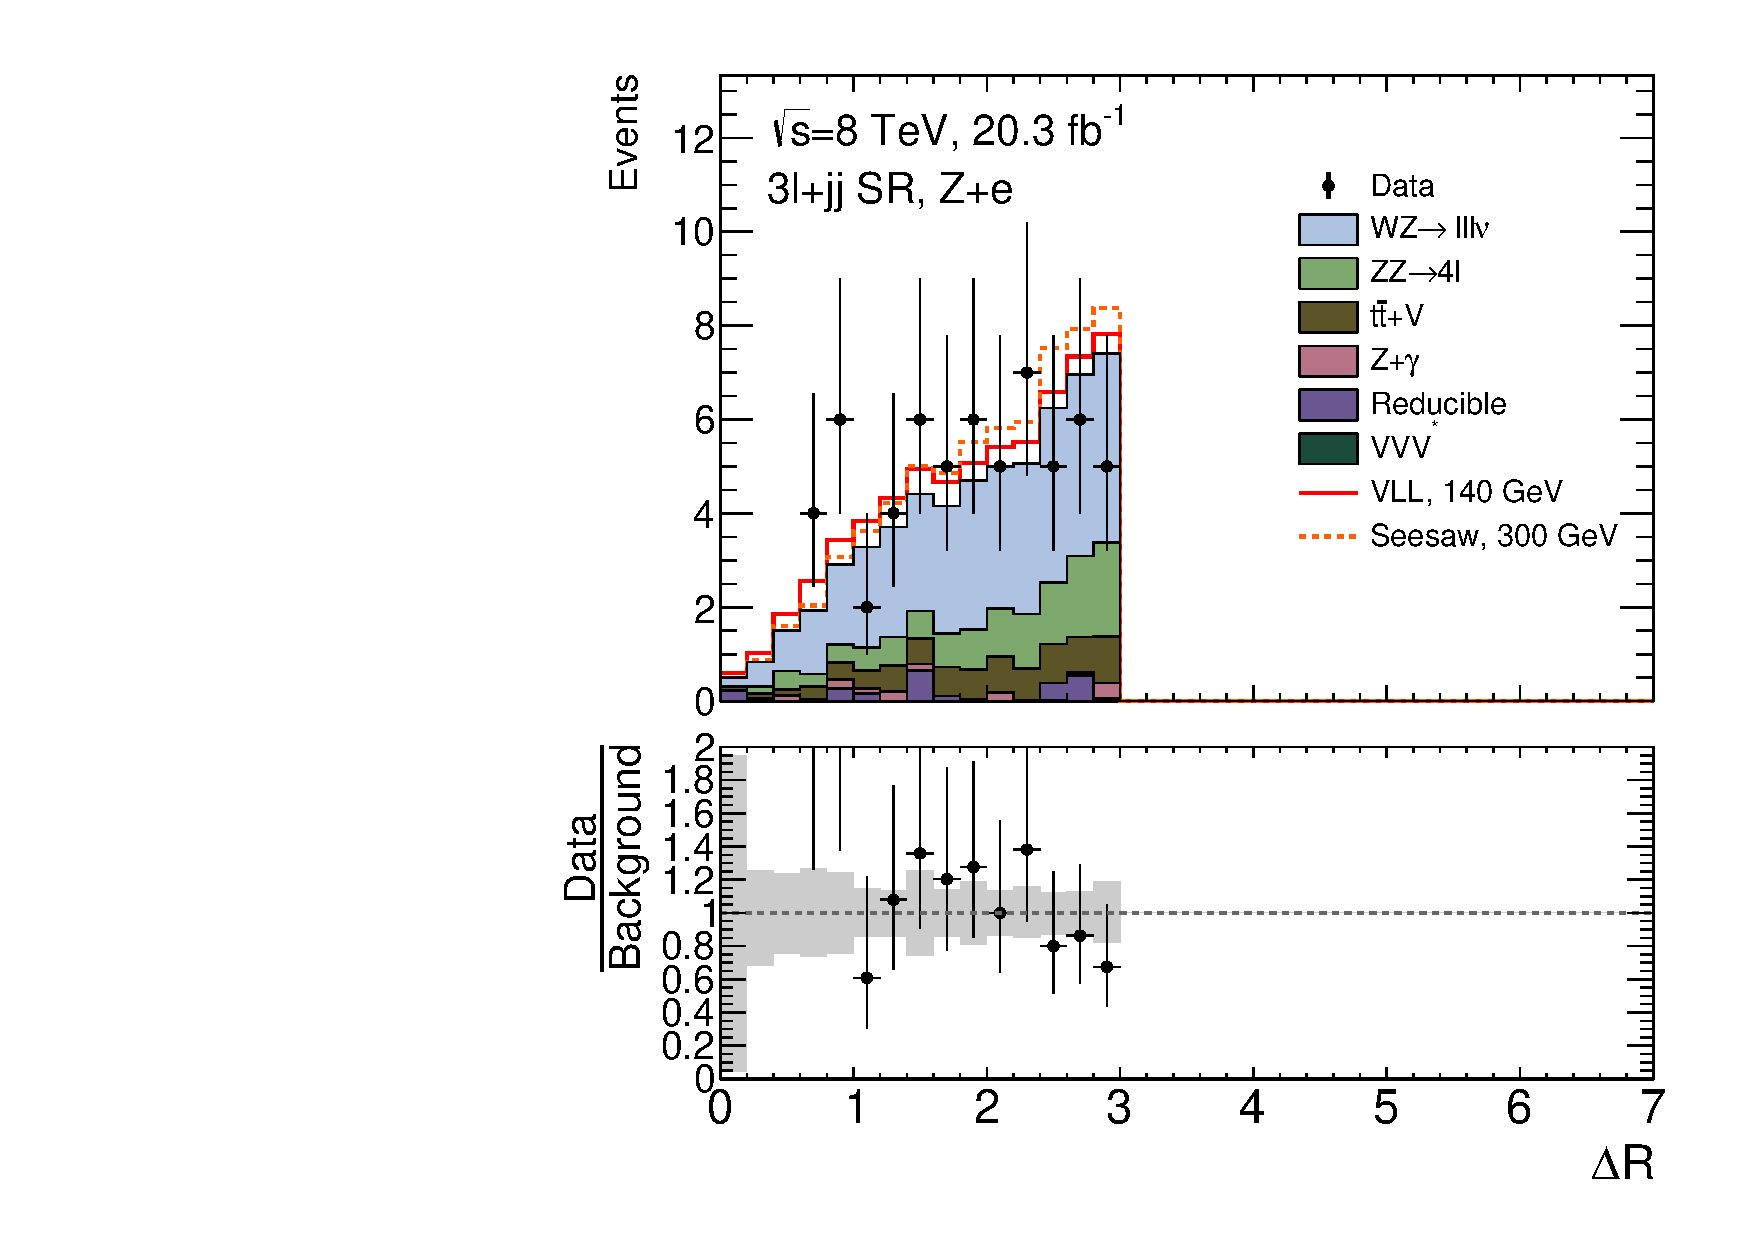
\includegraphics{figures/resonance/c_output_dR_Ze_ThreeLDijetNoM3L_300GeV}}
  }
  \subfloat[ $Z+\mu$, dijet category] {
    \resizebox{0.48\textwidth}{!}{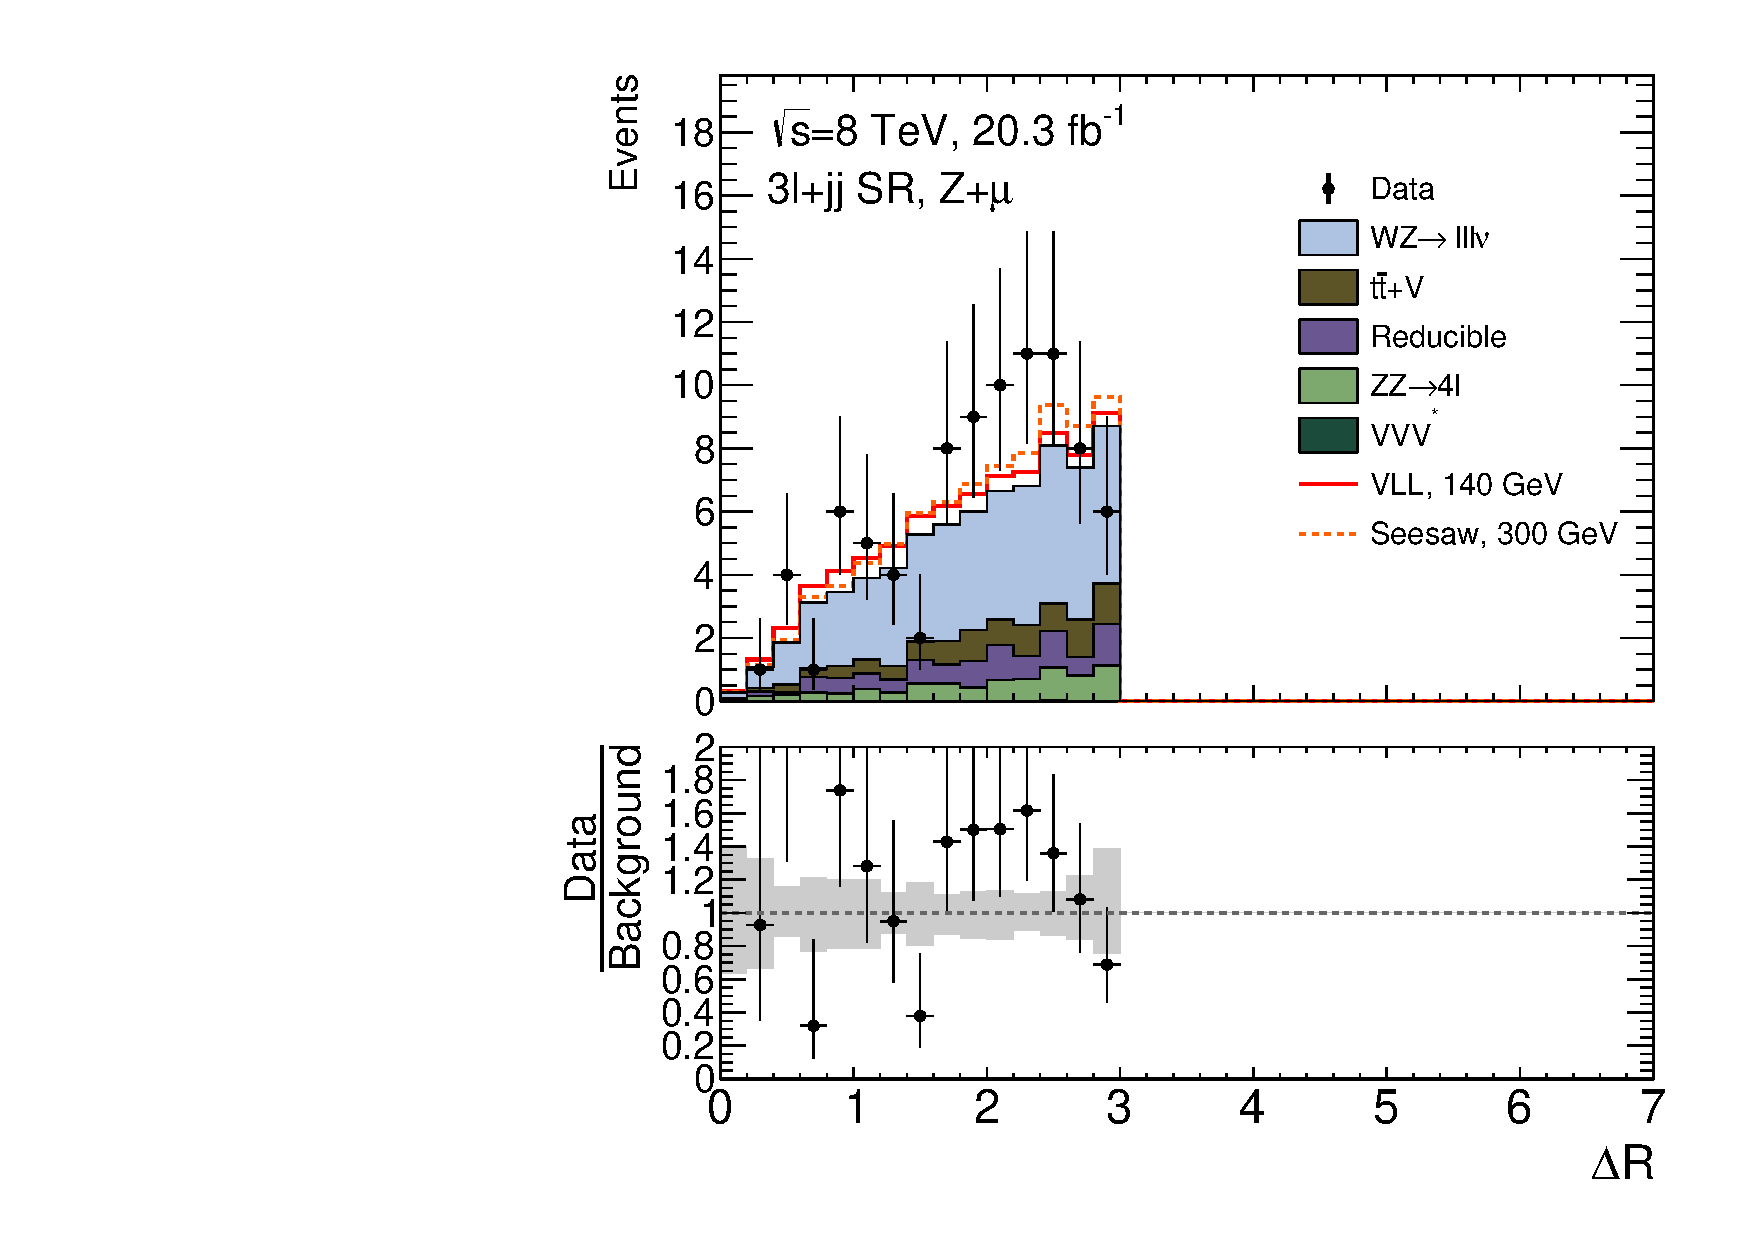
\includegraphics{figures/resonance/c_output_dR_Zmu_ThreeLDijetNoM3L_300GeV}}
  } \\
  \subfloat[ $Z+e$, else category] {
    \resizebox{0.48\textwidth}{!}{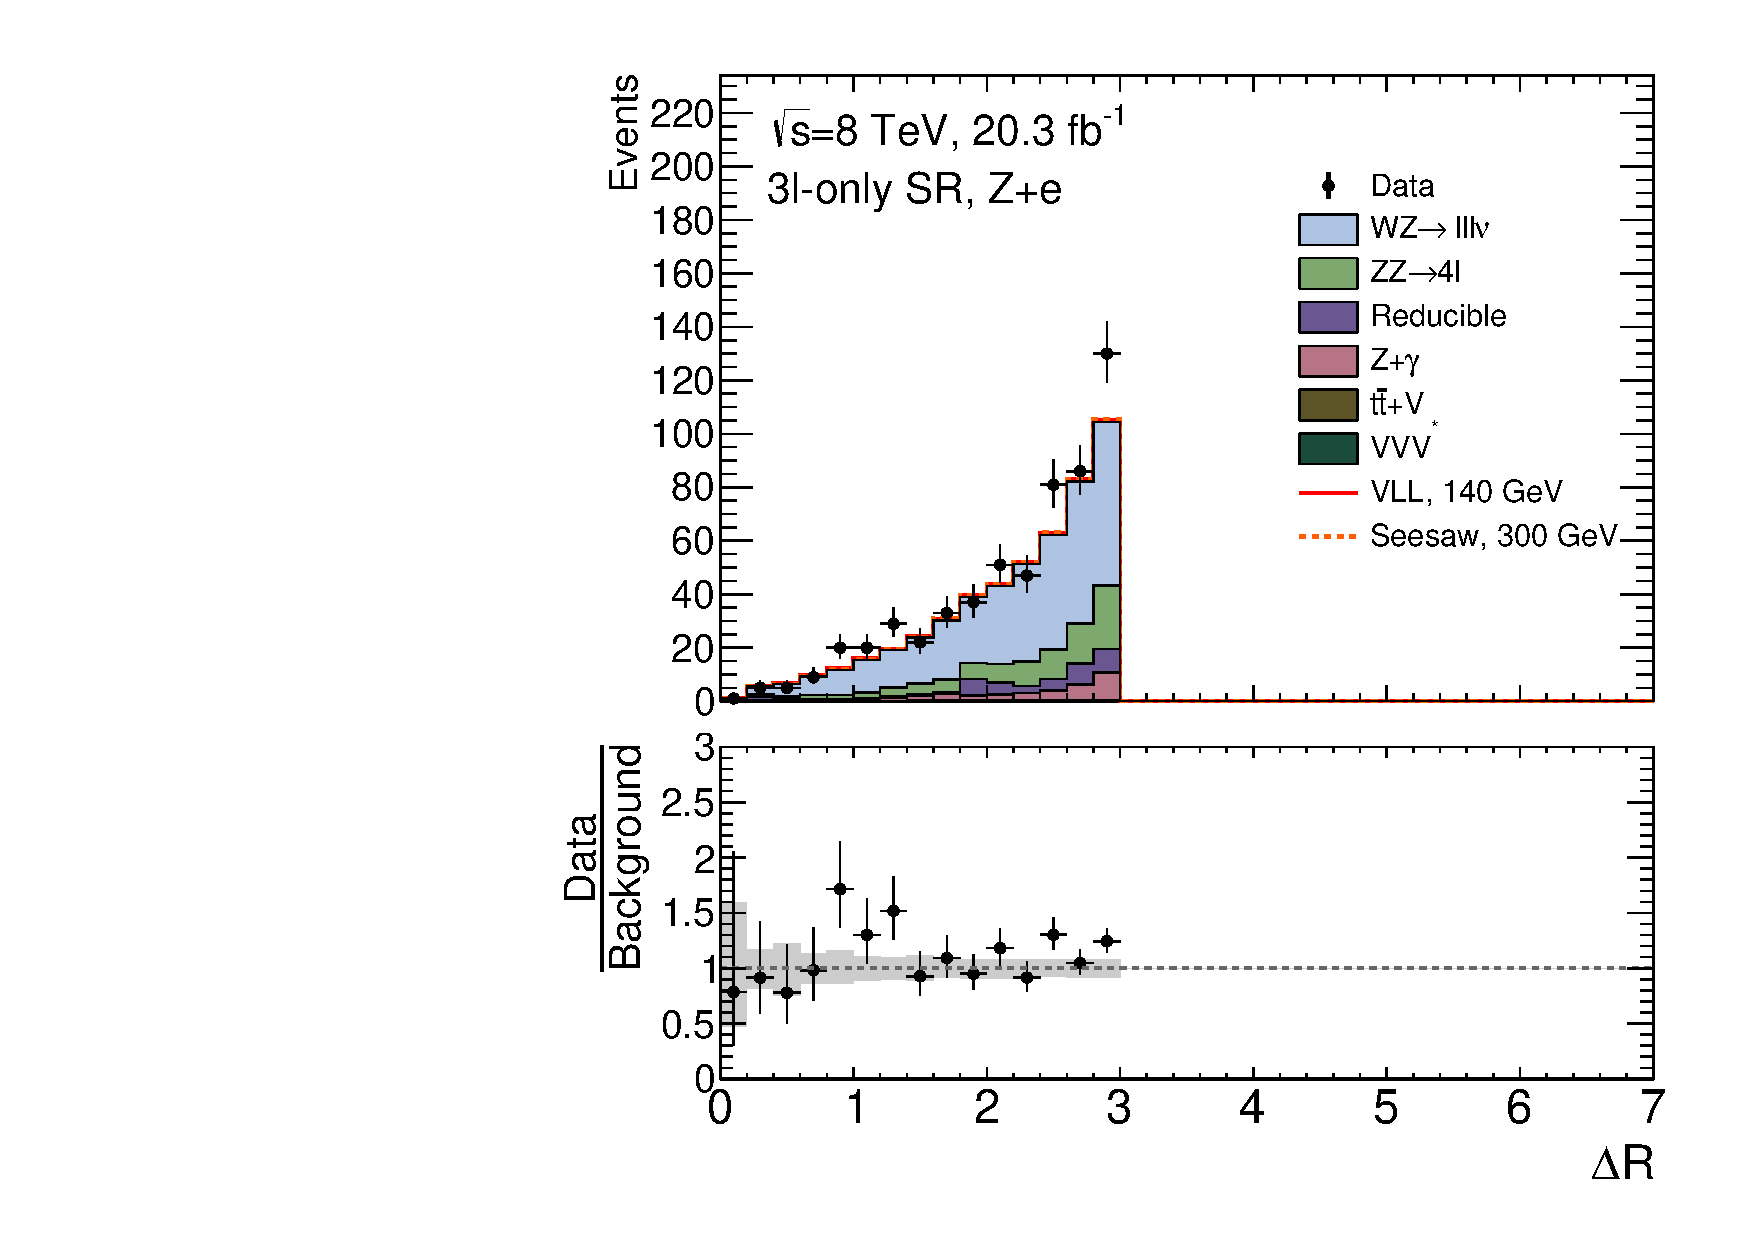
\includegraphics{figures/resonance/c_output_dR_Ze_ElseNoM3L_300GeV}}
  }
  \subfloat[ $Z+\mu$, else category] {
    \resizebox{0.48\textwidth}{!}{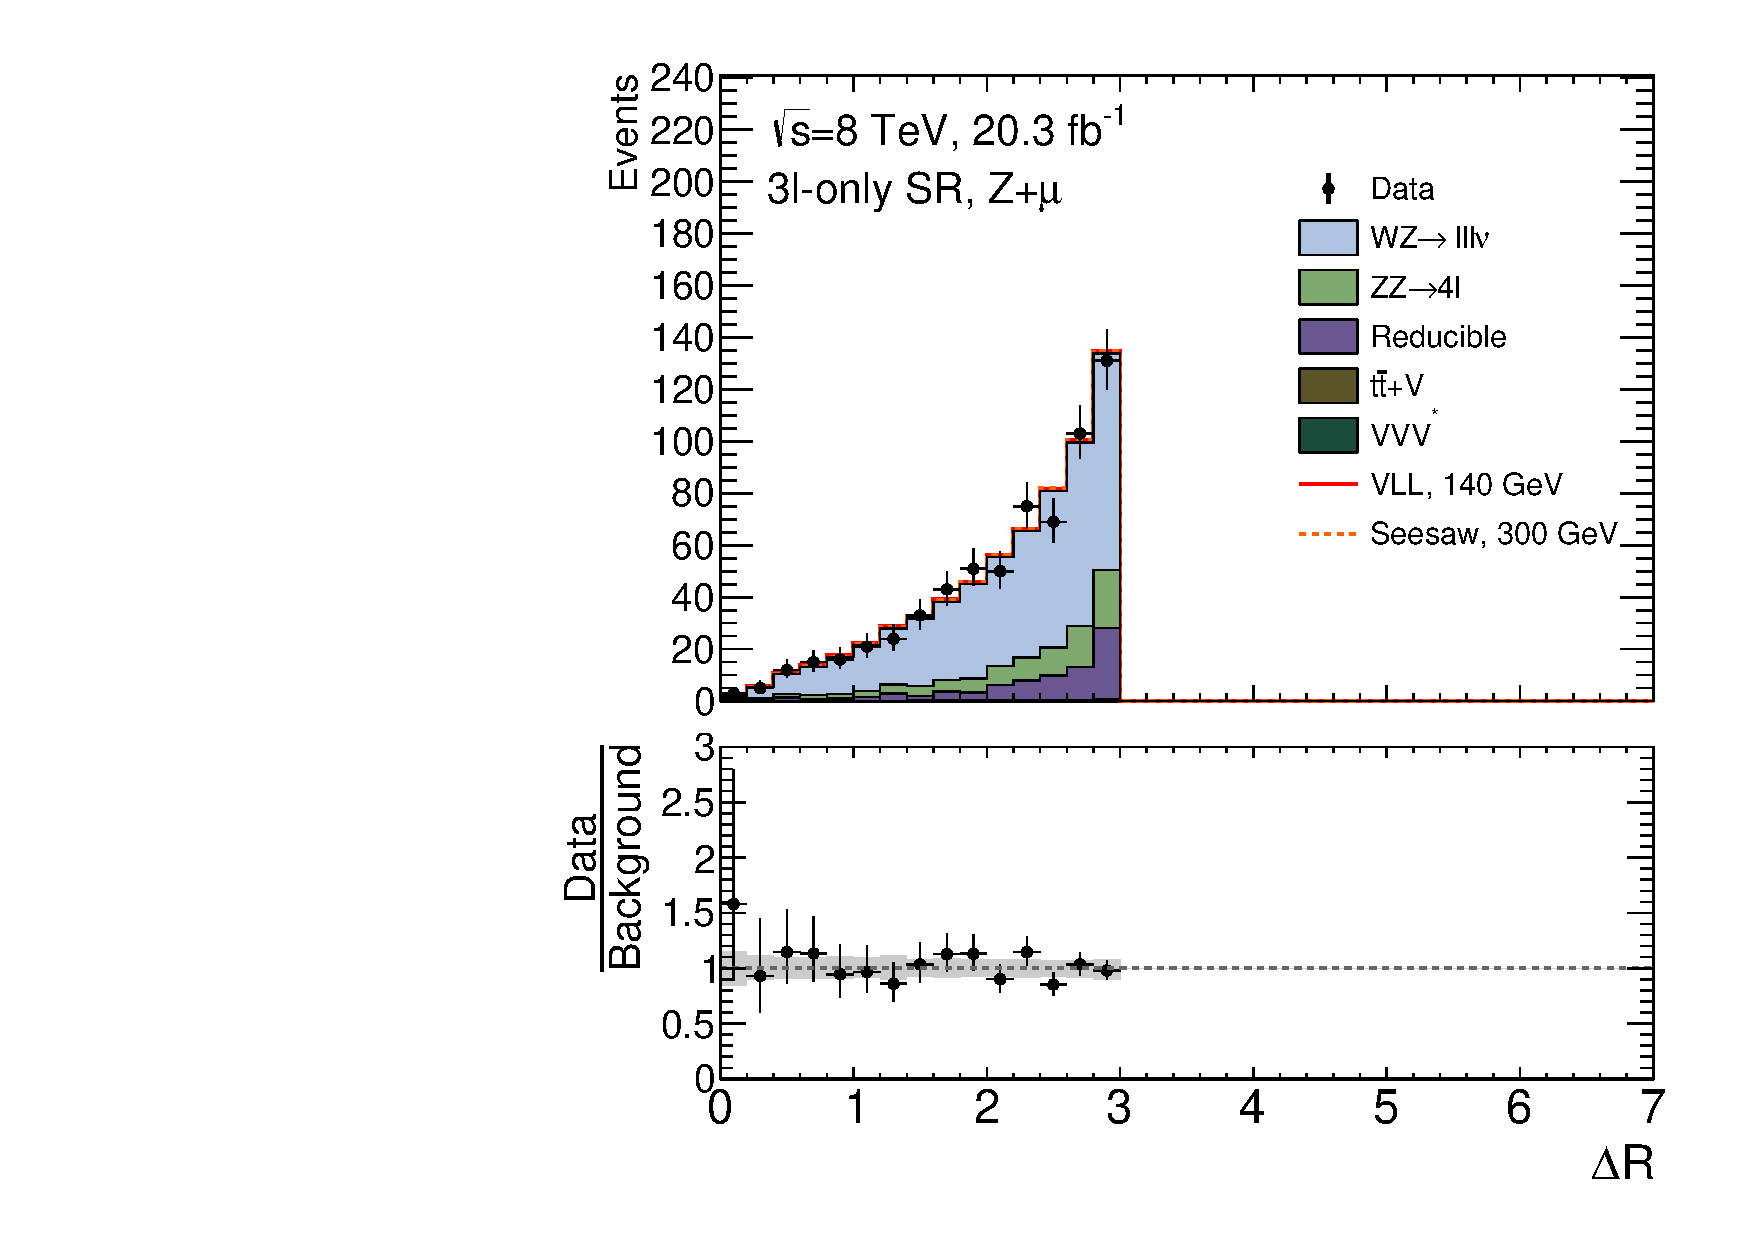
\includegraphics{figures/resonance/c_output_dR_Zmu_ElseNoM3L_300GeV}}
  }
  \caption{$\Delta R(Z,\ell_3)$ distributions for $Z+e$ and $Z+\mu$ candidates, for the $\threeljj$ and $\threelo$ signal regions (linear scale).}
  \label{fig:SR-dR-2-linear}
\end{figure}


\begin{figure}[htb]
  \centering
  \subfloat[ $Z+e$, inclusive] {
    \resizebox{0.48\textwidth}{!}{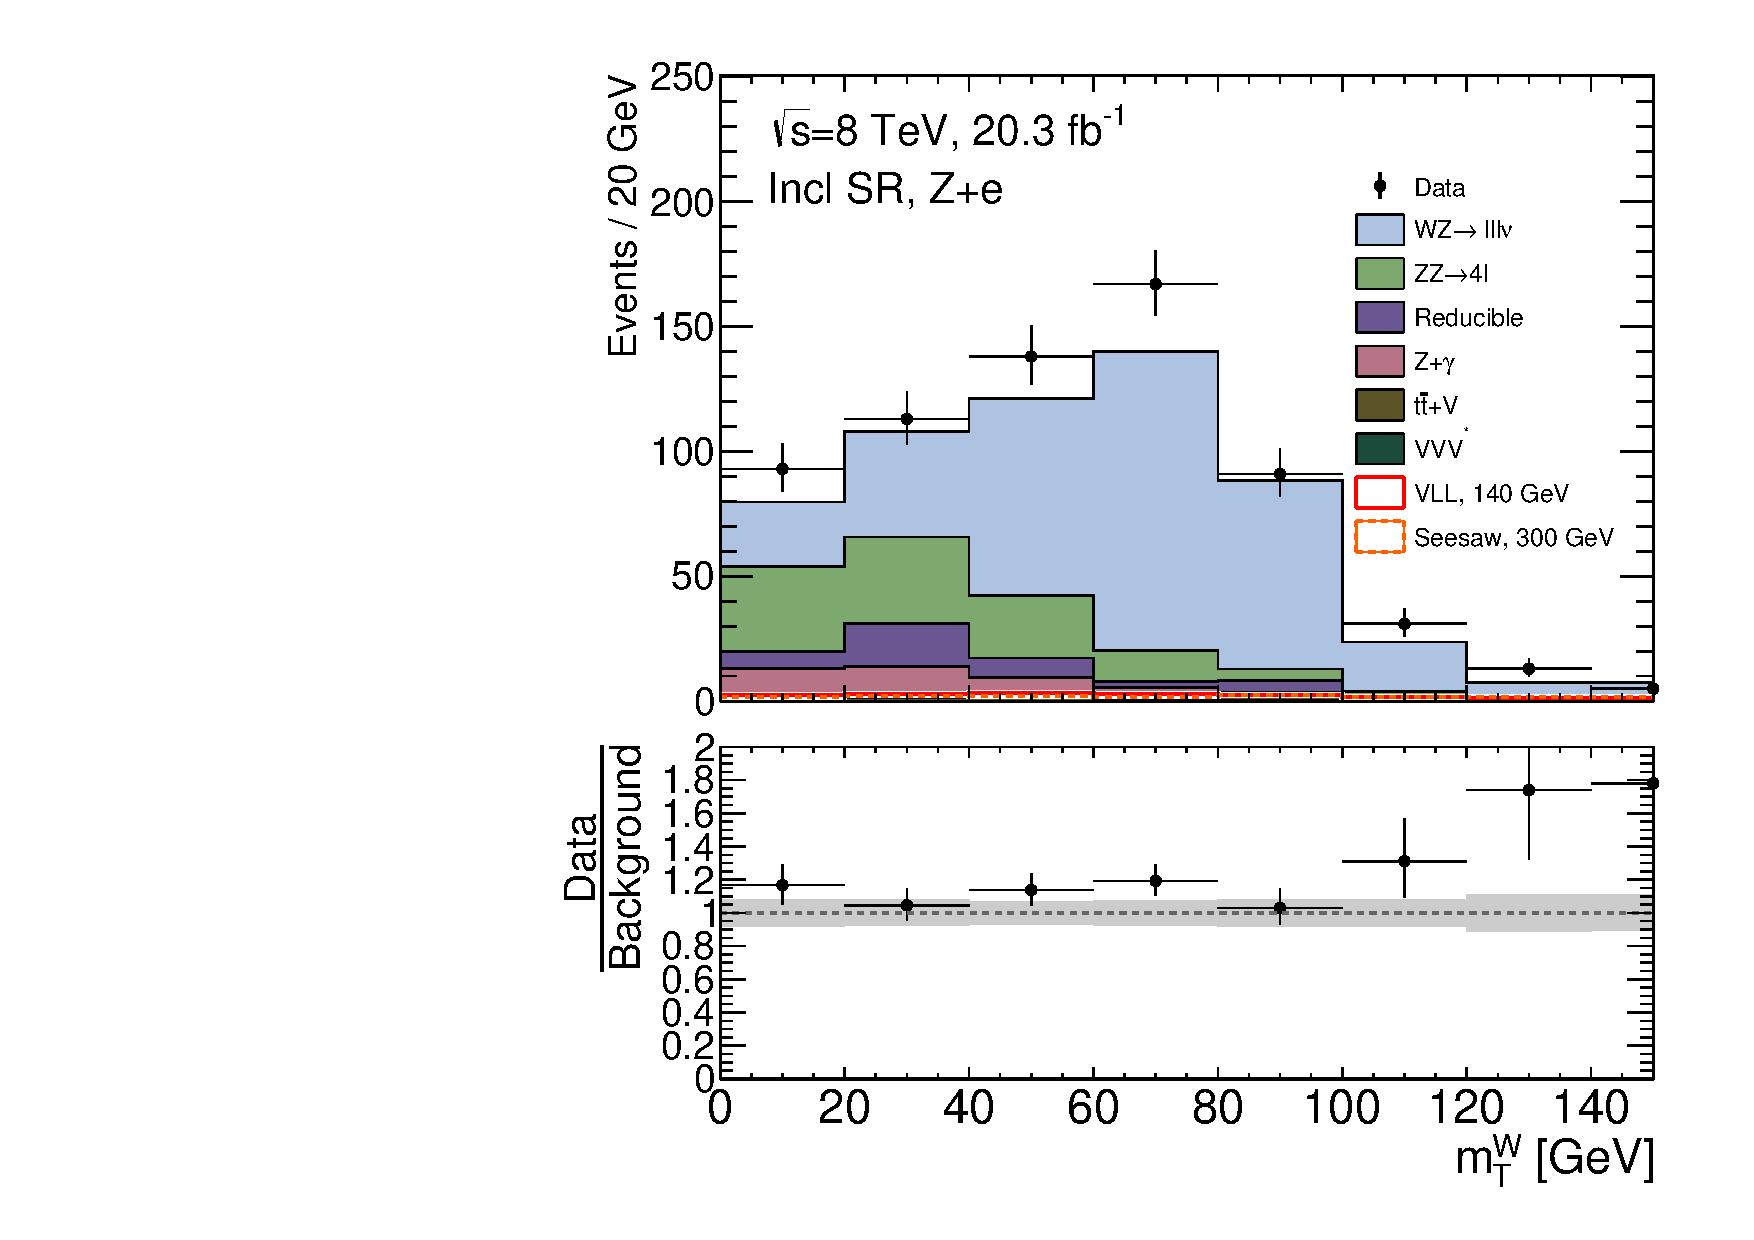
\includegraphics{figures/resonance/c_output_mTW_Ze_InclusiveNoM3L_300GeV}}
  }
  \subfloat[ $Z+\mu$, inclusive] {
    \resizebox{0.48\textwidth}{!}{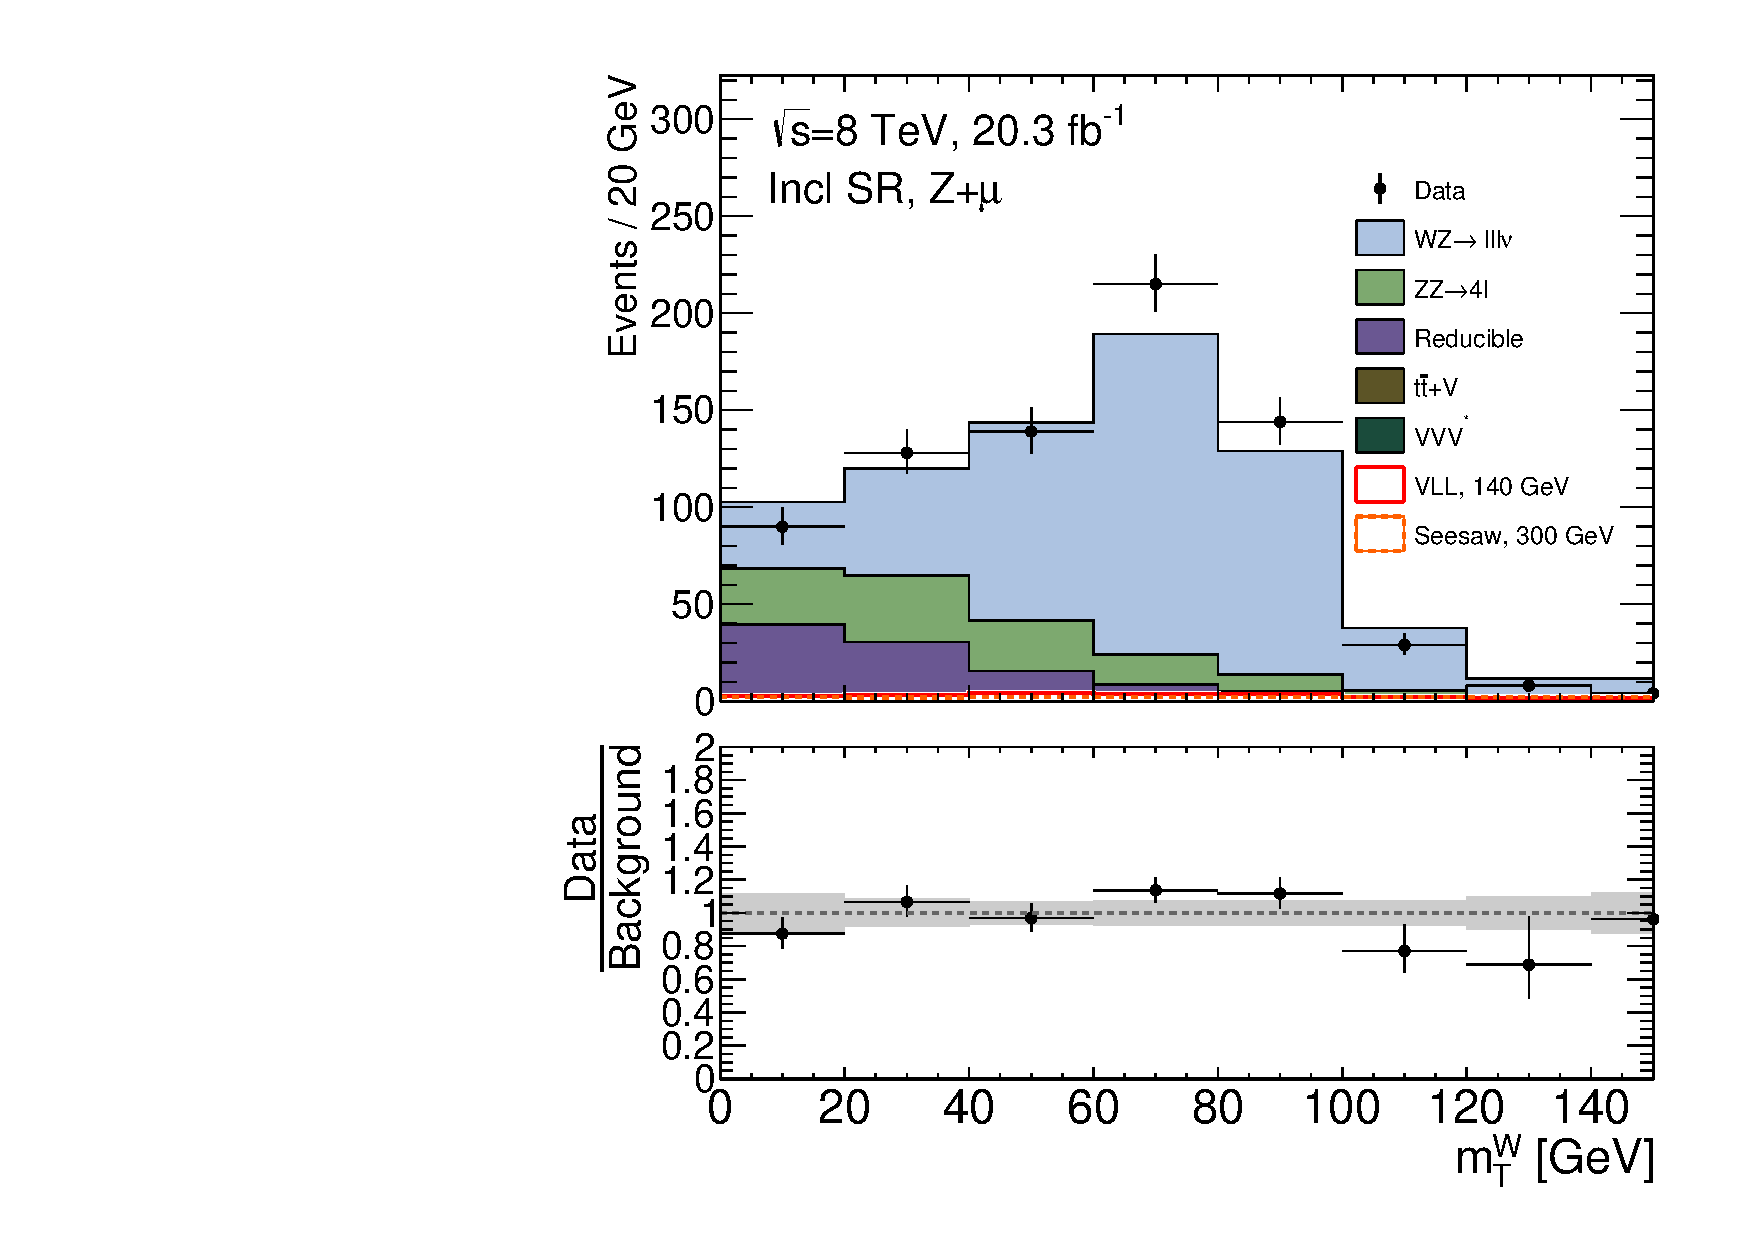
\includegraphics{figures/resonance/c_output_mTW_Zmu_InclusiveNoM3L_300GeV}}
  } \\
  \subfloat[ $Z+e$, $4L$ category] {
    \resizebox{0.48\textwidth}{!}{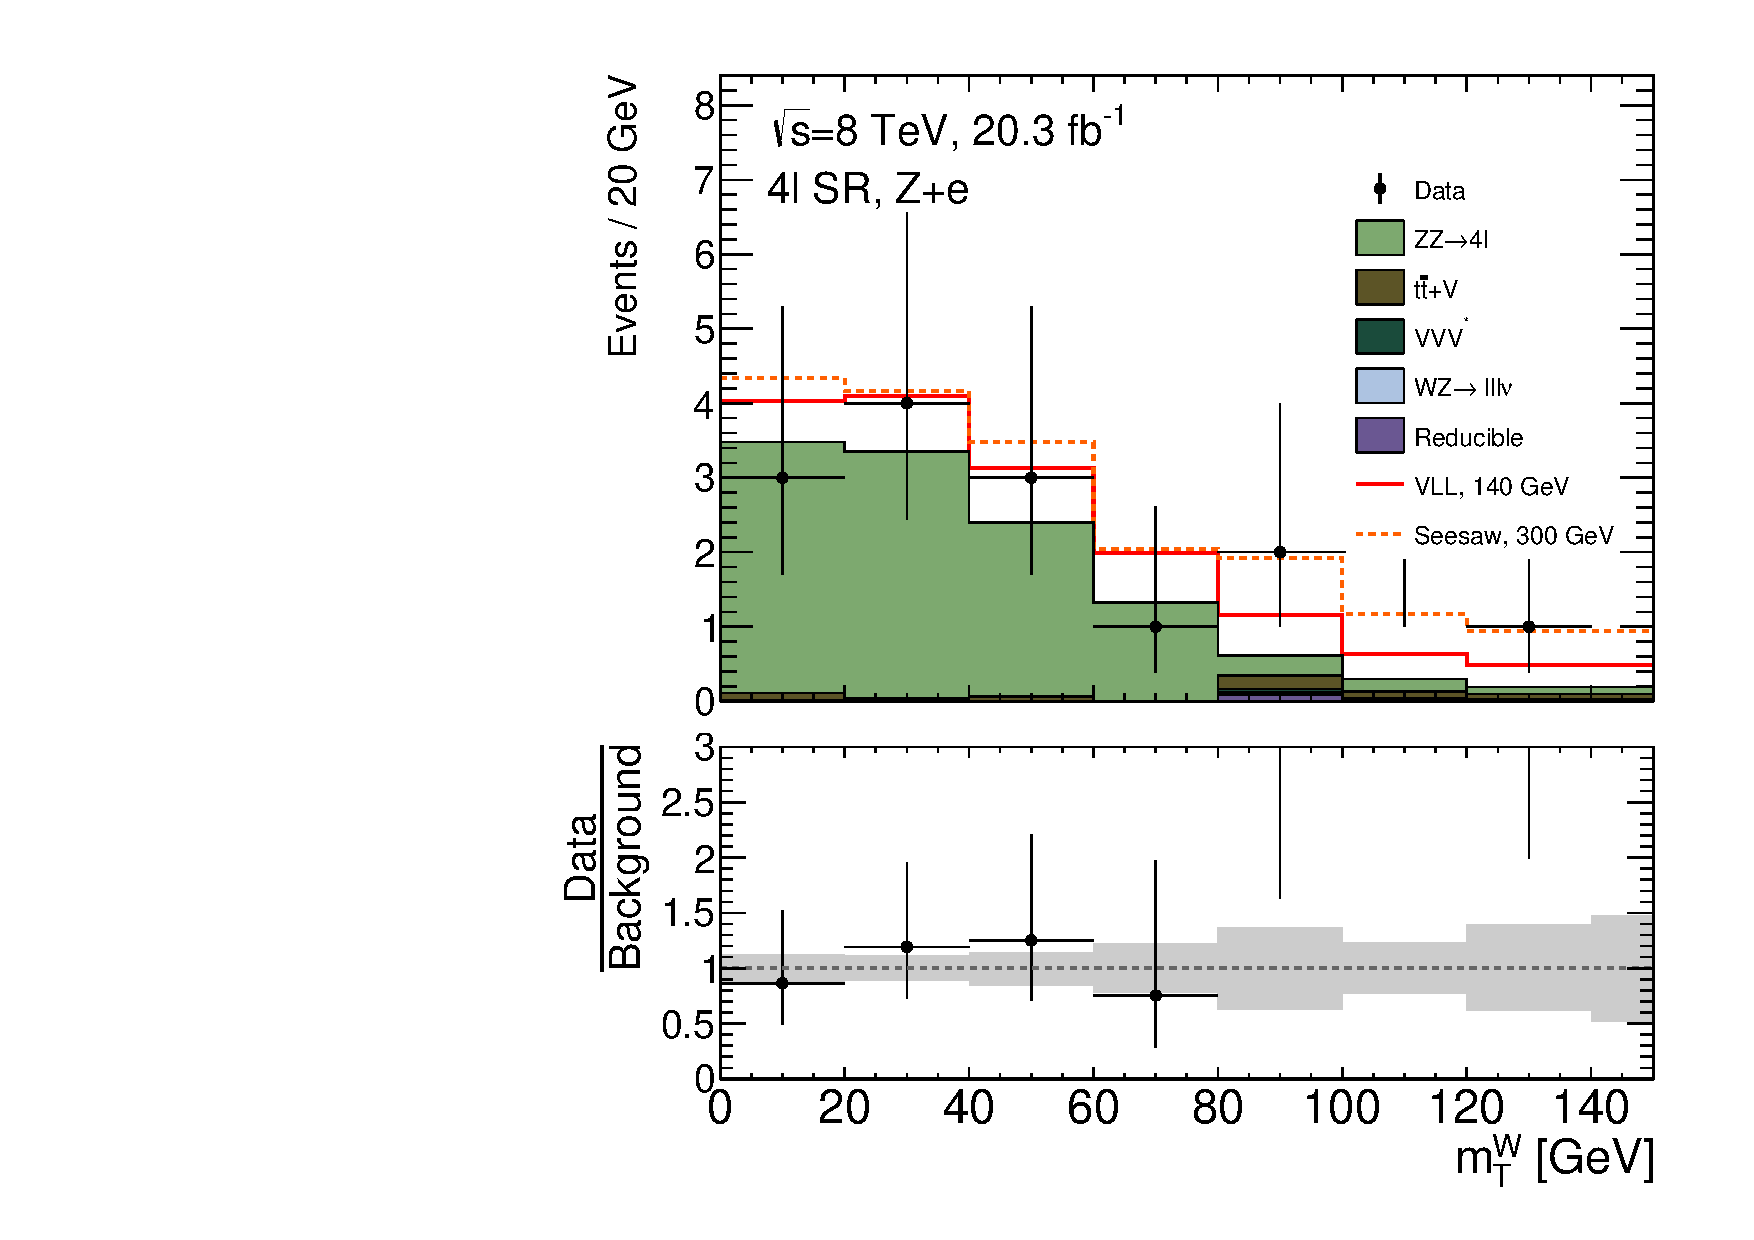
\includegraphics{figures/resonance/c_output_mTW_Ze_FourLNoM3L_300GeV}}
  }
  \subfloat[ $Z+\mu$, $4L$ category] {
    \resizebox{0.48\textwidth}{!}{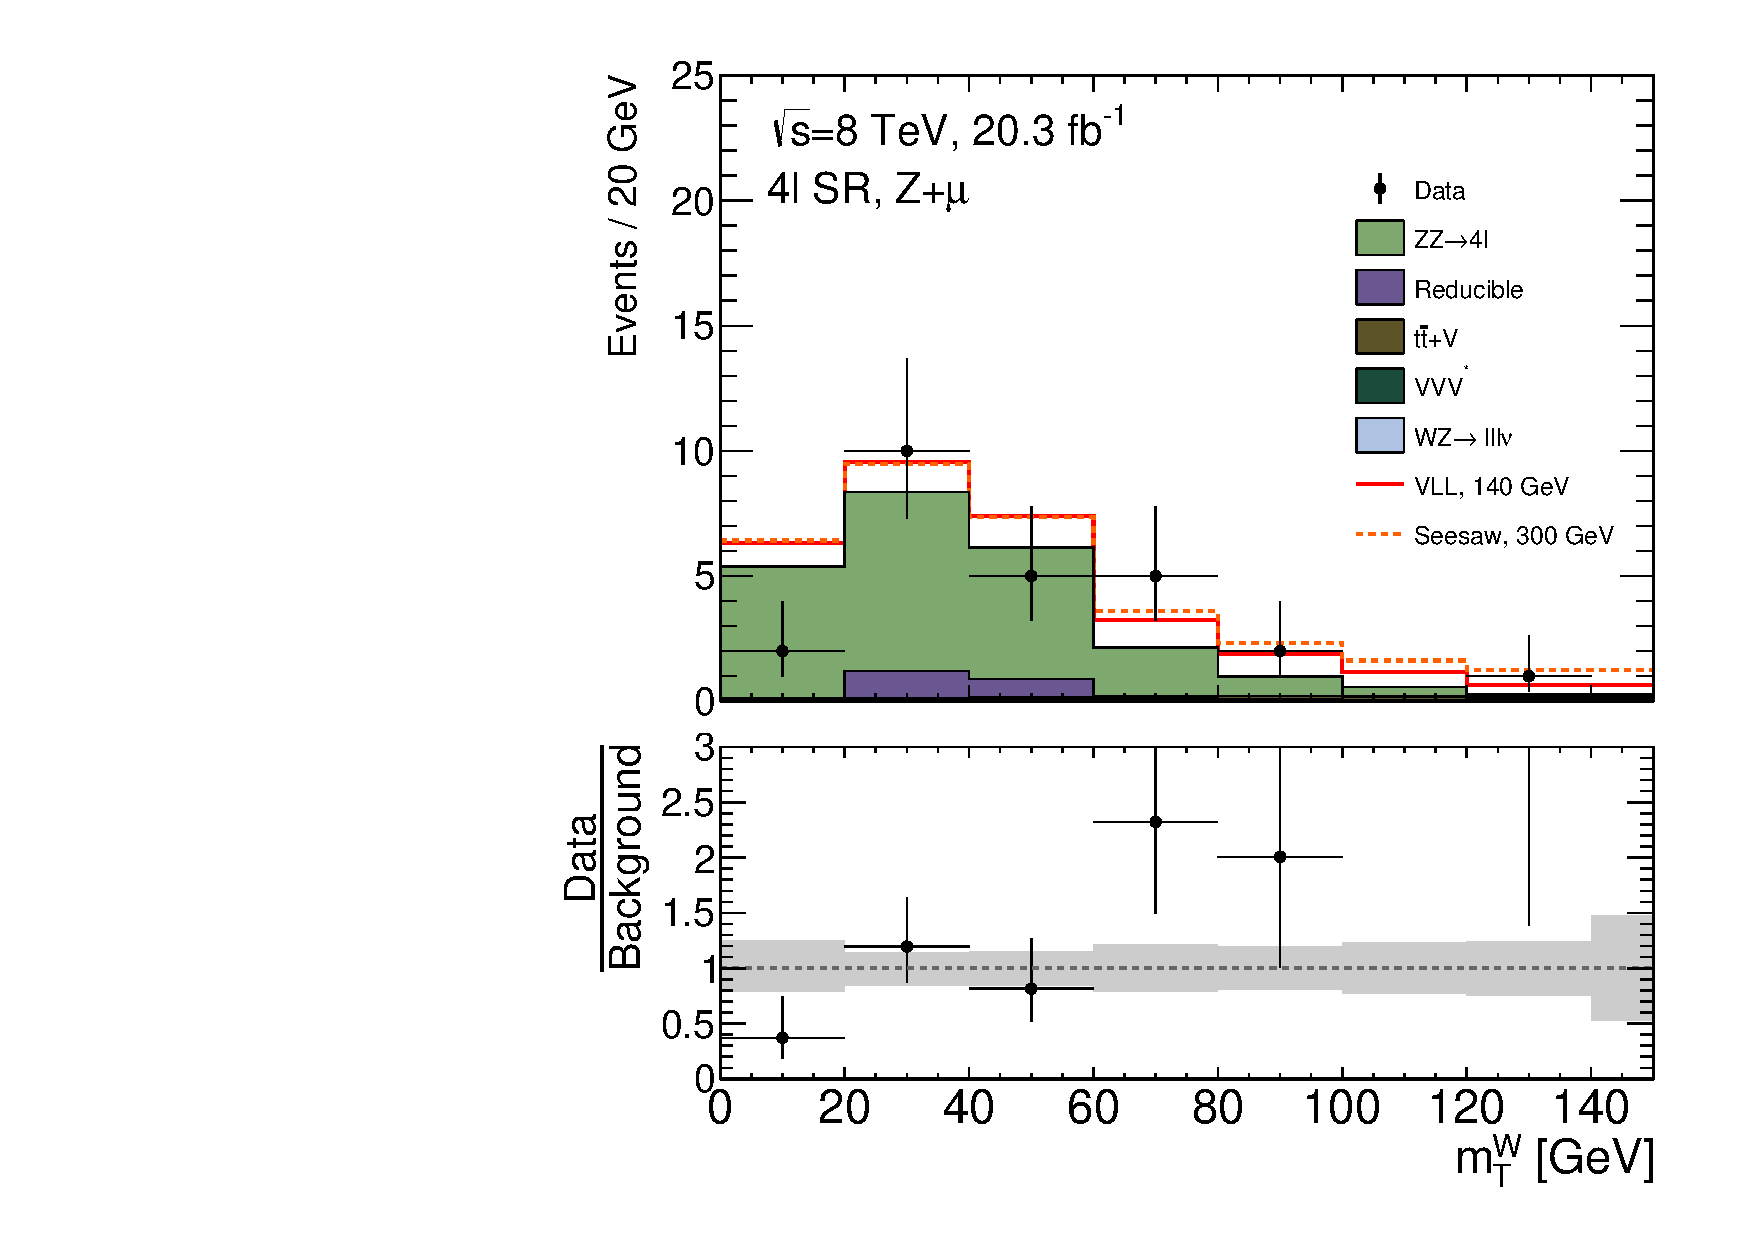
\includegraphics{figures/resonance/c_output_mTW_Zmu_FourLNoM3L_300GeV}}
  } \\
  \caption{Transverse mass of the missing energy and bachelor lepton ($\mtw$) for $Z+e$ and $Z+\mu$ candidates, for the inclusive and $\fourl$ signal regions.}
  \label{fig:SR-mTW-1}
\end{figure}

\clearpage

\begin{figure}[htb]
  \centering
  \subfloat[ $Z+e$, dijet category] {
    \resizebox{0.48\textwidth}{!}{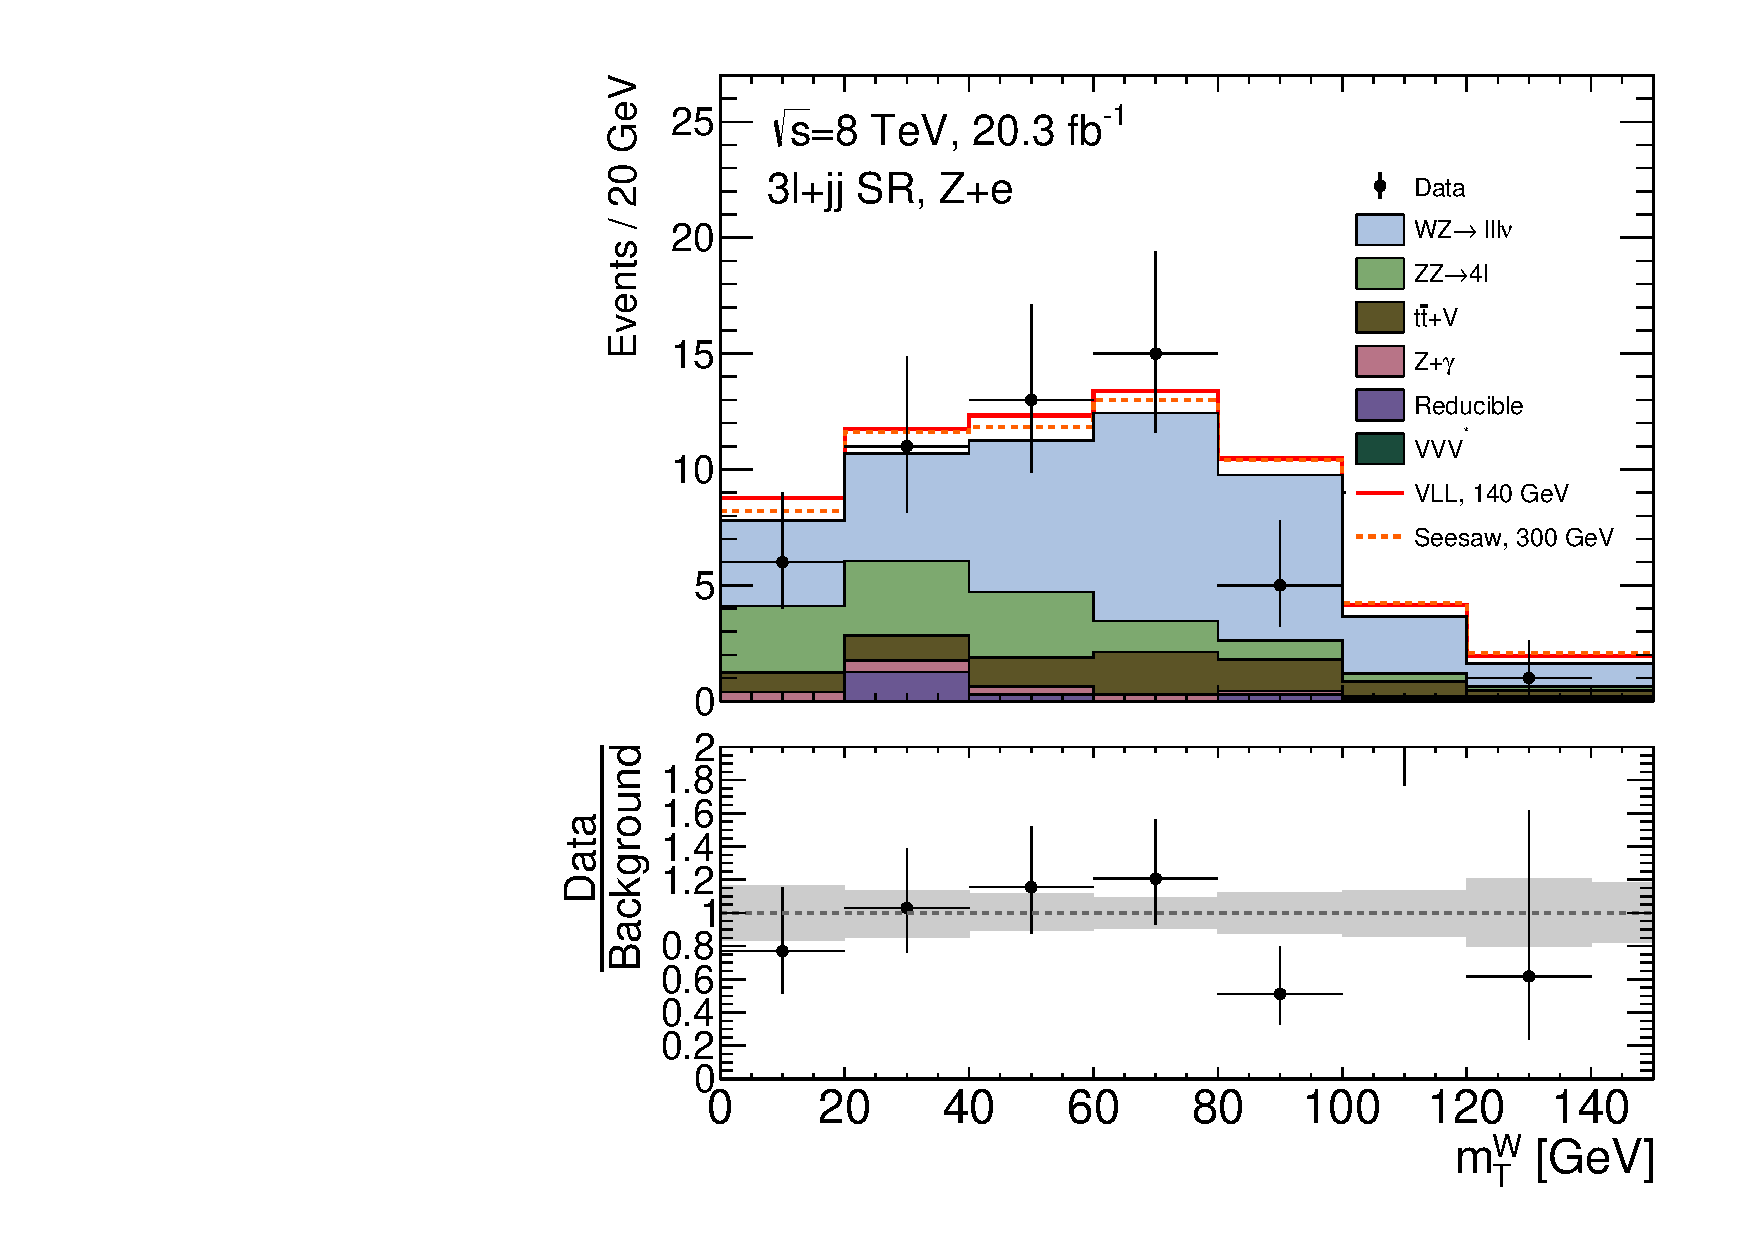
\includegraphics{figures/resonance/c_output_mTW_Ze_ThreeLDijetNoM3L_300GeV}}
  }
  \subfloat[ $Z+\mu$, dijet category] {
    \resizebox{0.48\textwidth}{!}{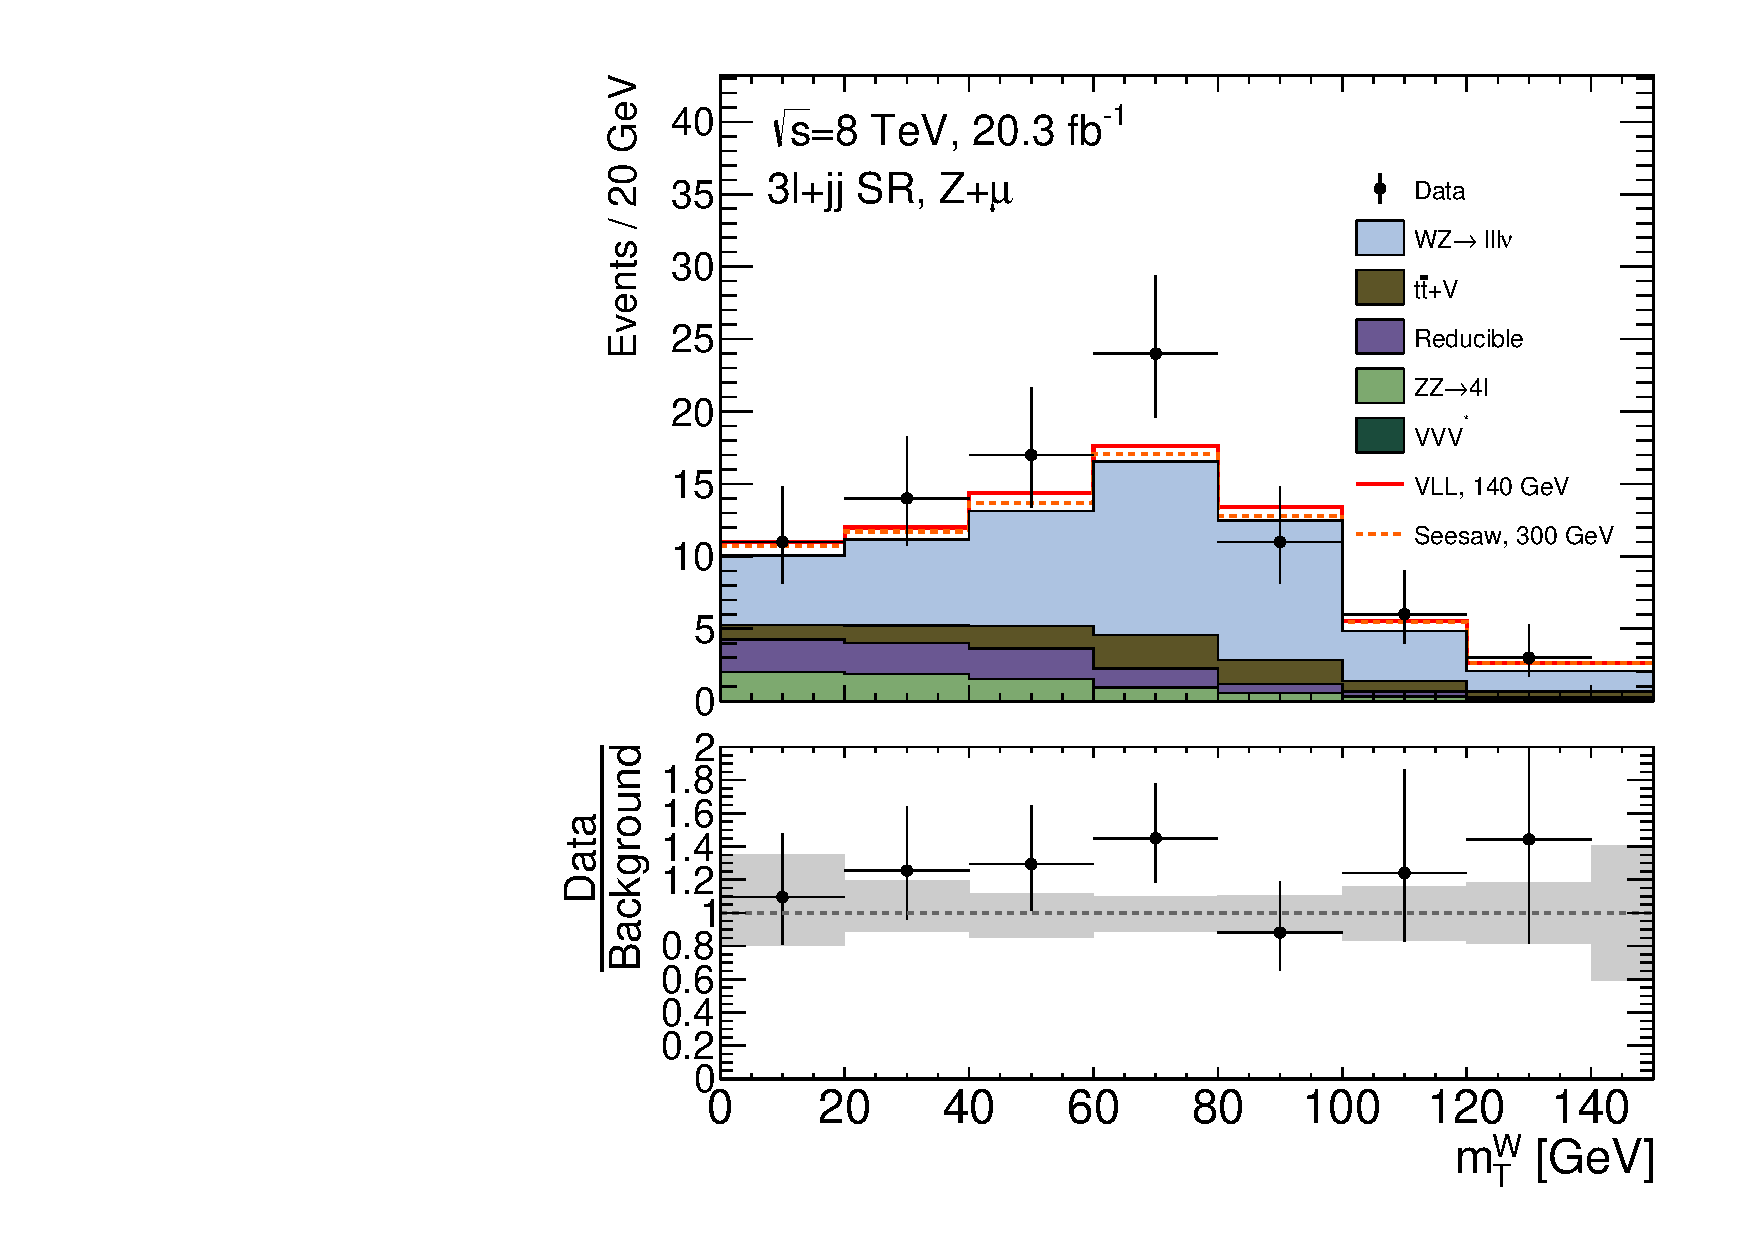
\includegraphics{figures/resonance/c_output_mTW_Zmu_ThreeLDijetNoM3L_300GeV}}
  } \\
  \subfloat[ $Z+e$, else category] {
    \resizebox{0.48\textwidth}{!}{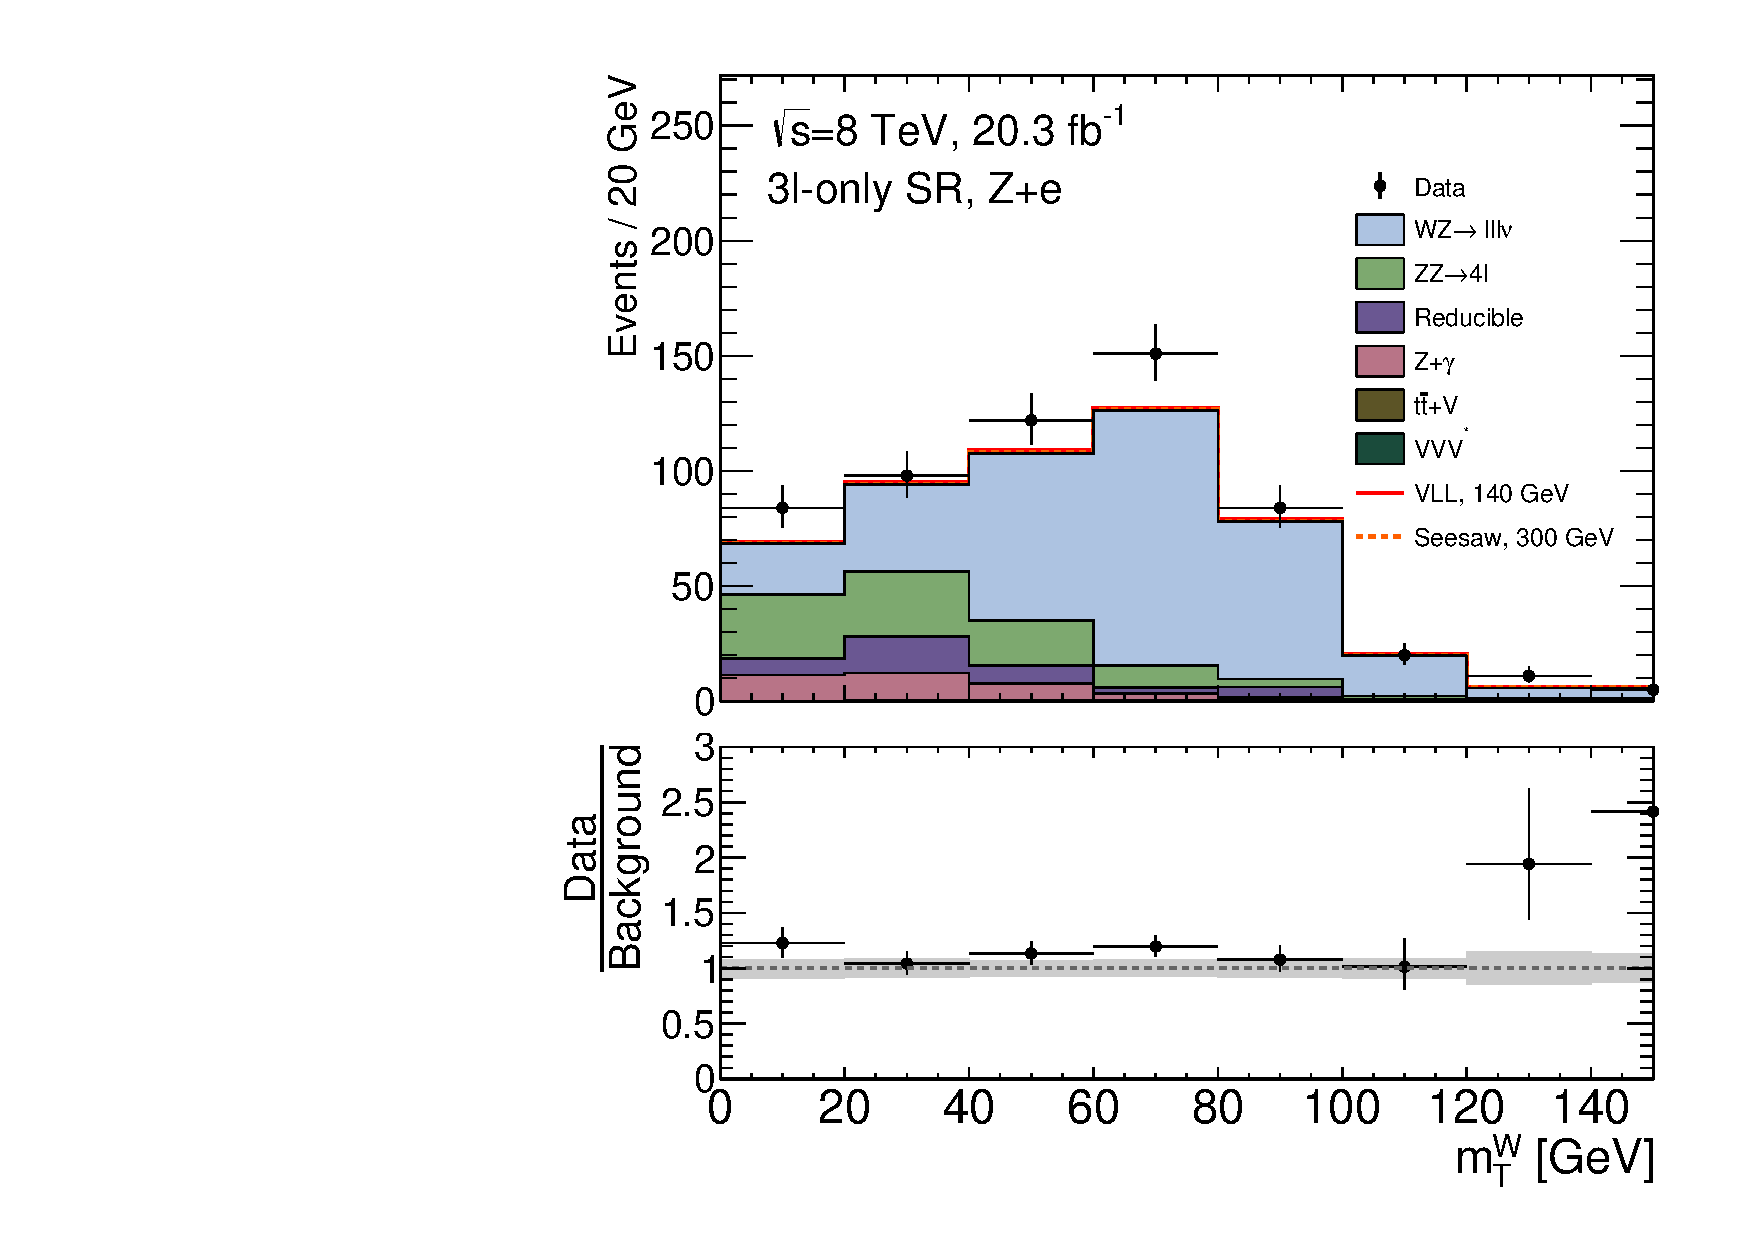
\includegraphics{figures/resonance/c_output_mTW_Ze_ElseNoM3L_300GeV}}
  }
  \subfloat[ $Z+\mu$, else category] {
    \resizebox{0.48\textwidth}{!}{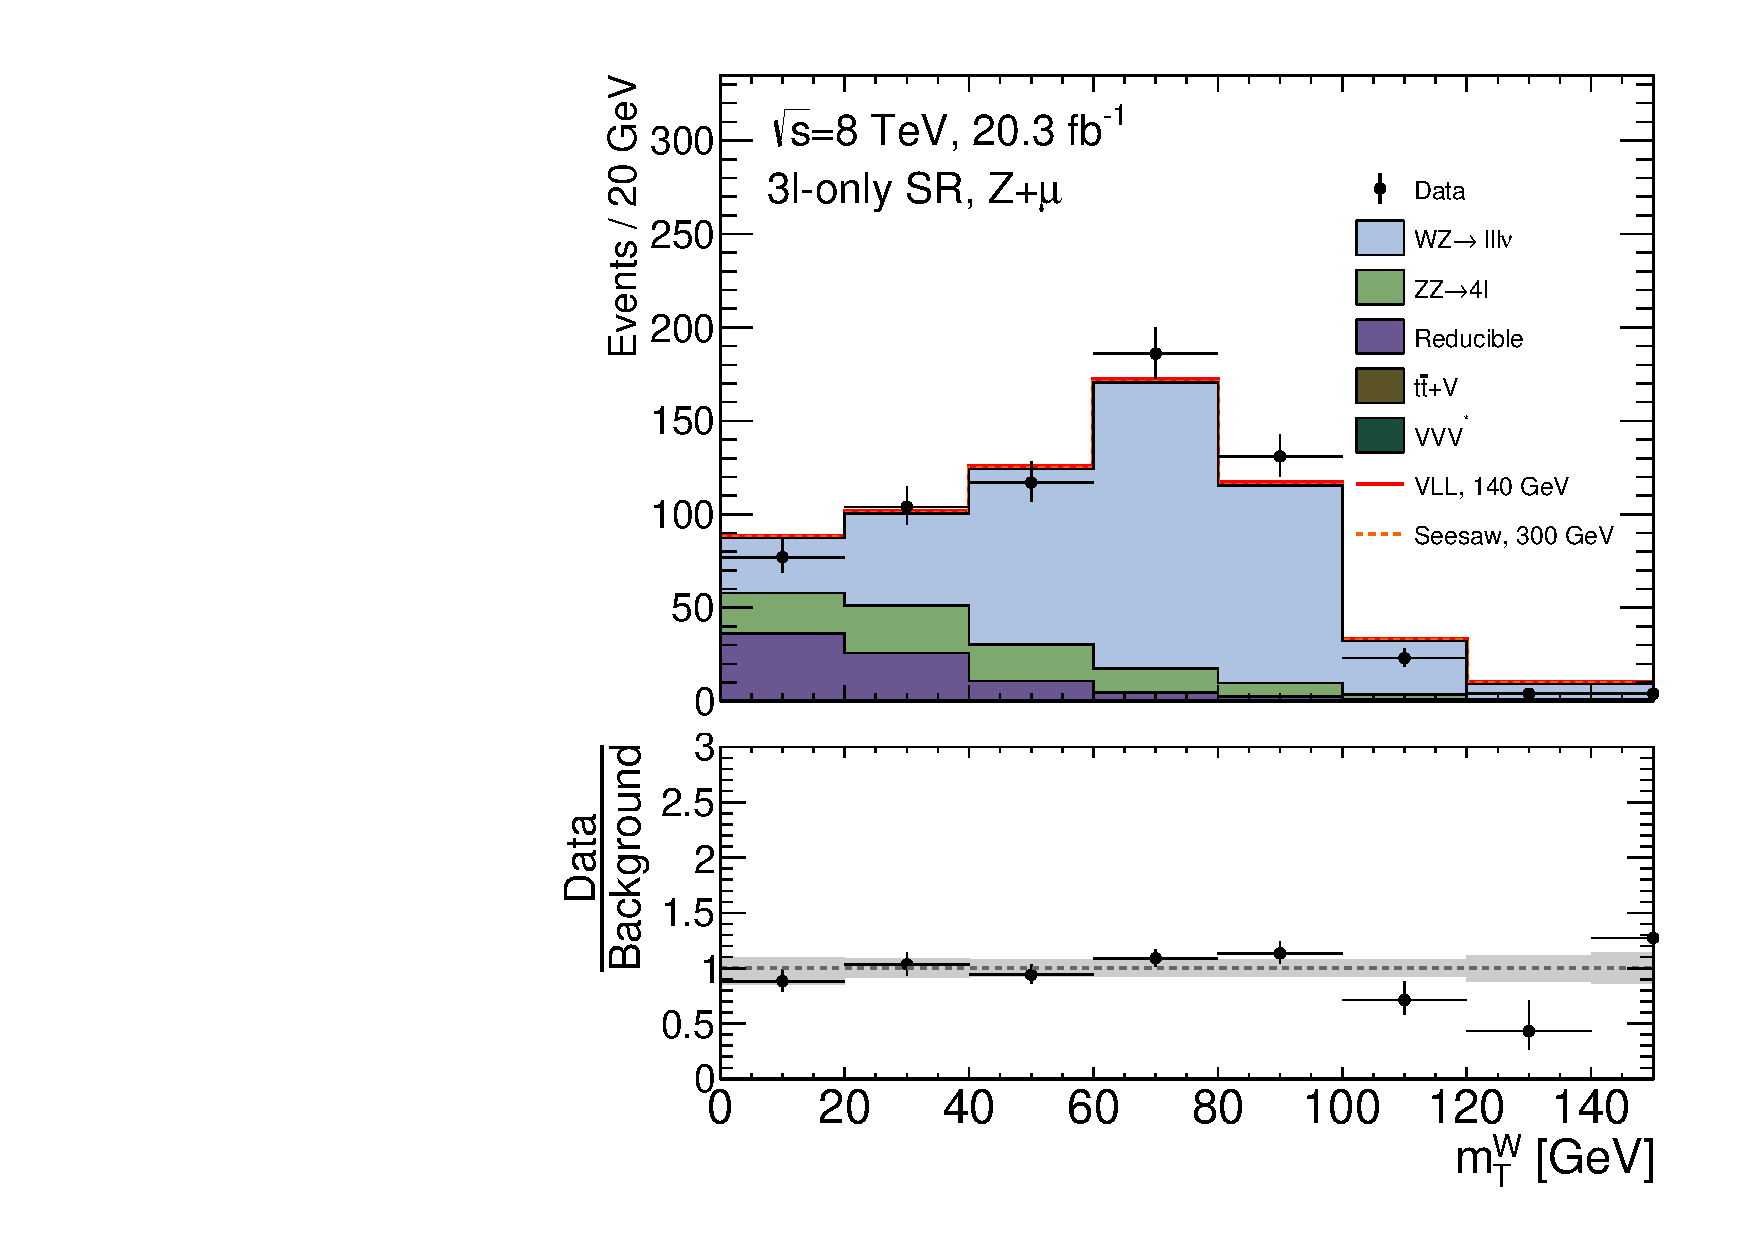
\includegraphics{figures/resonance/c_output_mTW_Zmu_ElseNoM3L_300GeV}}
  }
  \caption{Transverse mass of the missing energy and bachelor lepton ($\mtw$) for $Z+e$ and $Z+\mu$ candidates, for the $\threeljj$ and $\threelo$ signal regions.}
  \label{fig:SR-mTW-2}
\end{figure}

\clearpage

\begin{figure}[htb]
  \centering
  \subfloat[ $Z+e$, inclusive] {
    \resizebox{0.48\textwidth}{!}{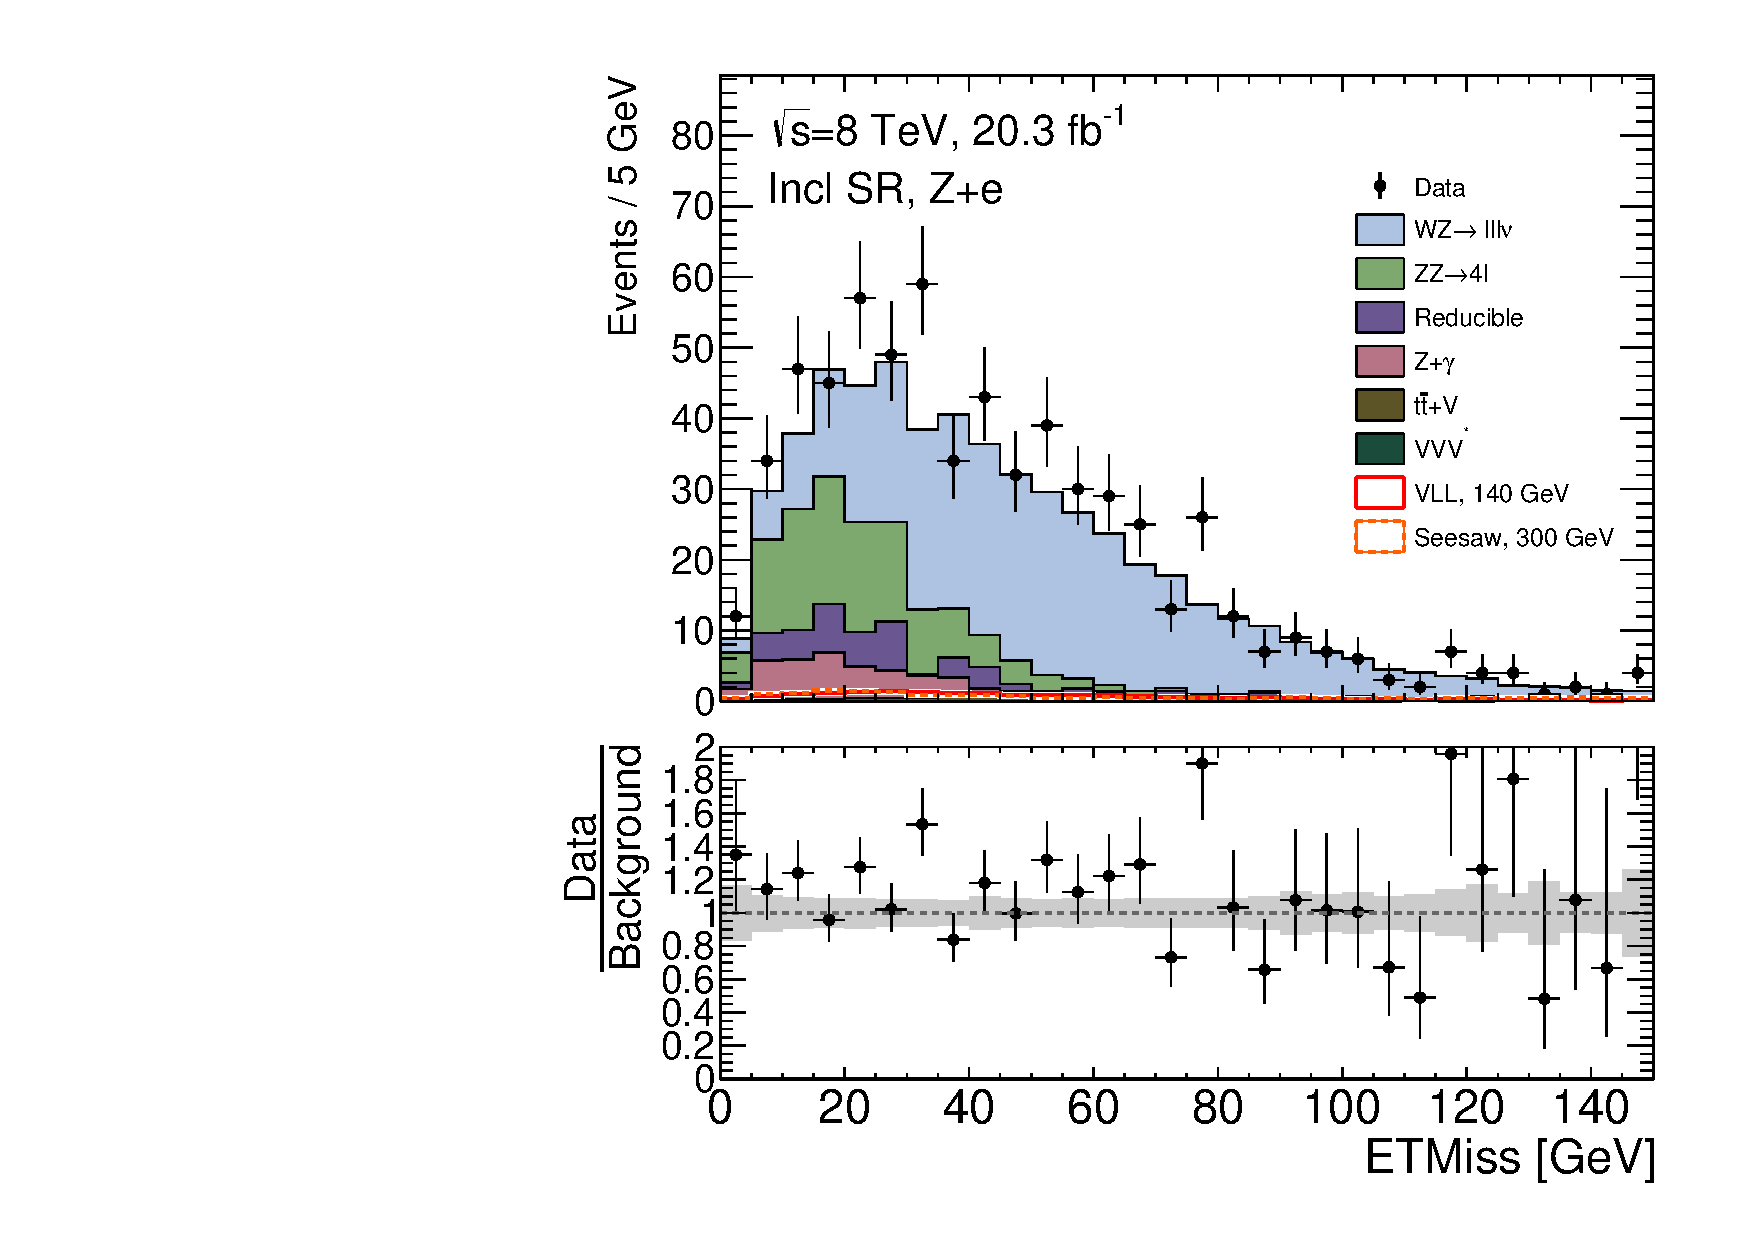
\includegraphics{figures/resonance/c_output_ETMiss_Ze_InclusiveNoM3L_300GeV}}
  }
  \subfloat[ $Z+\mu$, inclusive] {
    \resizebox{0.48\textwidth}{!}{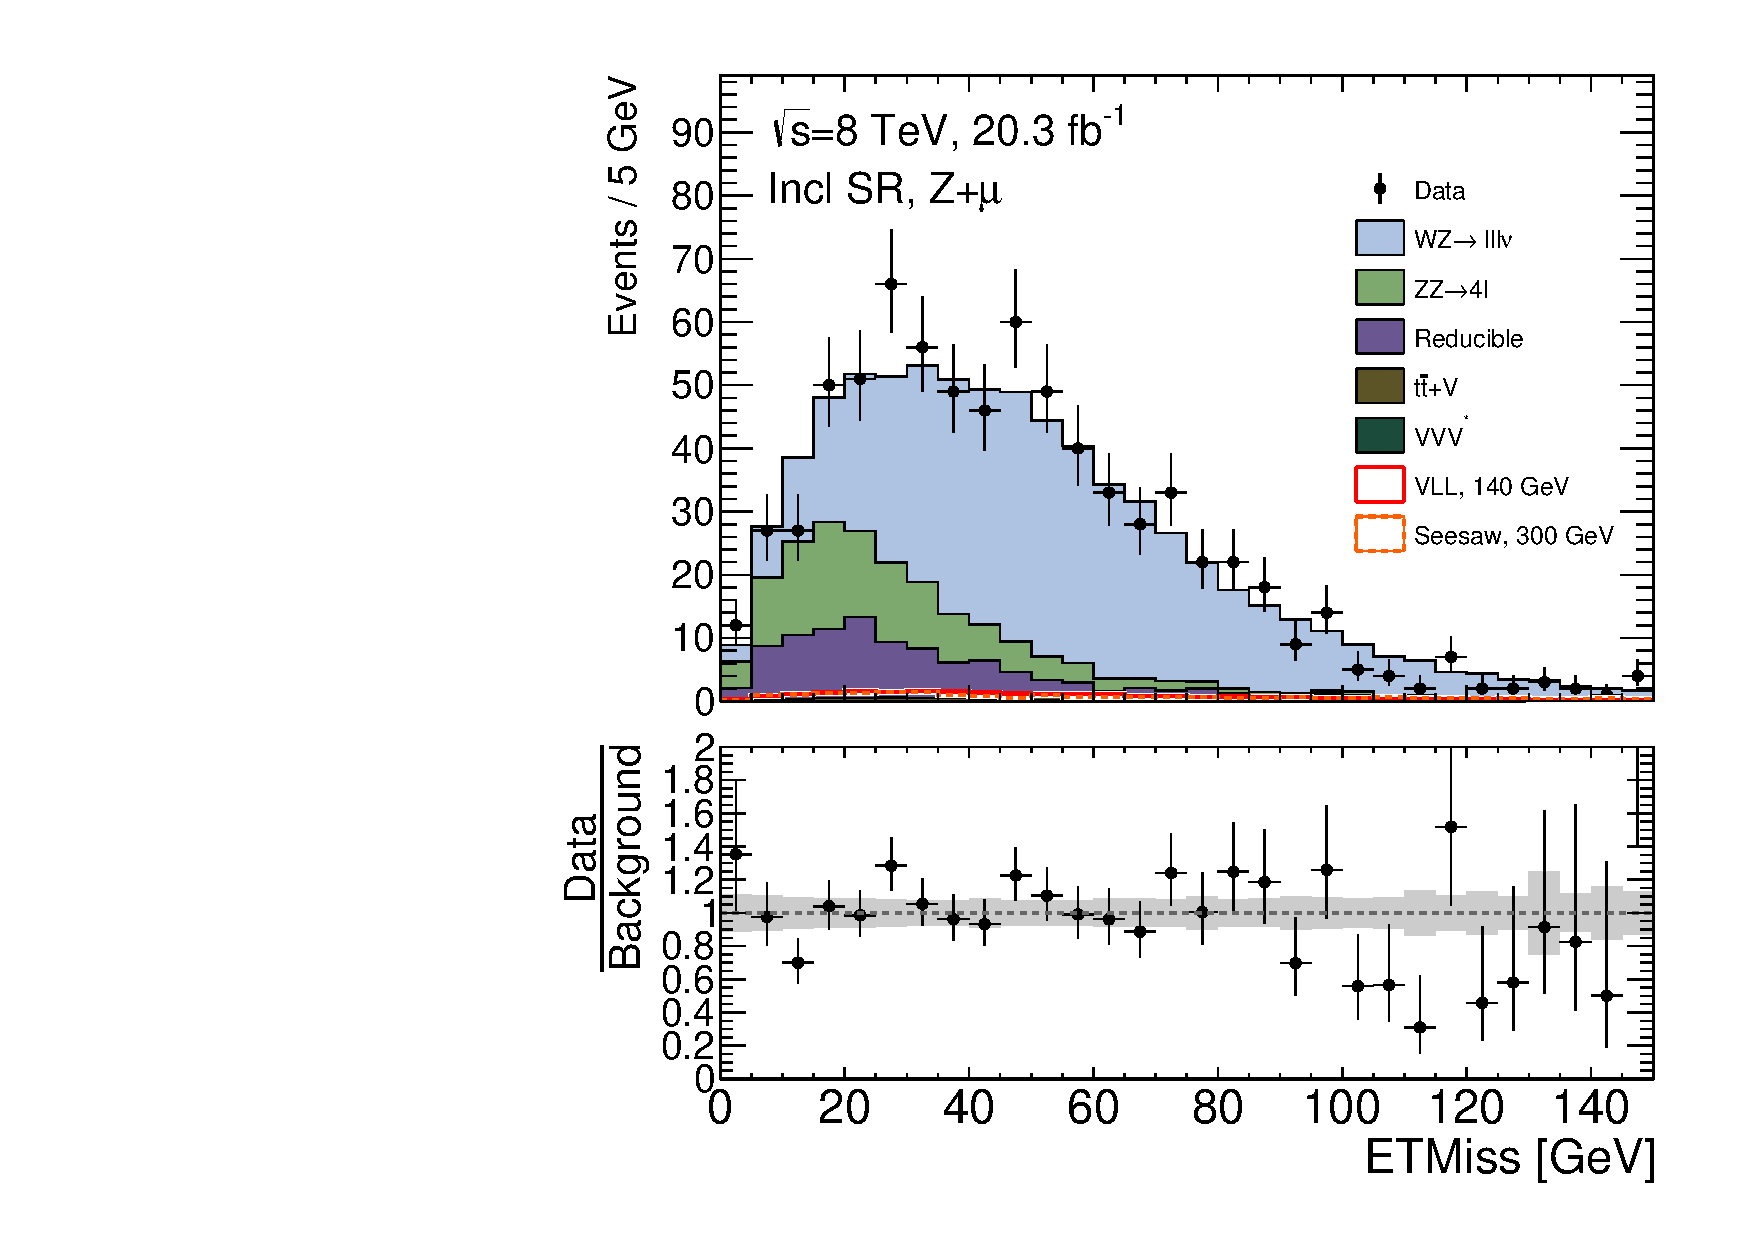
\includegraphics{figures/resonance/c_output_ETMiss_Zmu_InclusiveNoM3L_300GeV}}
  } \\
  \subfloat[ $Z+e$, $4L$ category] {
    \resizebox{0.48\textwidth}{!}{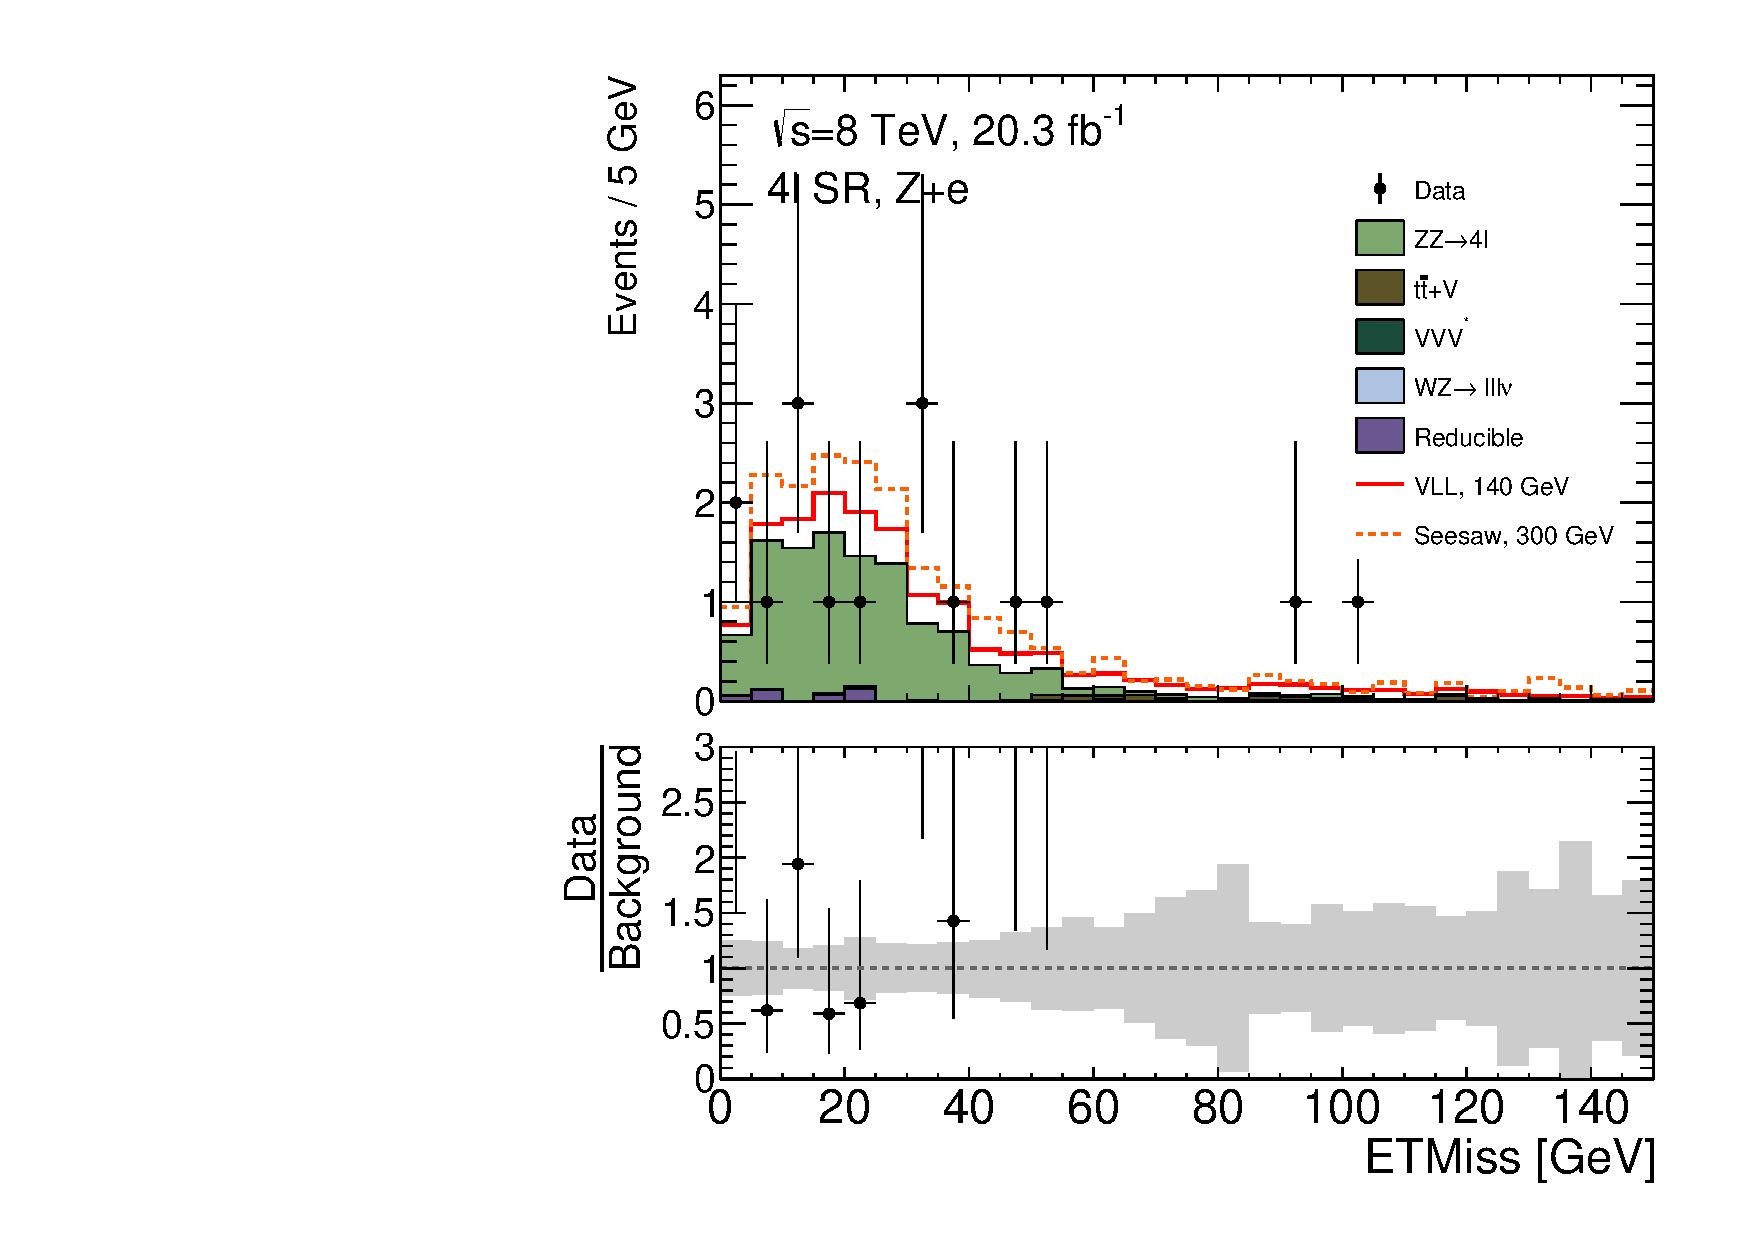
\includegraphics{figures/resonance/c_output_ETMiss_Ze_FourLNoM3L_300GeV}}
  }
  \subfloat[ $Z+\mu$, $4L$ category] {
    \resizebox{0.48\textwidth}{!}{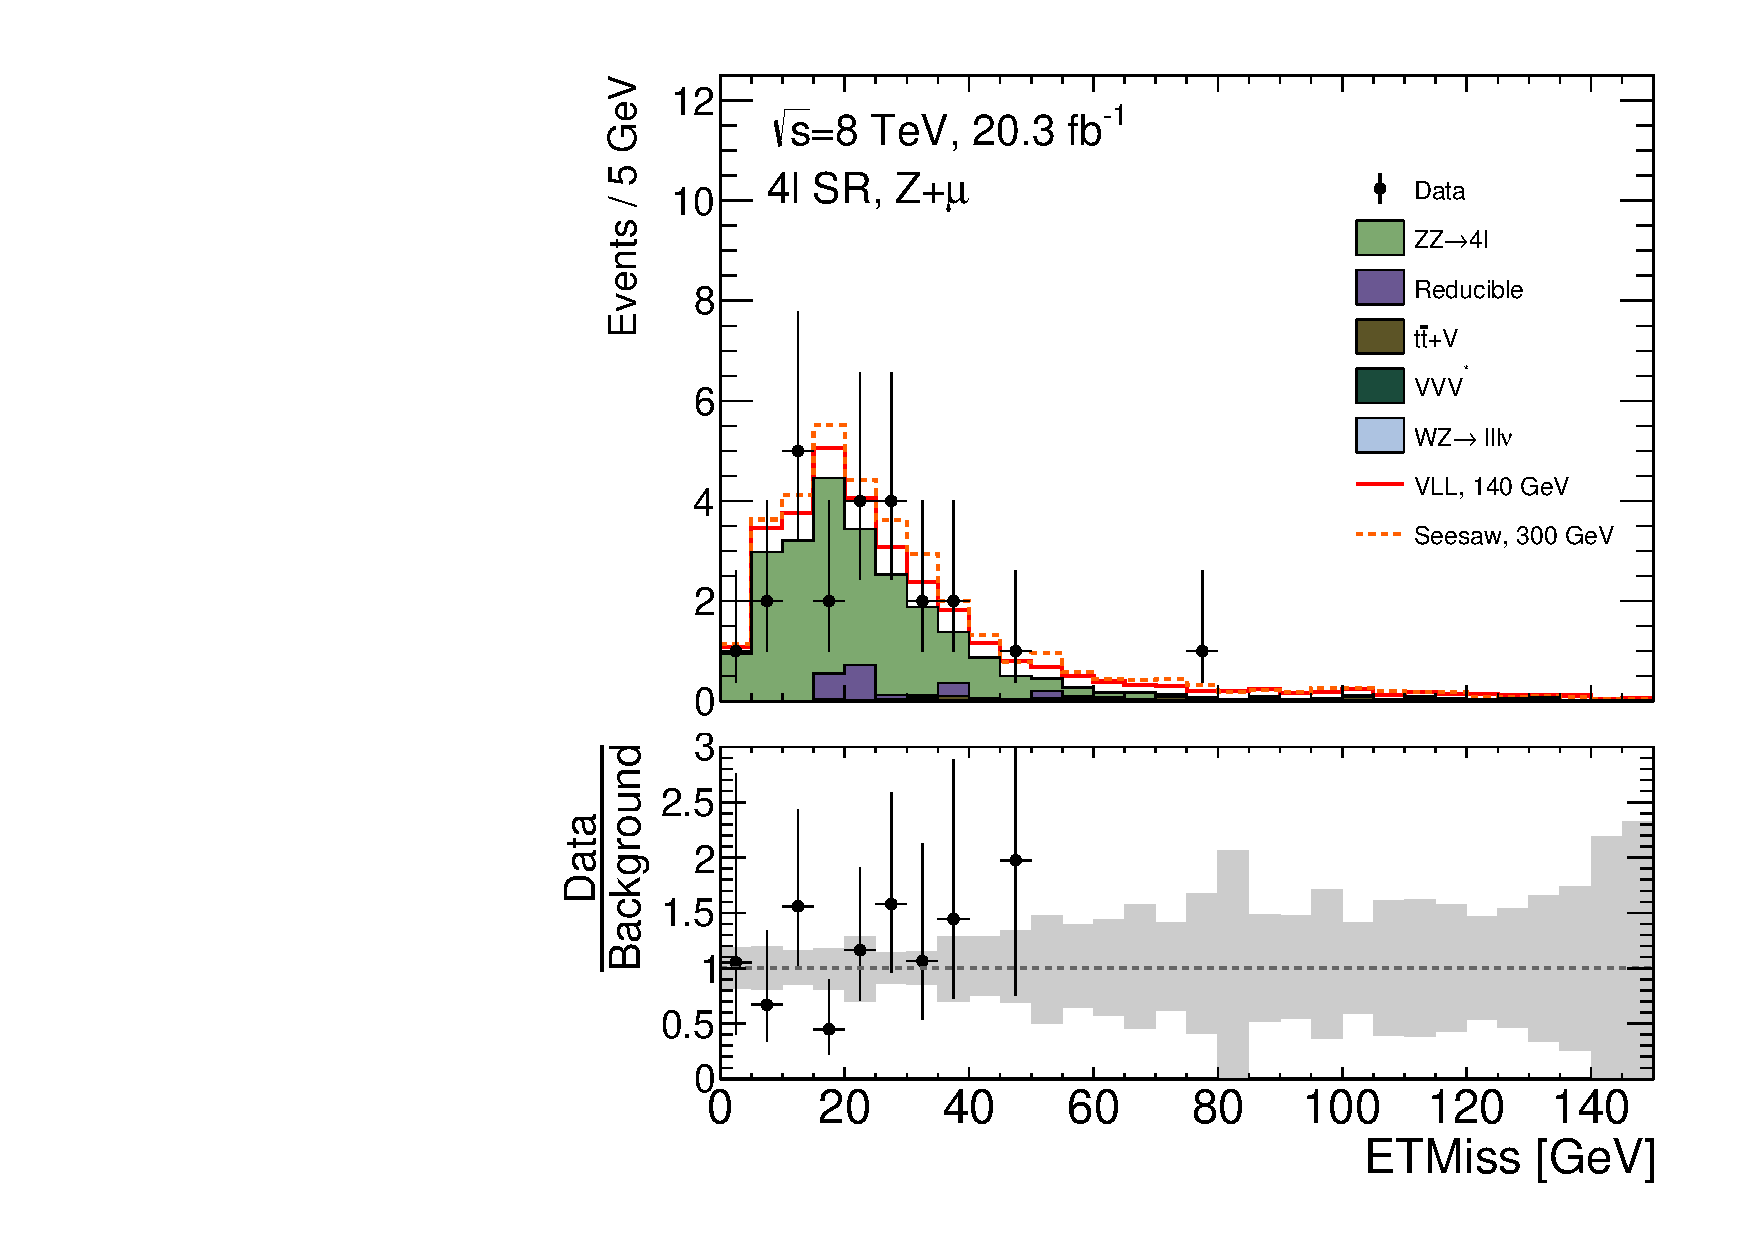
\includegraphics{figures/resonance/c_output_ETMiss_Zmu_FourLNoM3L_300GeV}}
  } \\
  \caption{Missing energy ($\Etmiss$) for $Z+e$ and $Z+\mu$ candidates, for the inclusive and $\fourl$ signal regions.}
  \label{fig:SR-ETMiss-1}
\end{figure}

\clearpage

\begin{figure}[htb]
  \centering
  \subfloat[ $Z+e$, dijet category] {
    \resizebox{0.48\textwidth}{!}{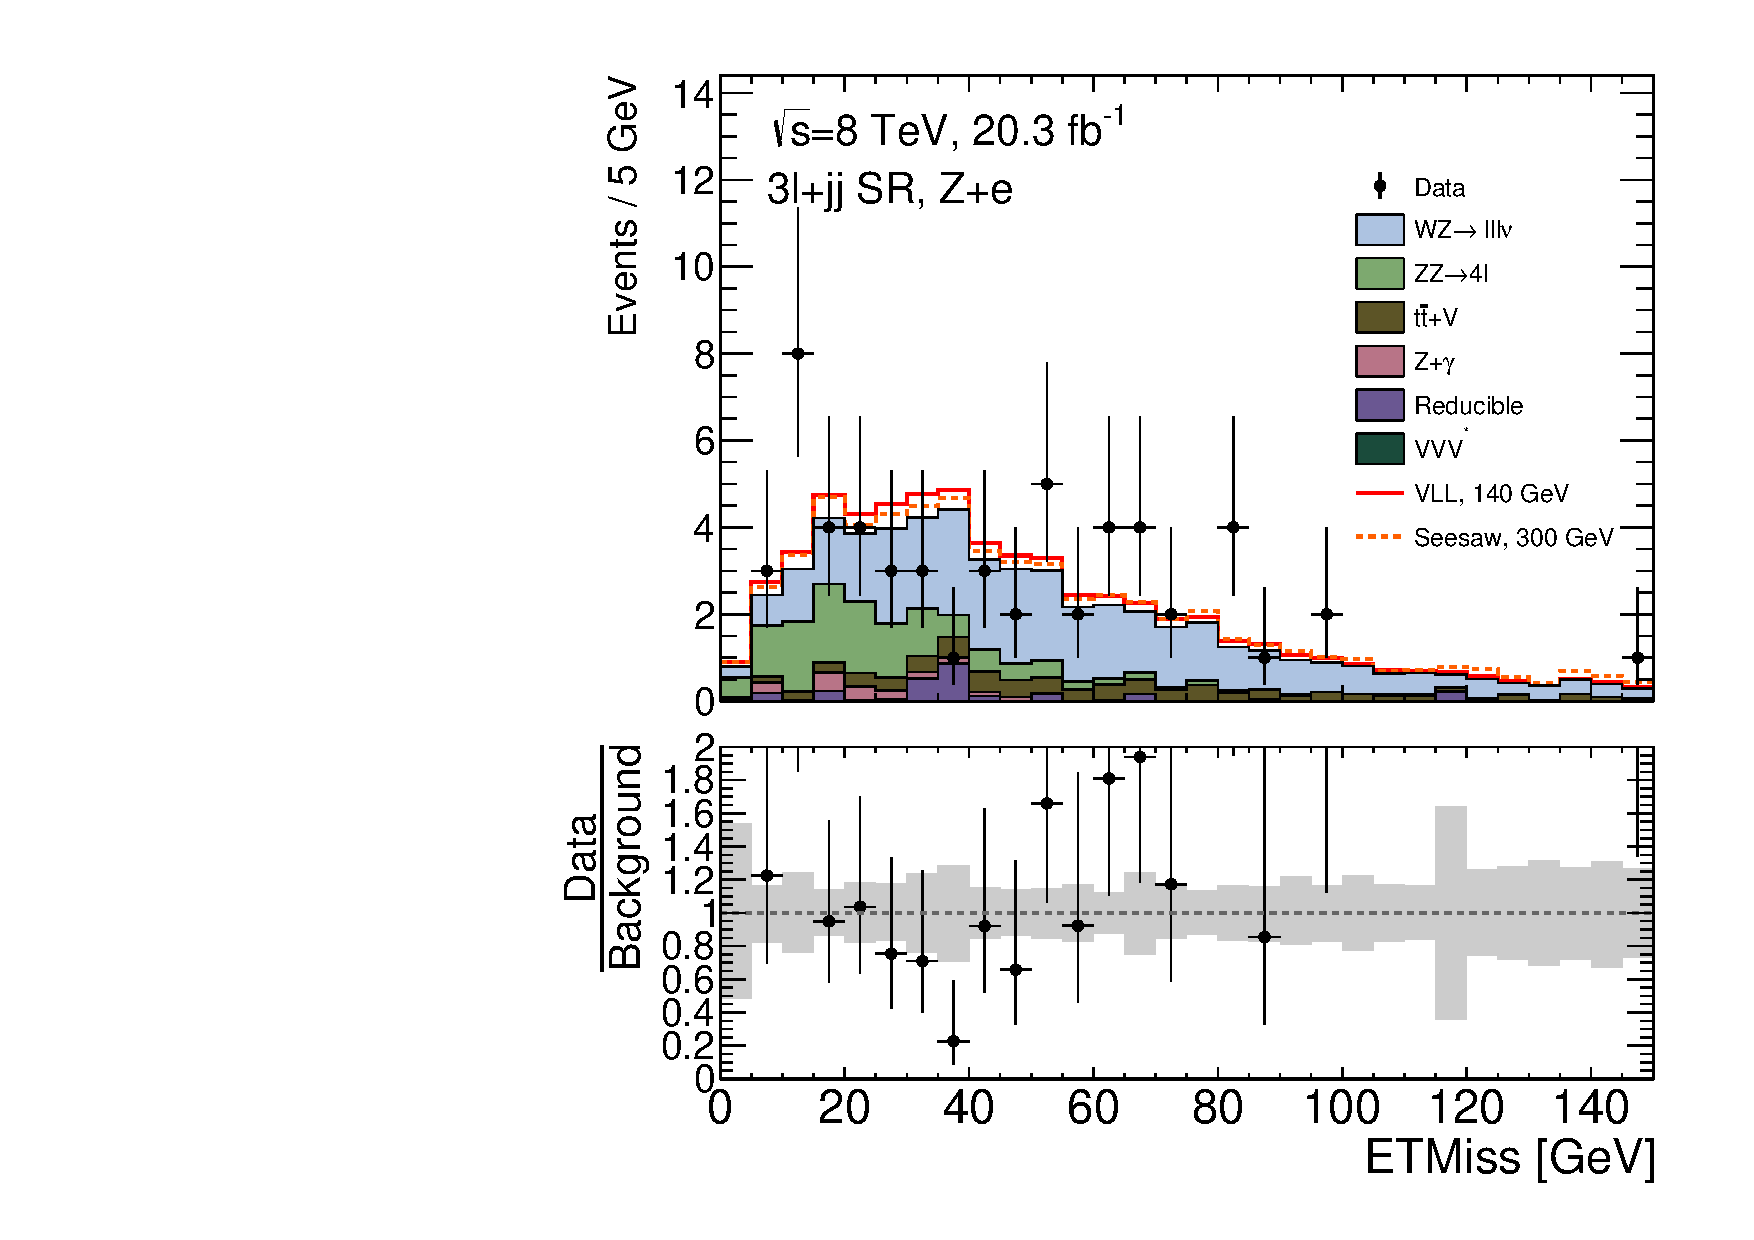
\includegraphics{figures/resonance/c_output_ETMiss_Ze_ThreeLDijetNoM3L_300GeV}}
  }
  \subfloat[ $Z+\mu$, dijet category] {
    \resizebox{0.48\textwidth}{!}{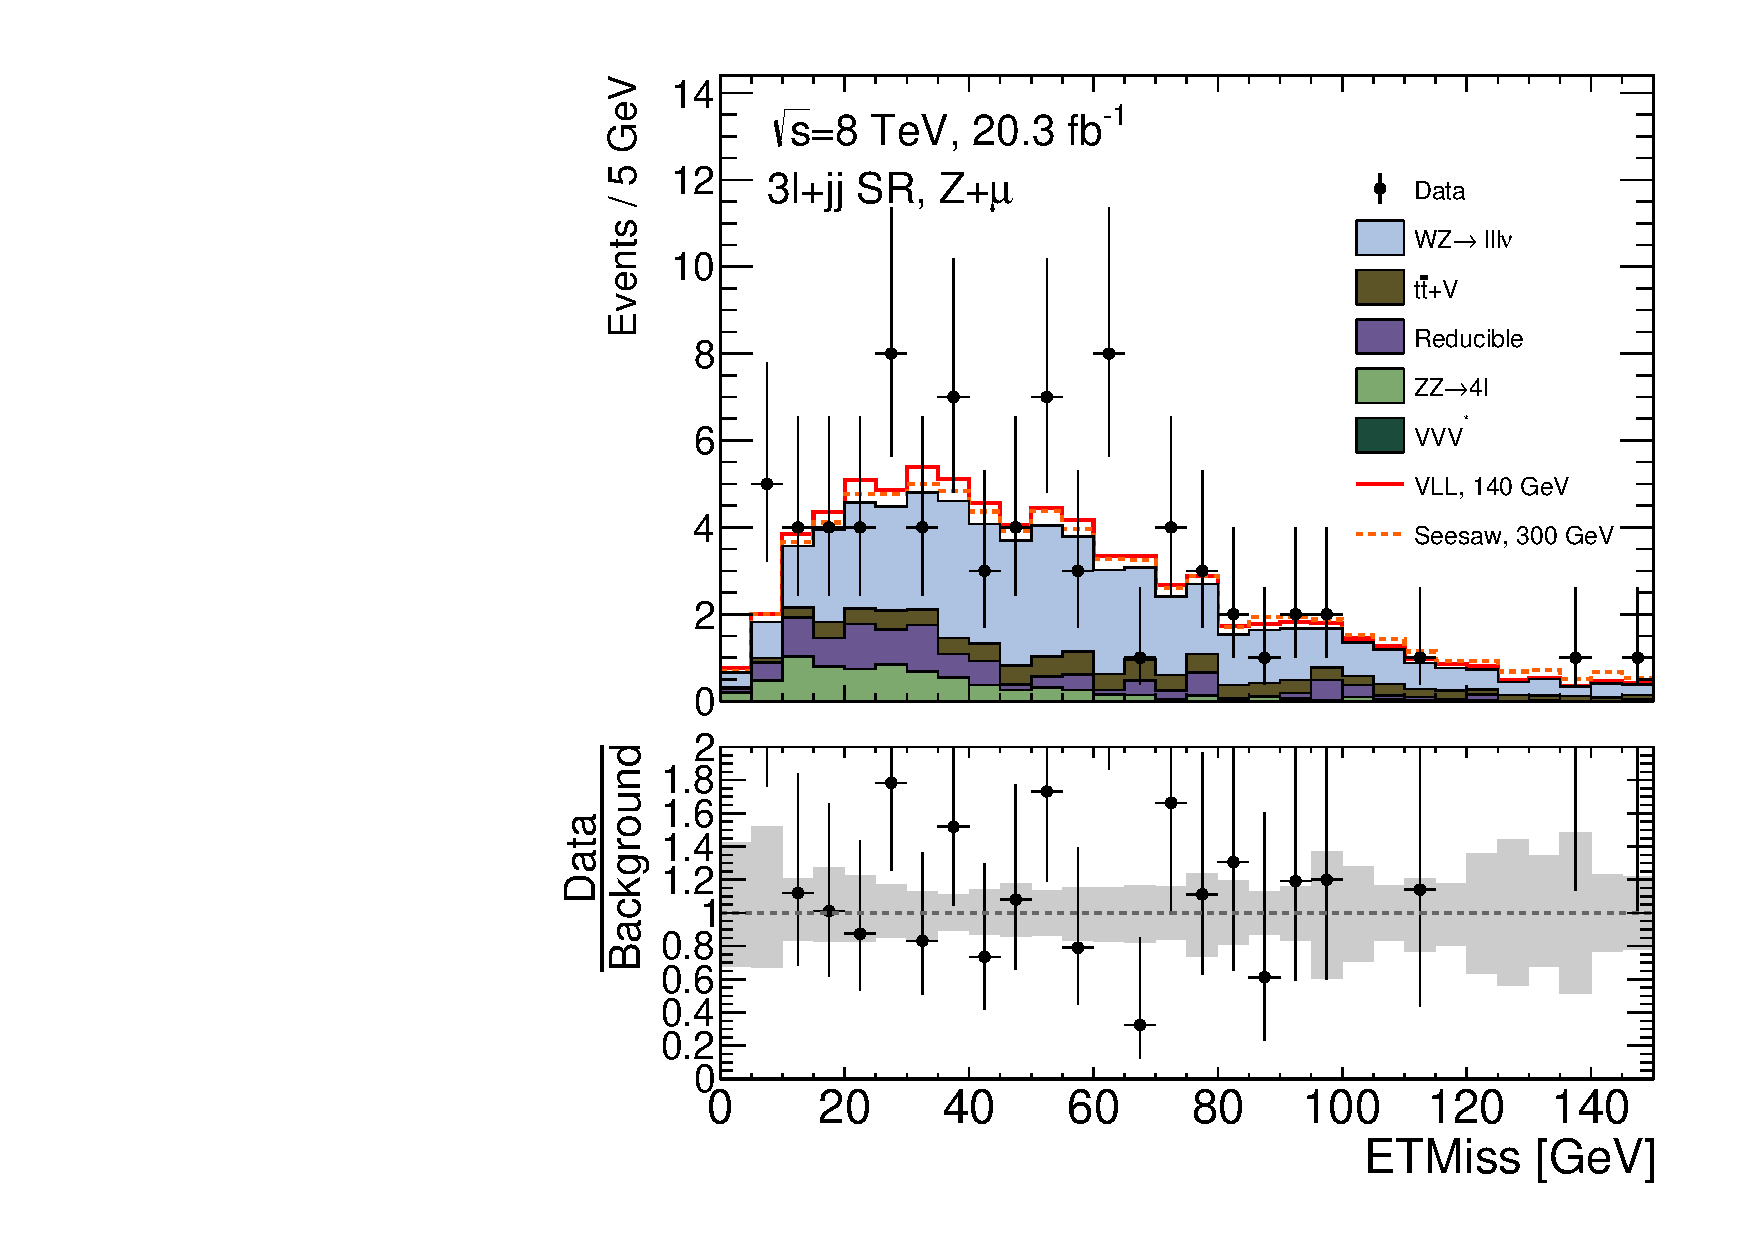
\includegraphics{figures/resonance/c_output_ETMiss_Zmu_ThreeLDijetNoM3L_300GeV}}
  } \\
  \subfloat[ $Z+e$, else category] {
    \resizebox{0.48\textwidth}{!}{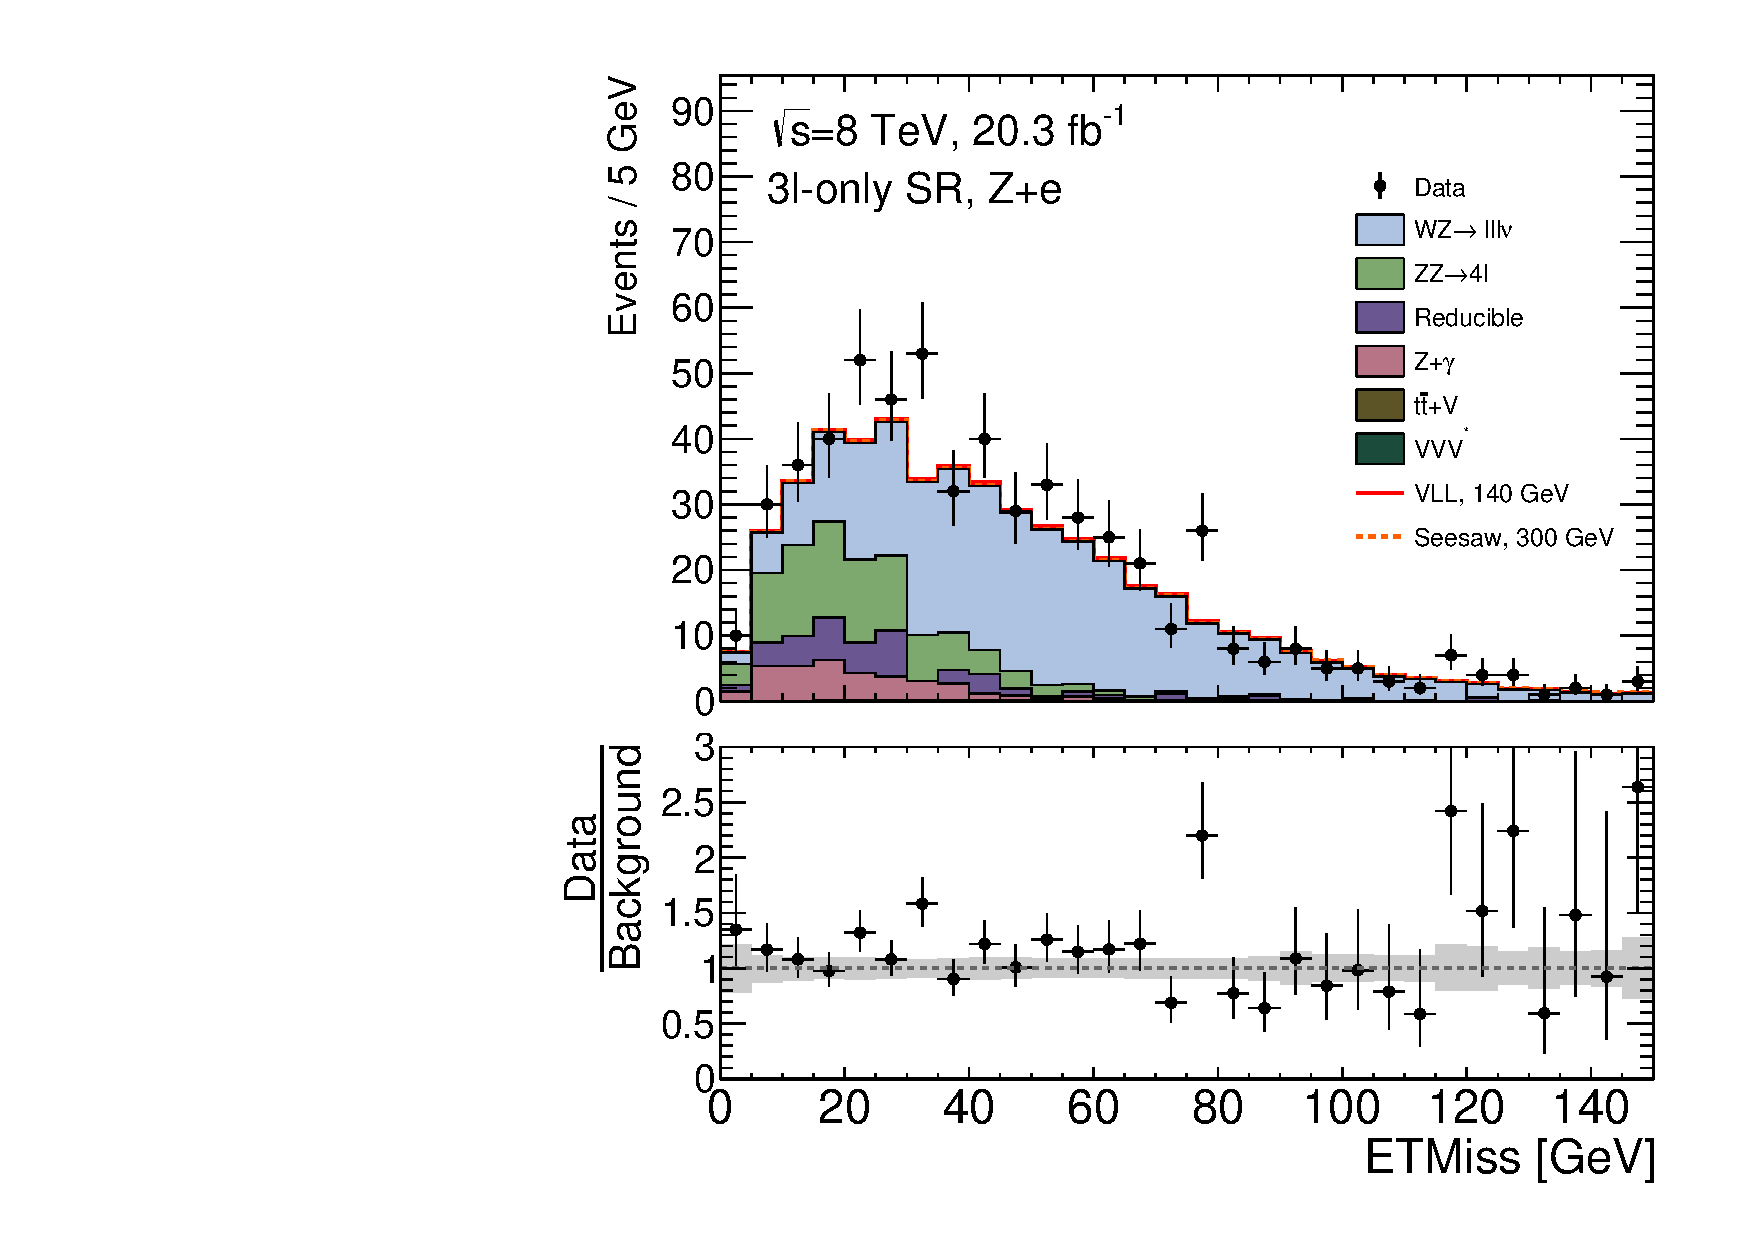
\includegraphics{figures/resonance/c_output_ETMiss_Ze_ElseNoM3L_300GeV}}
  }
  \subfloat[ $Z+\mu$, else category] {
    \resizebox{0.48\textwidth}{!}{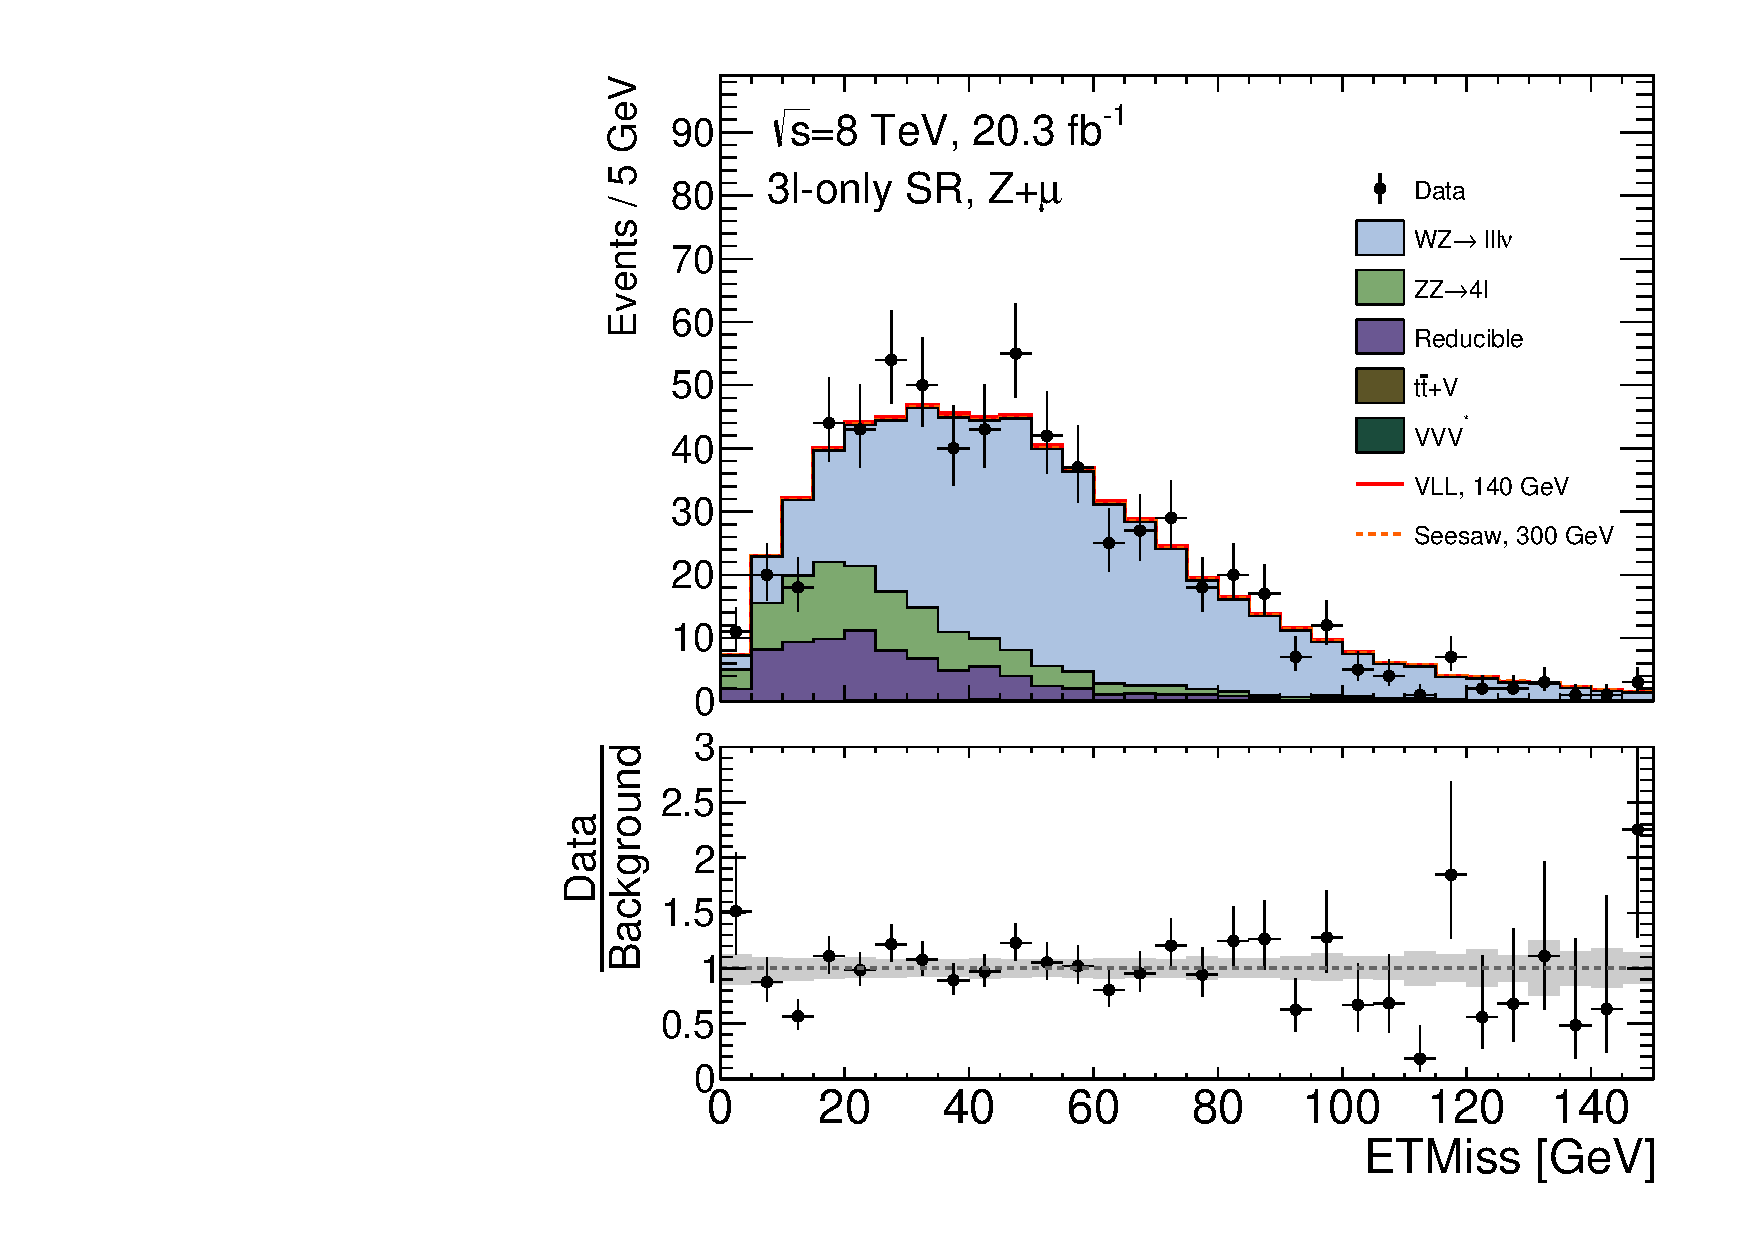
\includegraphics{figures/resonance/c_output_ETMiss_Zmu_ElseNoM3L_300GeV}}
  }
  \caption{Missing energy ($\Etmiss$) for $Z+e$ and $Z+\mu$ candidates, for the $\threeljj$ and $\threelo$ signal regions.}
  \label{fig:SR-ETMiss-2}
\end{figure}

\clearpage
